\chapter{Results} \label{appendix:results}

\section{Cluster utility} \label{appendix:results-cluster-utility}
\subsection{2-Dimensional data}
\mycomment{\begin{figure}[H]
        \caption{External validation for all mechanisms the 2-dimensional data seeds-dataset}
        \centering
        \begin{minipage}[c]{0.49\textwidth}
            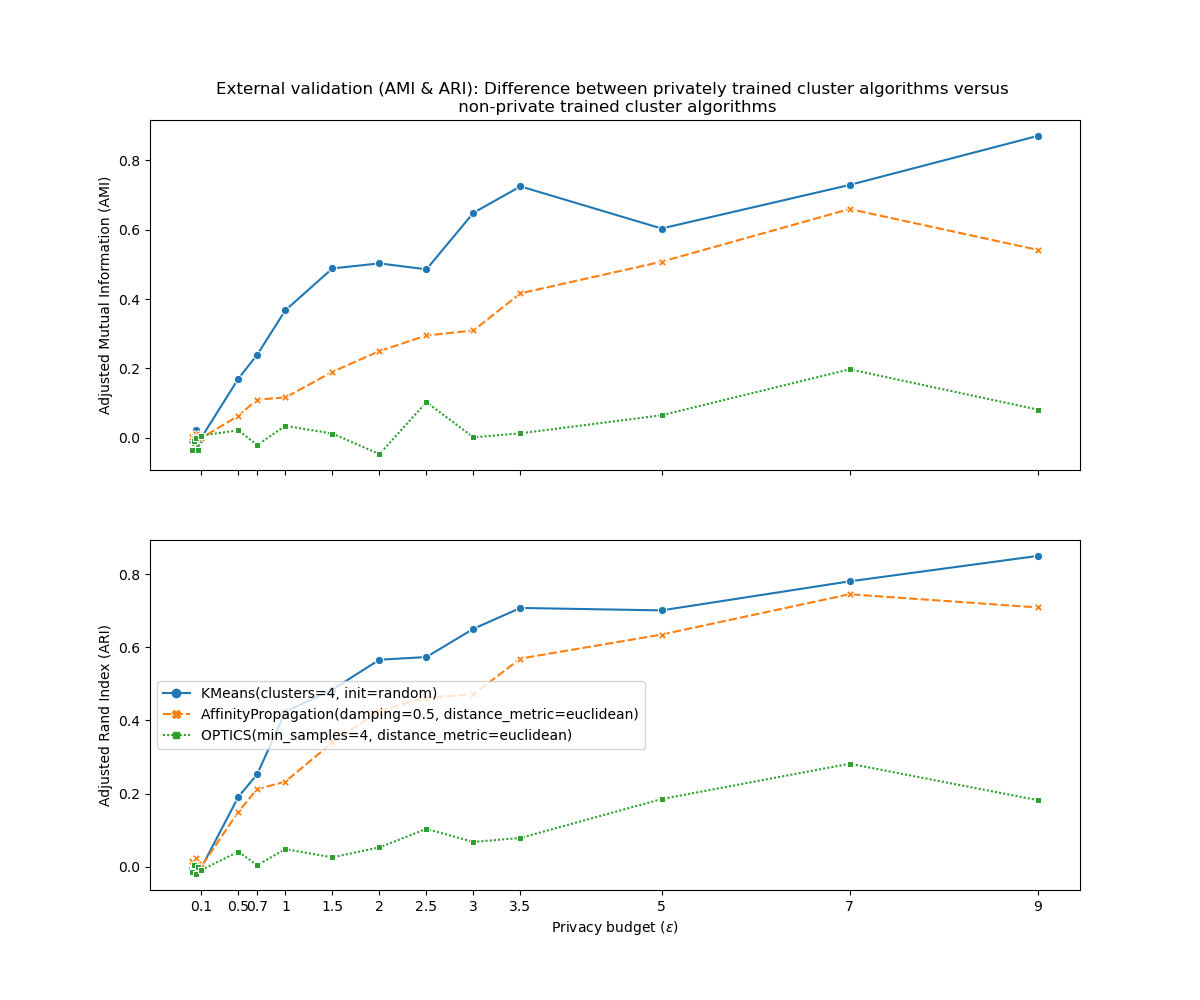
\includegraphics[width=1\textwidth]{Results/2d-laplace/seeds-dataset/ami-and-ari.png}
            \caption{External validation (ARI/ AMI) for the 2-dimensional data seeds-dataset for laplace.}
            \label{fig:appendix-external-validation-seeds-dataset_comparison_2d-laplace}
        \end{minipage}
        \begin{minipage}[c]{0.49\textwidth}
            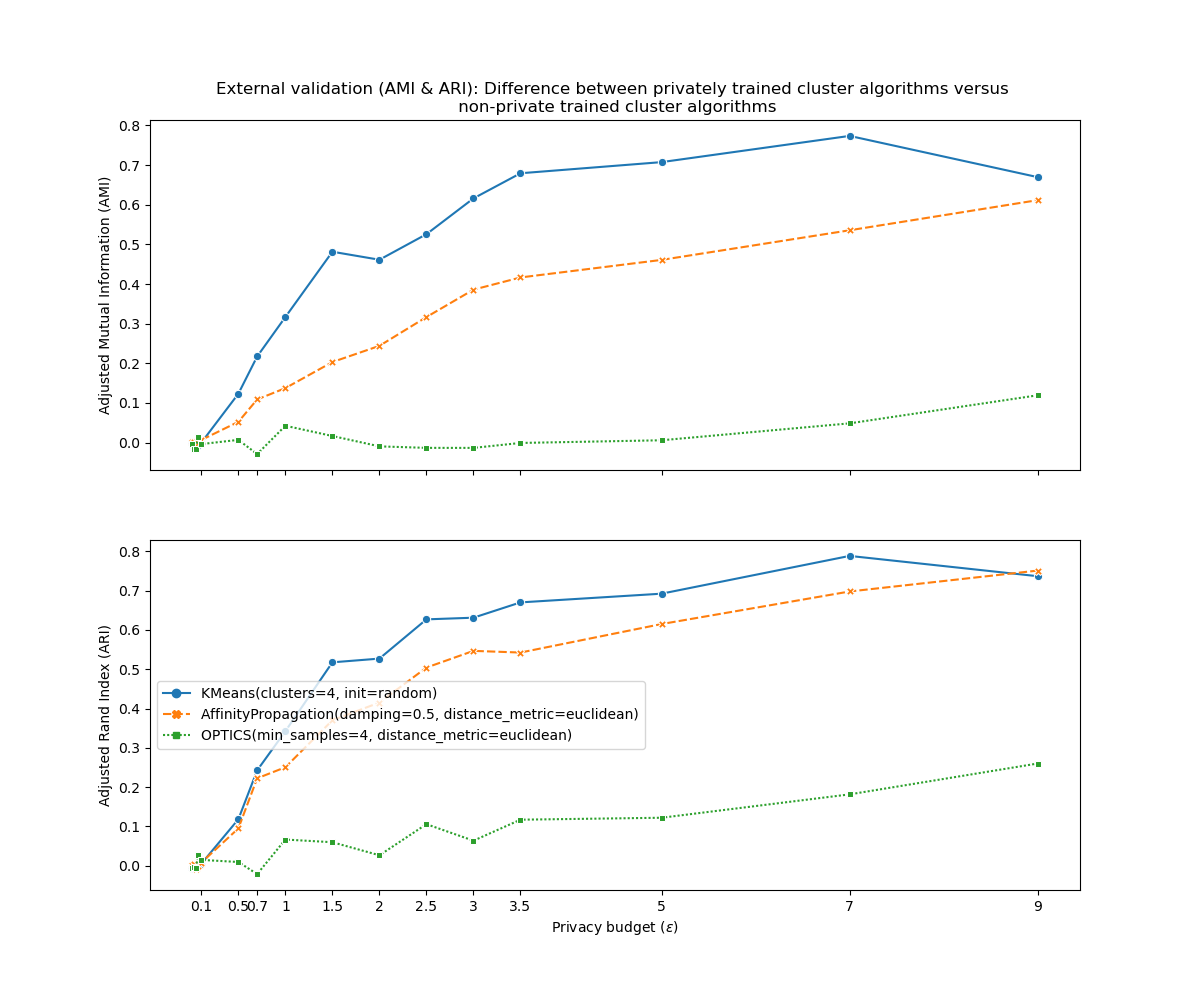
\includegraphics[width=1\textwidth]{Results/2d-laplace-truncated/seeds-dataset/ami-and-ari.png}
            \caption{External validation (ARI/ AMI) for the 2-dimensional data seeds-dataset for laplace with truncation.}
            \label{fig:appendix-external-validation-seeds-dataset_comparison_2d-laplace-truncated}
        \end{minipage}
        \begin{minipage}[c]{0.49\textwidth}
            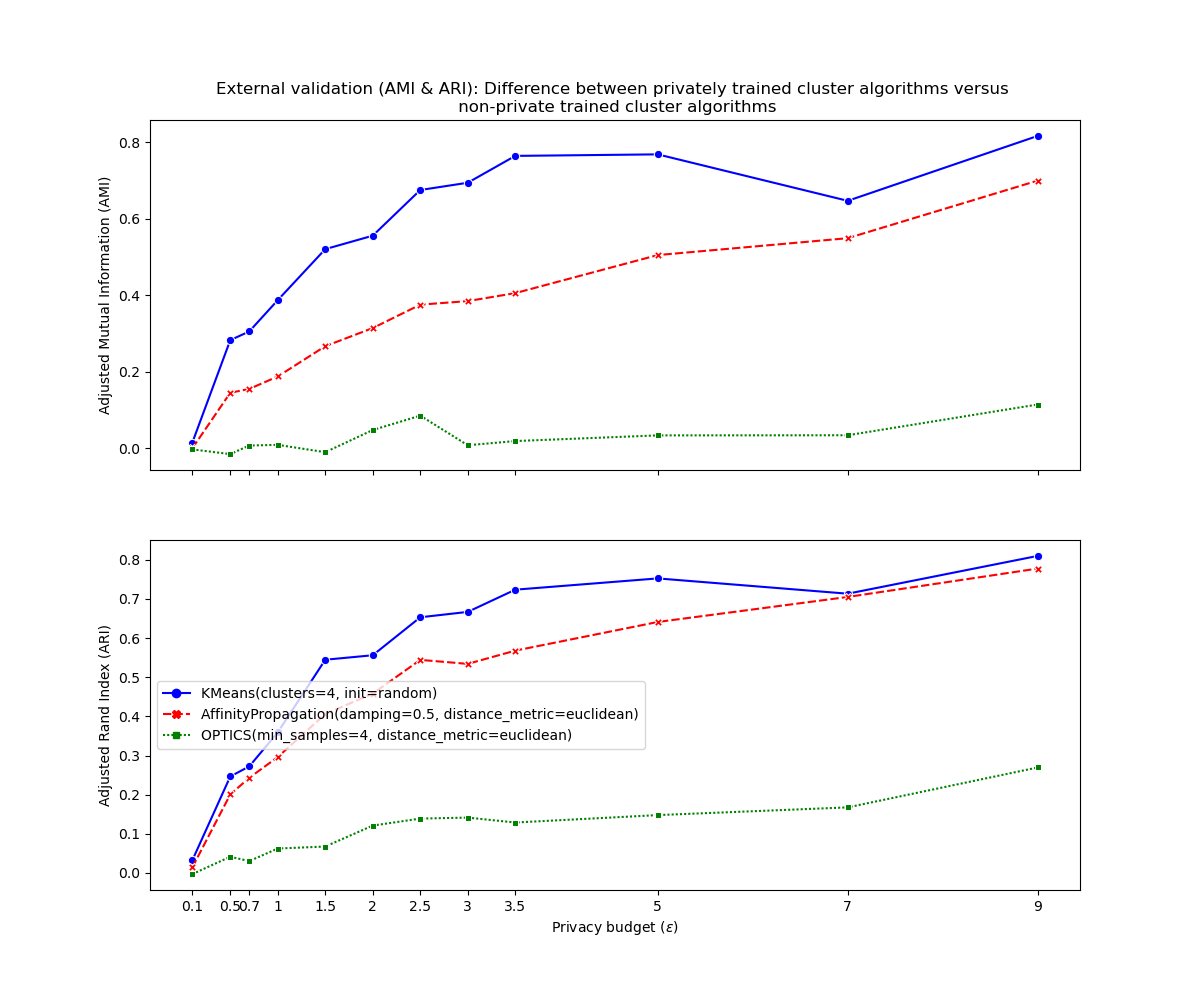
\includegraphics[width=1\textwidth]{Results/2d-laplace-optimal-truncated/seeds-dataset/ami-and-ari.png}
            \caption{External validation (ARI/ AMI) for the 2-dimensional data seeds-dataset for laplace with optimal truncation}
            \label{fig:appendix-external-validation-seeds-dataset_comparison_2d-laplace-optimal-truncated}
        \end{minipage}
        \begin{minipage}[c]{0.49\textwidth}
            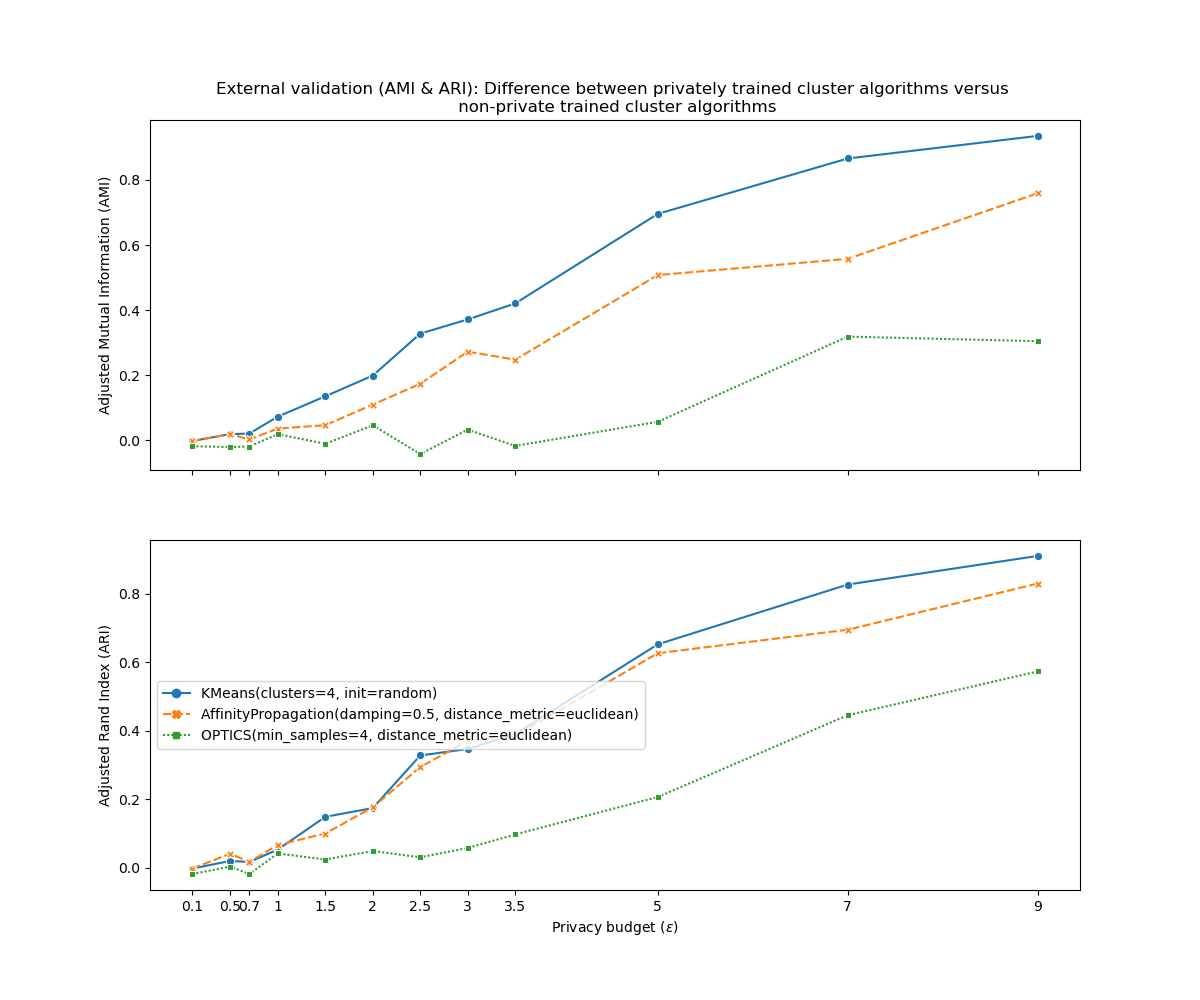
\includegraphics[width=1\textwidth]{Results/2d-piecewise/seeds-dataset/ami-and-ari.png}
            \caption{External validation (ARI/ AMI) for the 2-dimensional data seeds-dataset for piecewise mechanism}
            \label{fig:appendix-external-validation-seeds-dataset_comparison_2d-piecewise}
        \end{minipage}
    \end{figure}}

\begin{figure}[H]
    \caption{Internal validation for all mechanisms the 2-dimensional data heart-dataset}
    \centering
    \begin{minipage}[c]{0.49\textwidth}
        %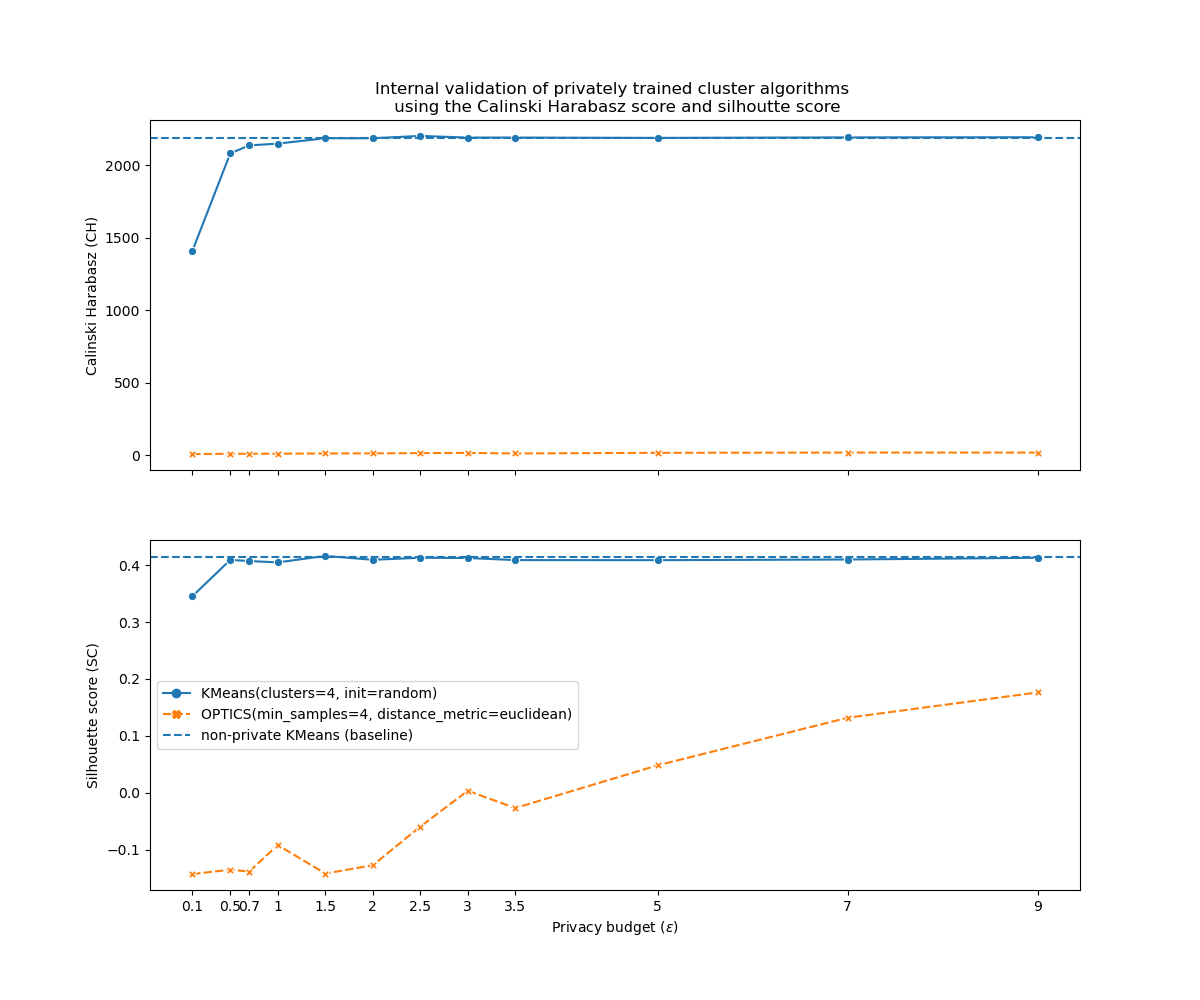
\includegraphics[width=1\textwidth]{Results/2d-laplace/heart-dataset/ch-and-sc.png}
        \caption{Internal validation (CH/ SC) for the 2-dimensional data heart-dataset for laplace.}
        \label{fig:appendix-internal-validation-heart-dataset_comparison_2d-laplace}
    \end{minipage}
    \begin{minipage}[c]{0.49\textwidth}
        %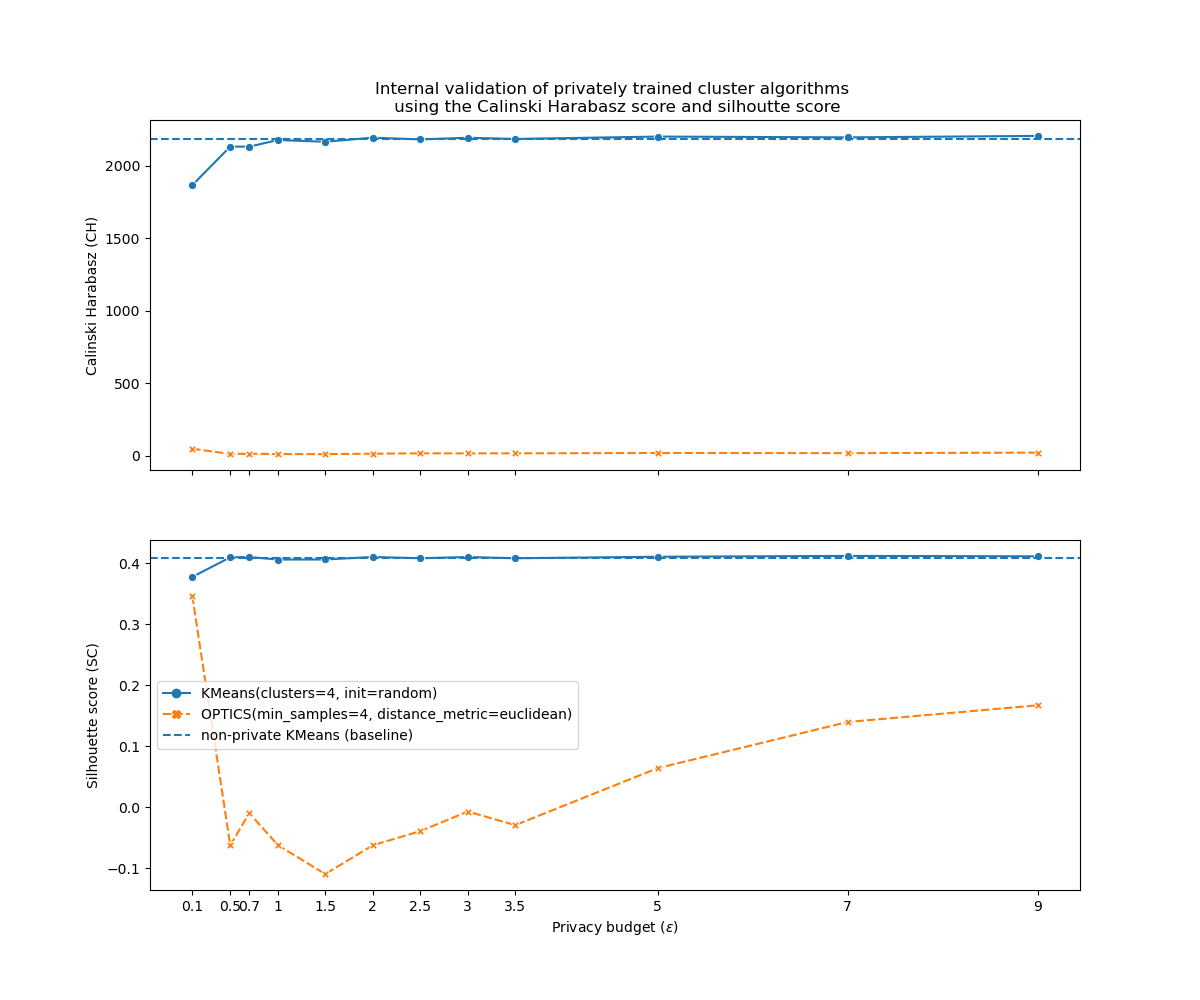
\includegraphics[width=1\textwidth]{Results/2d-laplace-truncated/heart-dataset/ch-and-sc.png}
        \caption{Internal validation (CH/ SC) for the 2-dimensional data heart-dataset for laplace with truncation.}
        \label{fig:appendix-internal-validation-heart-dataset_comparison_2d-laplace-truncated}
    \end{minipage}
    \begin{minipage}[c]{0.49\textwidth}
        %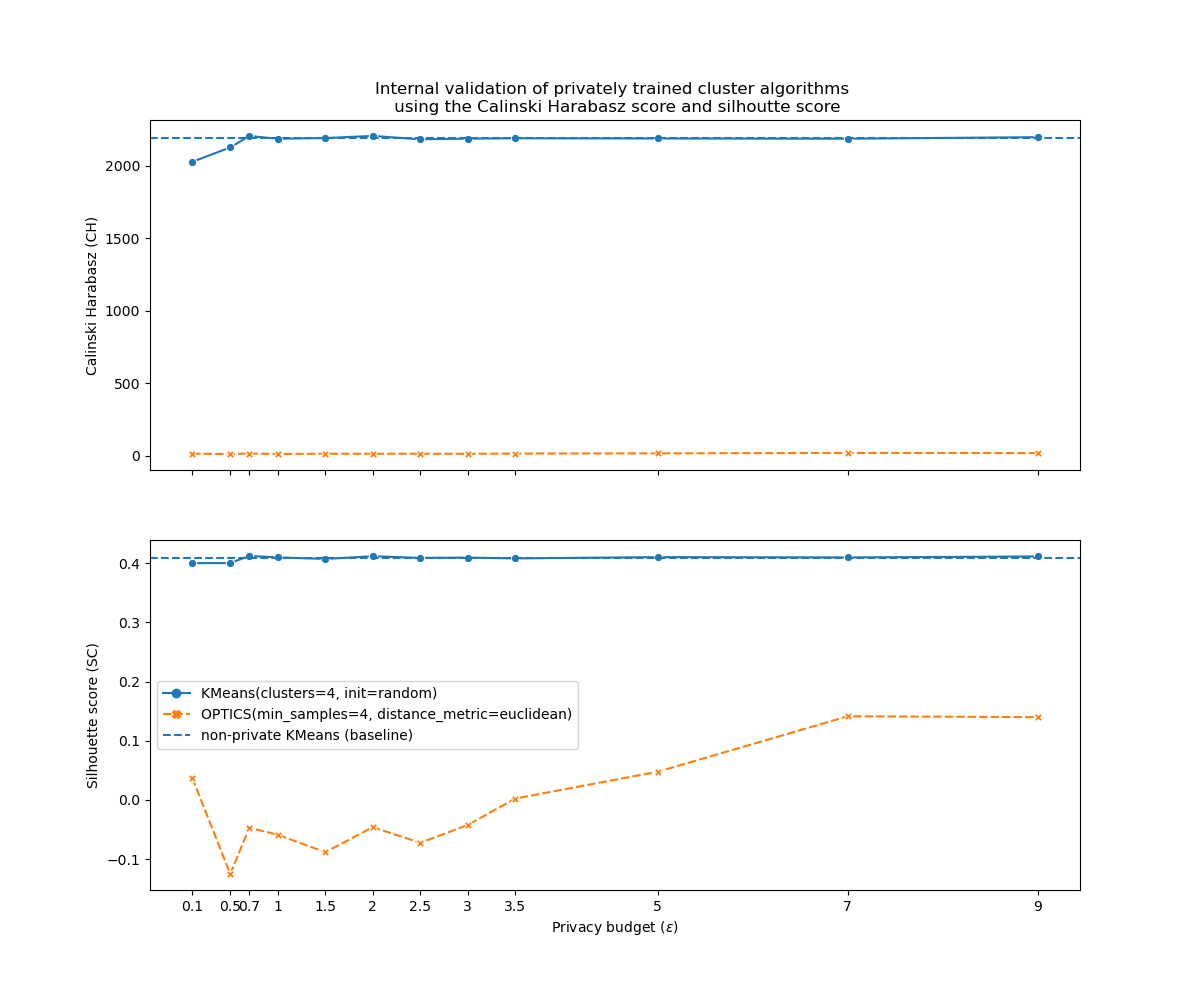
\includegraphics[width=1\textwidth]{Results/2d-laplace-optimal-truncated/heart-dataset/ch-and-sc.png}
        \caption{Internal validation (CH/ SC) for the 2-dimensional data heart-dataset for laplace with optimal truncation}
        \label{fig:appendix-internal-validation-heart-dataset_comparison_2d-laplace-optimal-truncated}
    \end{minipage}
    \begin{minipage}[c]{0.49\textwidth}
        %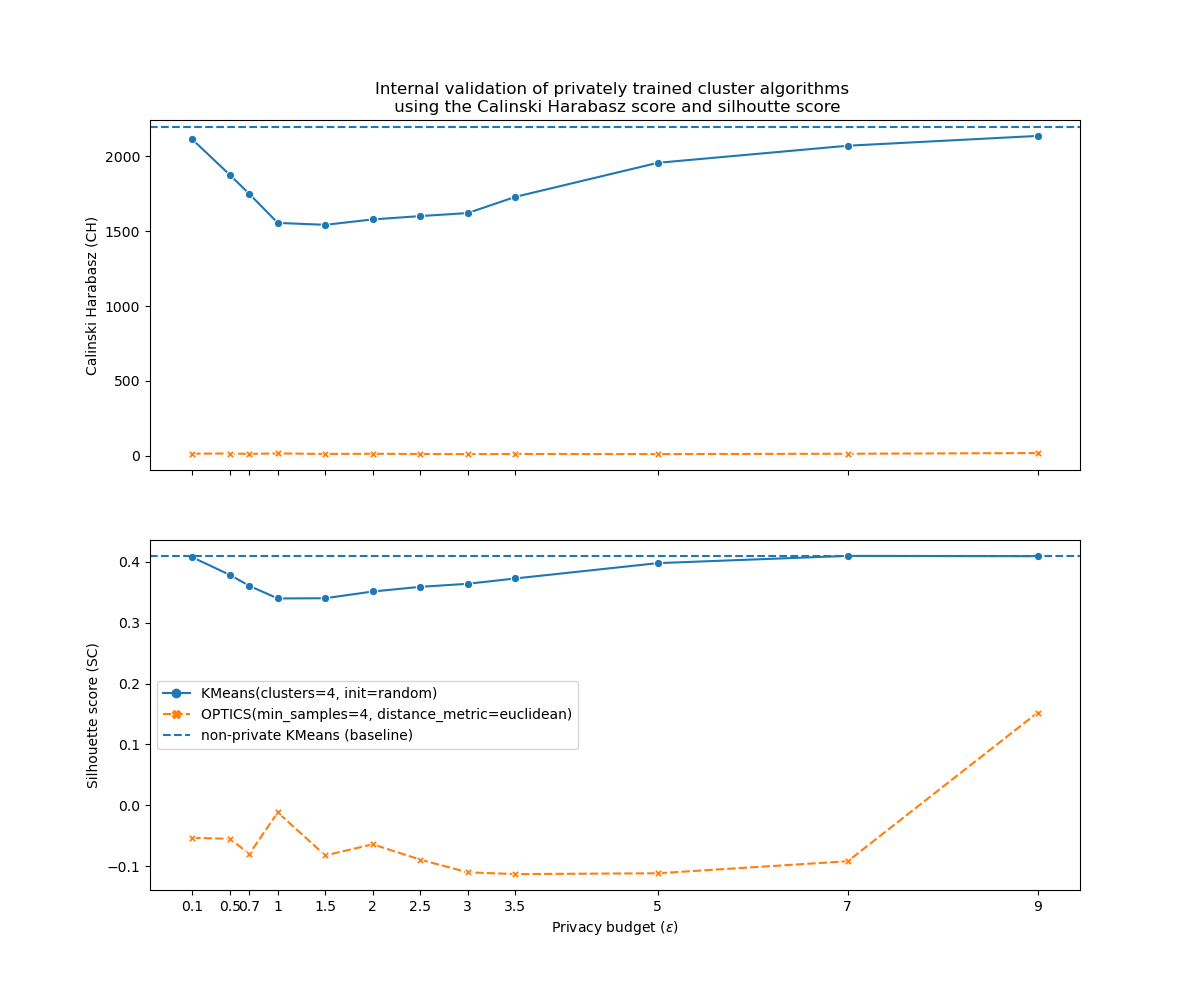
\includegraphics[width=1\textwidth]{Results/2d-piecewise/heart-dataset/ch-and-sc.png}
        \caption{Internal validation (CH/ SC) for the 2-dimensional data heart-dataset for piecewise mechanism}
        \label{fig:appendix-internal-validation-heart-dataset_comparison_2d-piecewise}
    \end{minipage}
\end{figure}



\begin{figure}[H]
    \caption{Internal validation for all mechanisms the 2-dimensional data seeds-dataset}
    \centering
    \begin{minipage}[c]{0.49\textwidth}
        %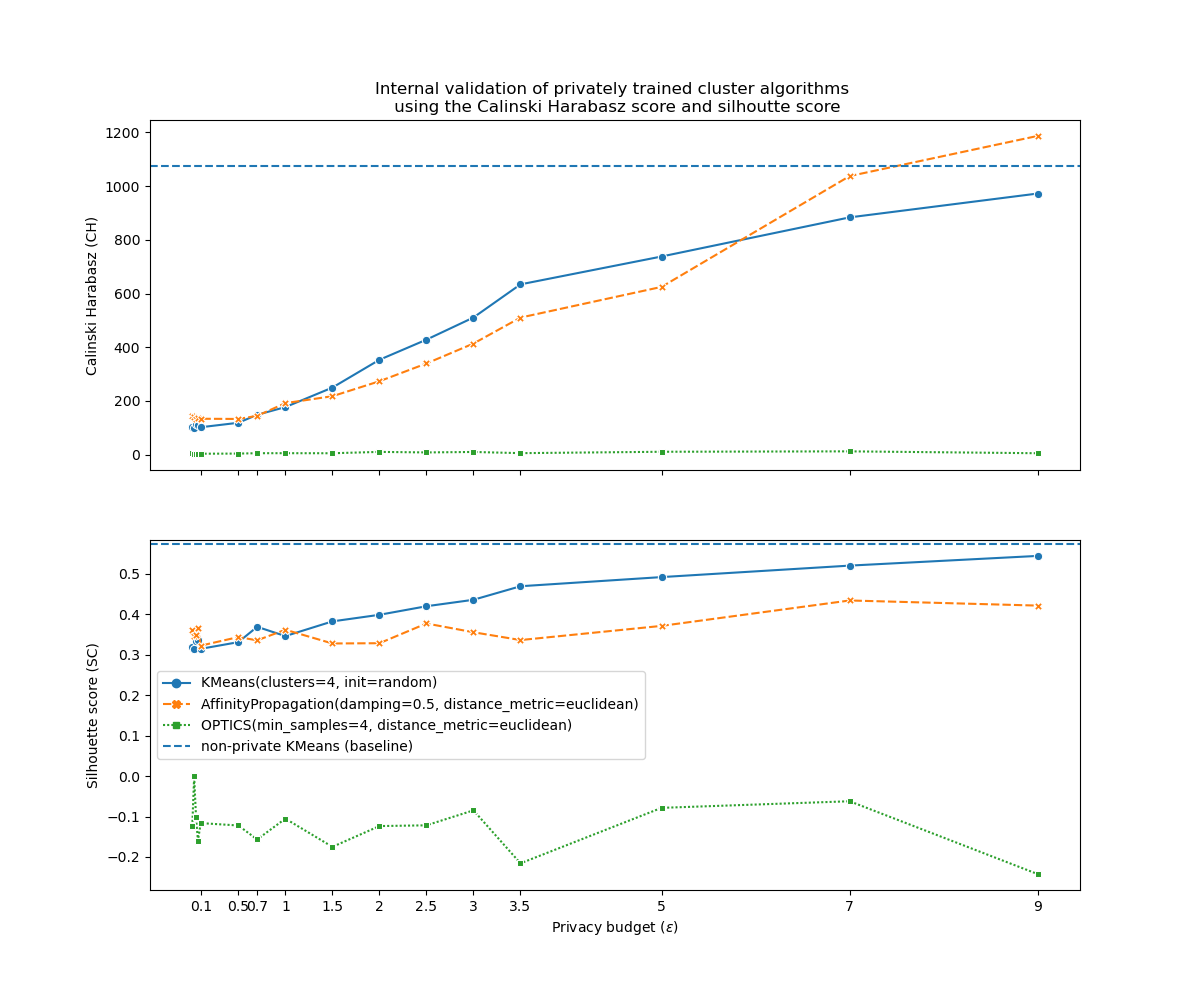
\includegraphics[width=1\textwidth]{Results/2d-laplace/seeds-dataset/ch-and-sc.png}
        \caption{Internal validation (CH/ SC) for the 2-dimensional data seeds-dataset for laplace.}
        \label{fig:appendix-internal-validation-seeds-dataset_comparison_2d-laplace}
    \end{minipage}
    \begin{minipage}[c]{0.49\textwidth}
        %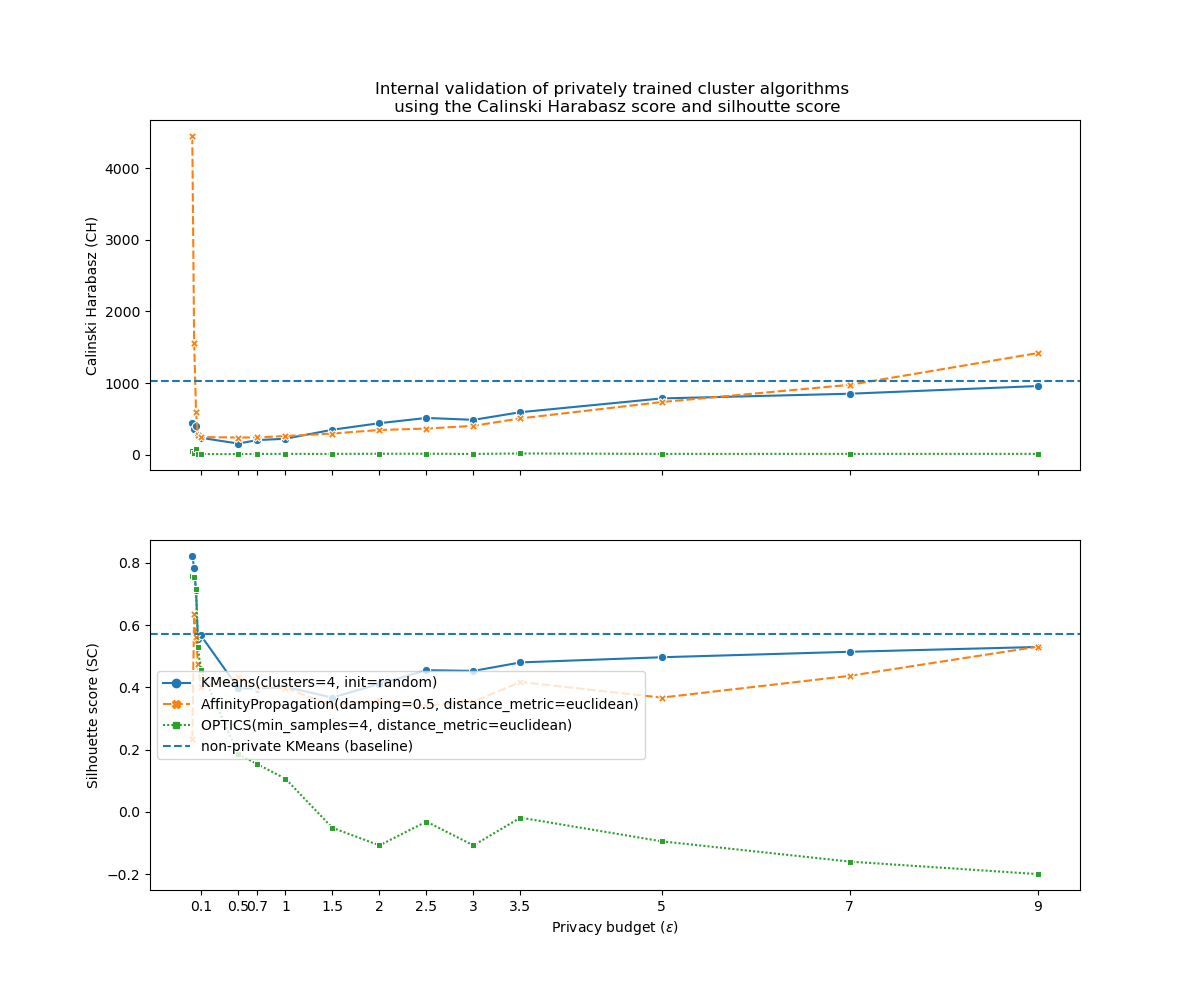
\includegraphics[width=1\textwidth]{Results/2d-laplace-truncated/seeds-dataset/ch-and-sc.png}
        \caption{Internal validation (CH/ SC) for the 2-dimensional data seeds-dataset for laplace with truncation.}
        \label{fig:appendix-internal-validation-seeds-dataset_comparison_2d-laplace-truncated}
    \end{minipage}
    \begin{minipage}[c]{0.49\textwidth}
        %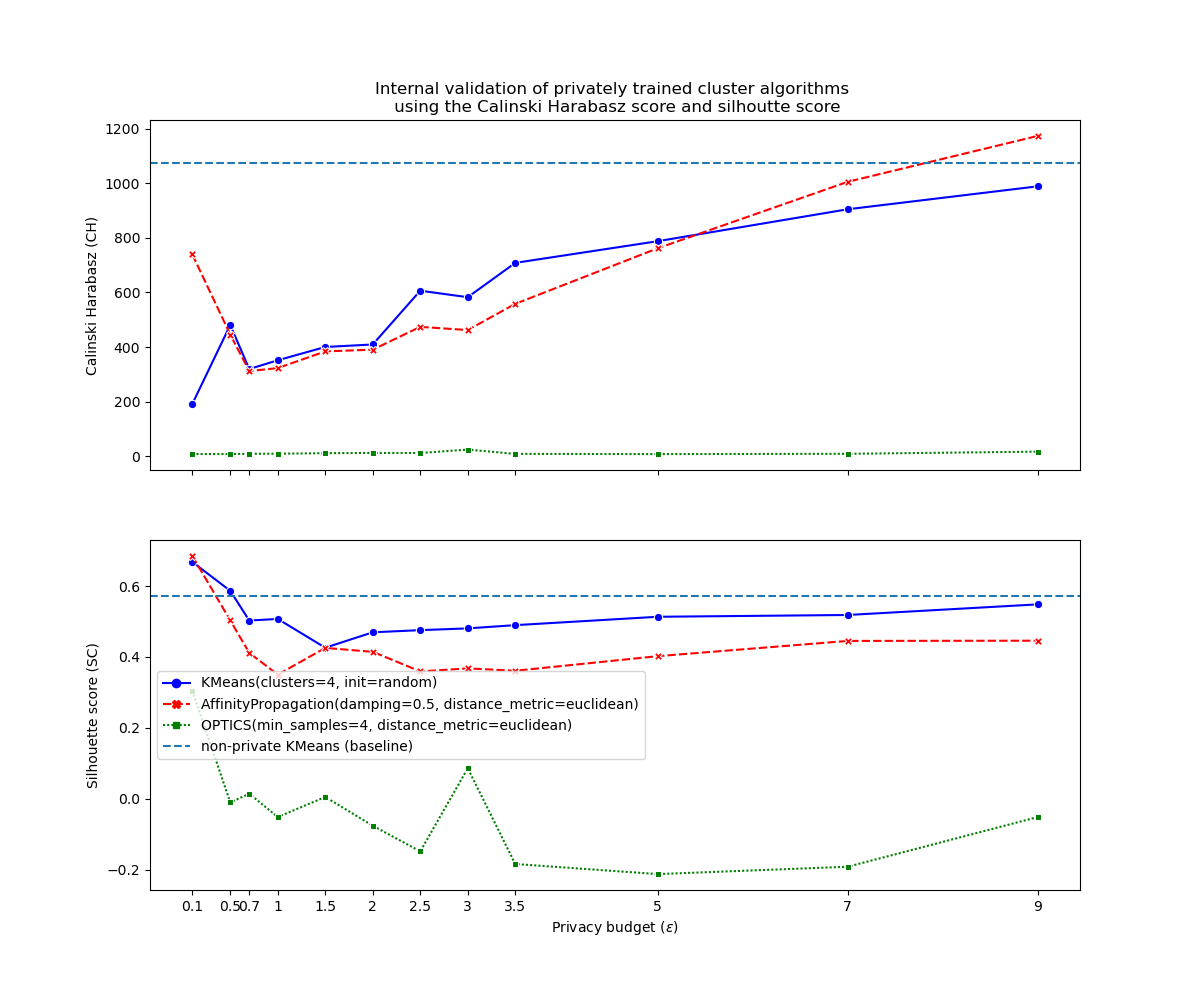
\includegraphics[width=1\textwidth]{Results/2d-laplace-optimal-truncated/seeds-dataset/ch-and-sc.png}
        \caption{Internal validation (CH/ SC) for the 2-dimensional data seeds-dataset for laplace with optimal truncation}
        \label{fig:appendix-internal-validation-seeds-dataset_comparison_2d-laplace-optimal-truncated}
    \end{minipage}
    \begin{minipage}[c]{0.49\textwidth}
        %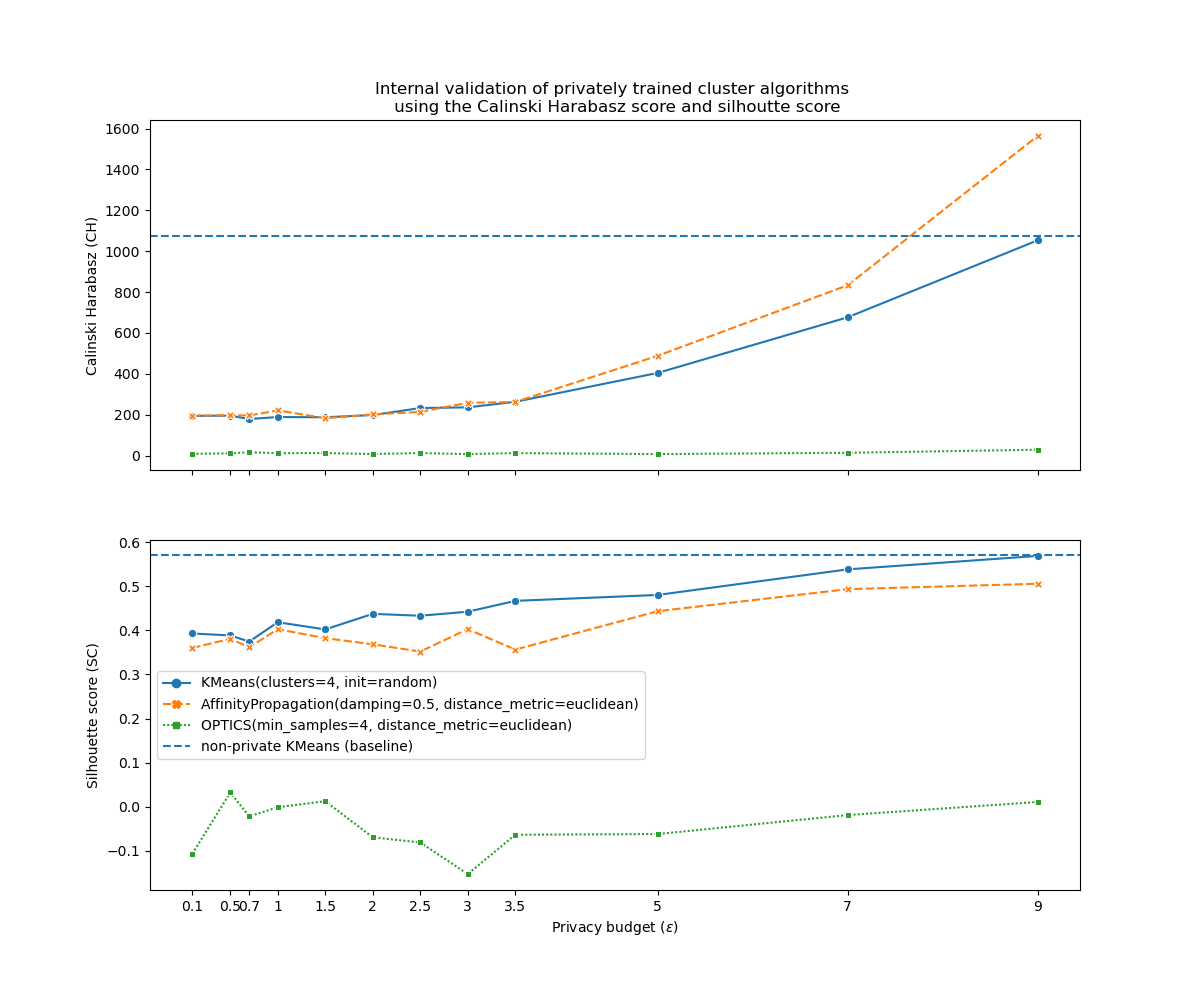
\includegraphics[width=1\textwidth]{Results/2d-piecewise/seeds-dataset/ch-and-sc.png}
        \caption{Internal validation (CH/ SC) for the 2-dimensional data seeds-dataset for piecewise mechanism}
        \label{fig:appendix-internal-validation-seeds-dataset_comparison_2d-piecewise}
    \end{minipage}
\end{figure}

\subsection{3-Dimensional data}

\mycomment{\begin{figure}[H]
        \caption{External validation for all mechanisms the 3-dimensional data seeds-dataset}
        \centering
        \begin{minipage}[c]{0.49\textwidth}
            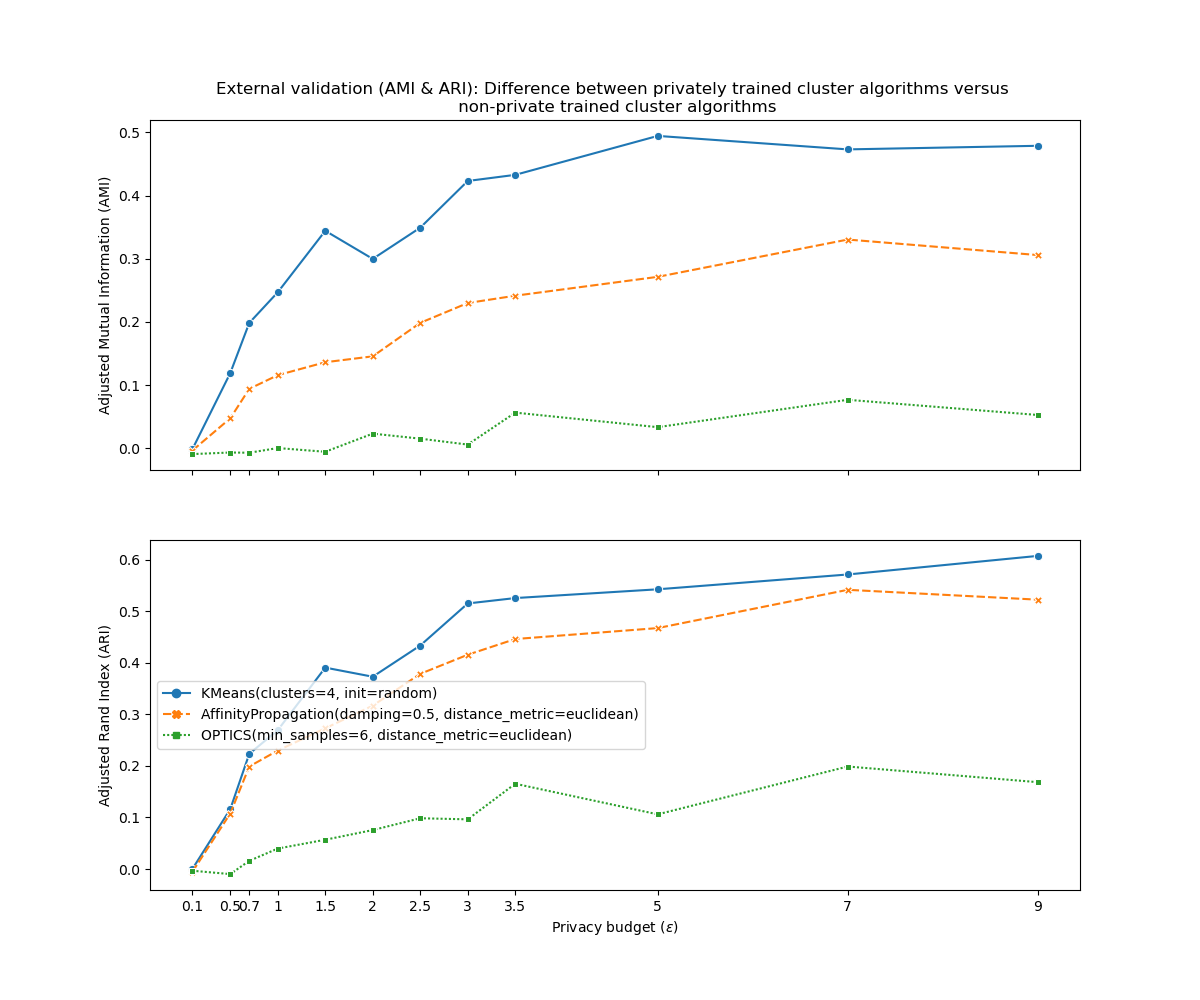
\includegraphics[width=1\textwidth]{Results/3d-laplace/seeds-dataset/ami-and-ari.png}
            \caption{External validation (ARI/ AMI) for the 3-dimensional data seeds-dataset for laplace.}
            \label{fig:appendix-external-validation-seeds-dataset_comparison_3d-laplace}
        \end{minipage}
        \begin{minipage}[c]{0.49\textwidth}
            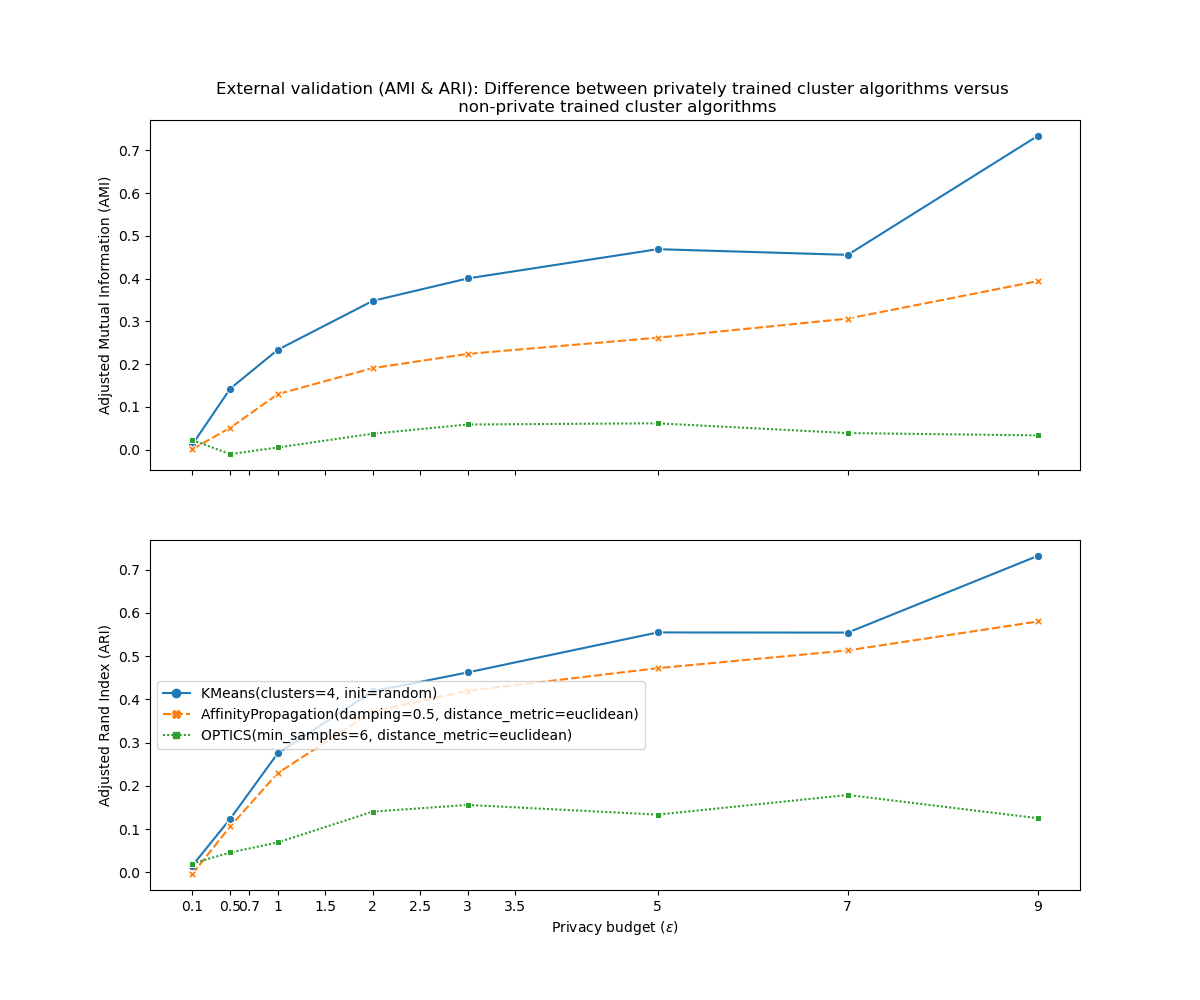
\includegraphics[width=1\textwidth]{Results/3d-laplace-truncated/seeds-dataset/ami-and-ari.png}
            \caption{External validation (ARI/ AMI) for the 3-dimensional data seeds-dataset for laplace with truncation.}
            \label{fig:appendix-external-validation-seeds-dataset_comparison_3d-laplace-truncated}
        \end{minipage}
        \begin{minipage}[c]{0.49\textwidth}
            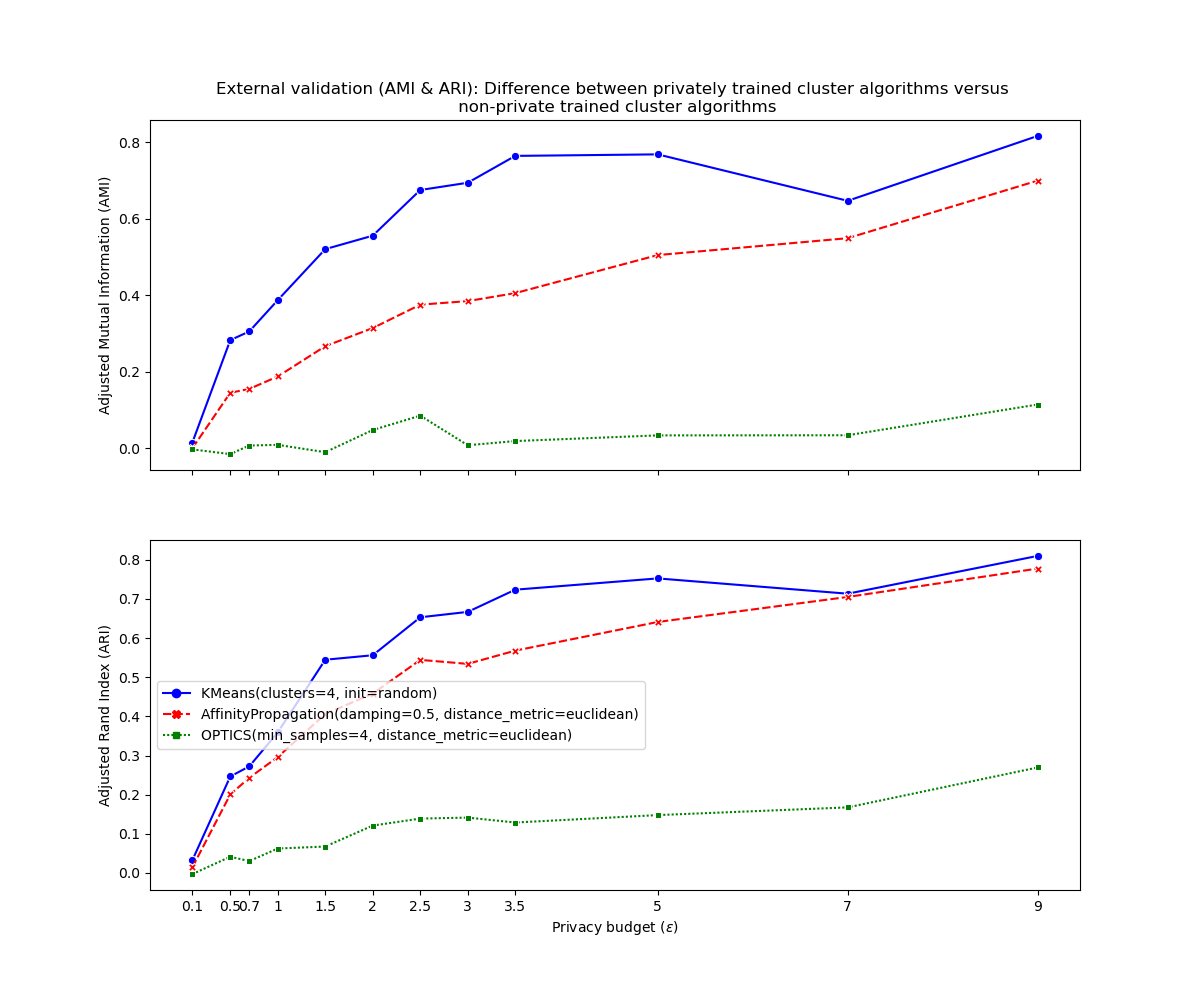
\includegraphics[width=1\textwidth]{Results/2d-laplace-optimal-truncated/seeds-dataset/ami-and-ari.png}
            \caption{External validation (ARI/ AMI) for the 2-dimensional data seeds-dataset for laplace with optimal truncation}
            \label{fig:appendix-external-validation-seeds-dataset_comparison_3d-laplace-optimal-truncated}
        \end{minipage}
        \begin{minipage}[c]{0.49\textwidth}
            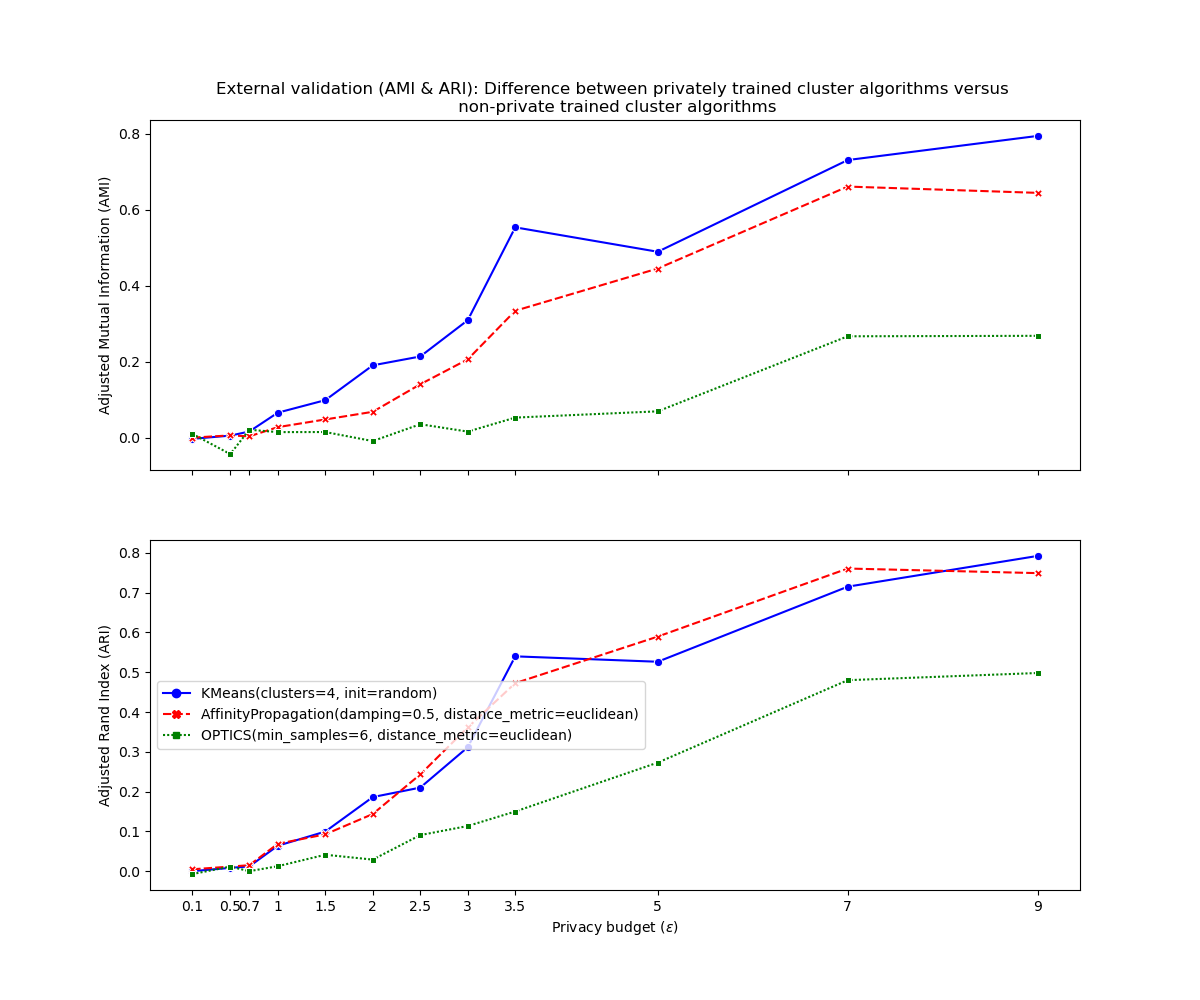
\includegraphics[width=1\textwidth]{Results/3d-piecewise/seeds-dataset/ami-and-ari.png}
            \caption{External validation (ARI/ AMI) for the 3-dimensional data seeds-dataset for piecewise mechanism}
            \label{fig:appendix-external-validation-seeds-dataset_comparison_3d-piecewise}
        \end{minipage}
    \end{figure}
}

\begin{figure}[H]
    \caption{Internal validation for all mechanisms the 3-dimensional data seeds-dataset}
    \centering
    \begin{minipage}[c]{0.49\textwidth}
        %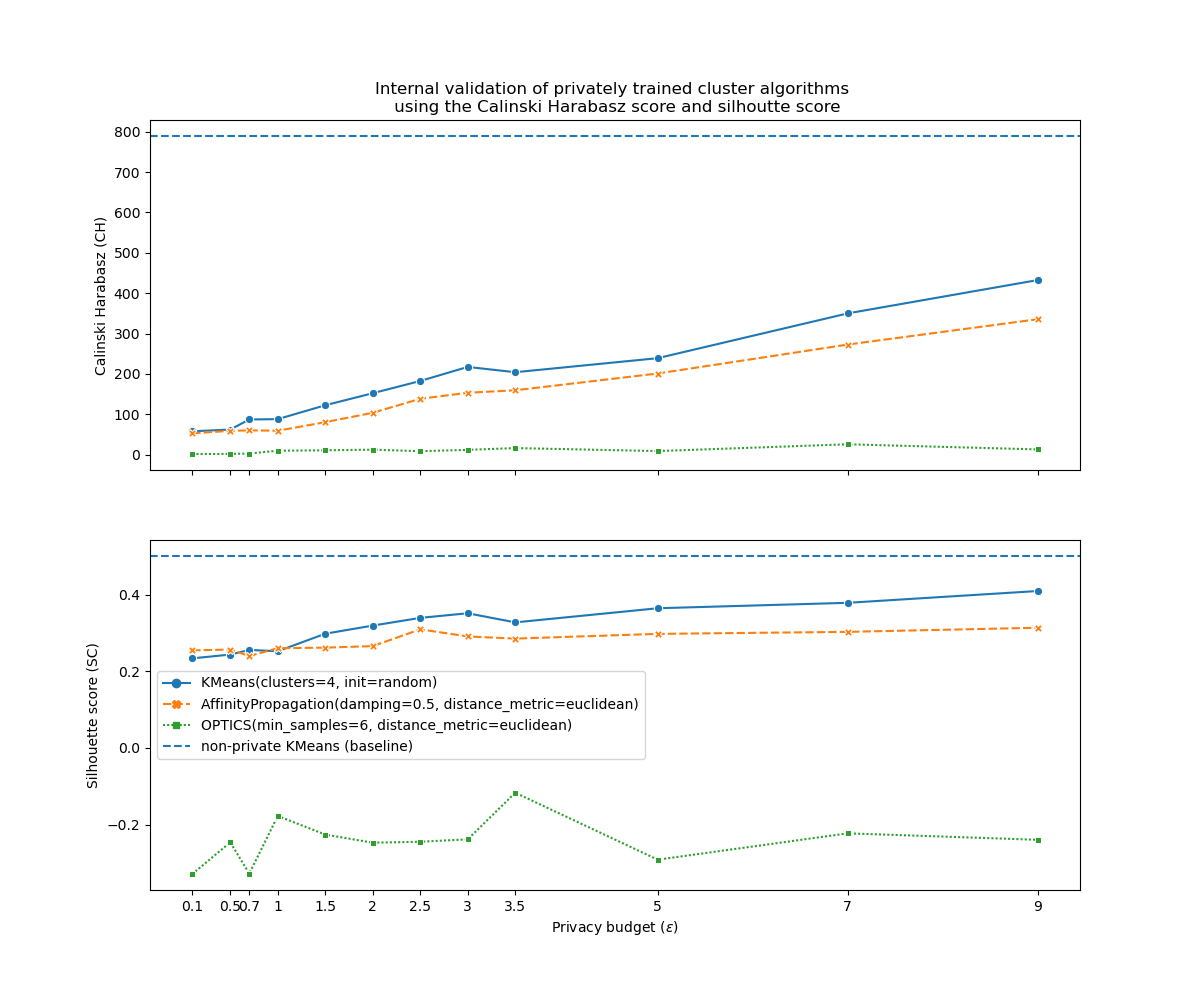
\includegraphics[width=1\textwidth]{Results/3d-laplace/seeds-dataset/ch-and-sc.png}
        \caption{Internal validation (CH/ SC) for the 3-dimensional data seeds-dataset for laplace.}
        \label{fig:appendix-internal-validation-seeds-dataset_comparison_3d-laplace}
    \end{minipage}
    \begin{minipage}[c]{0.49\textwidth}
        %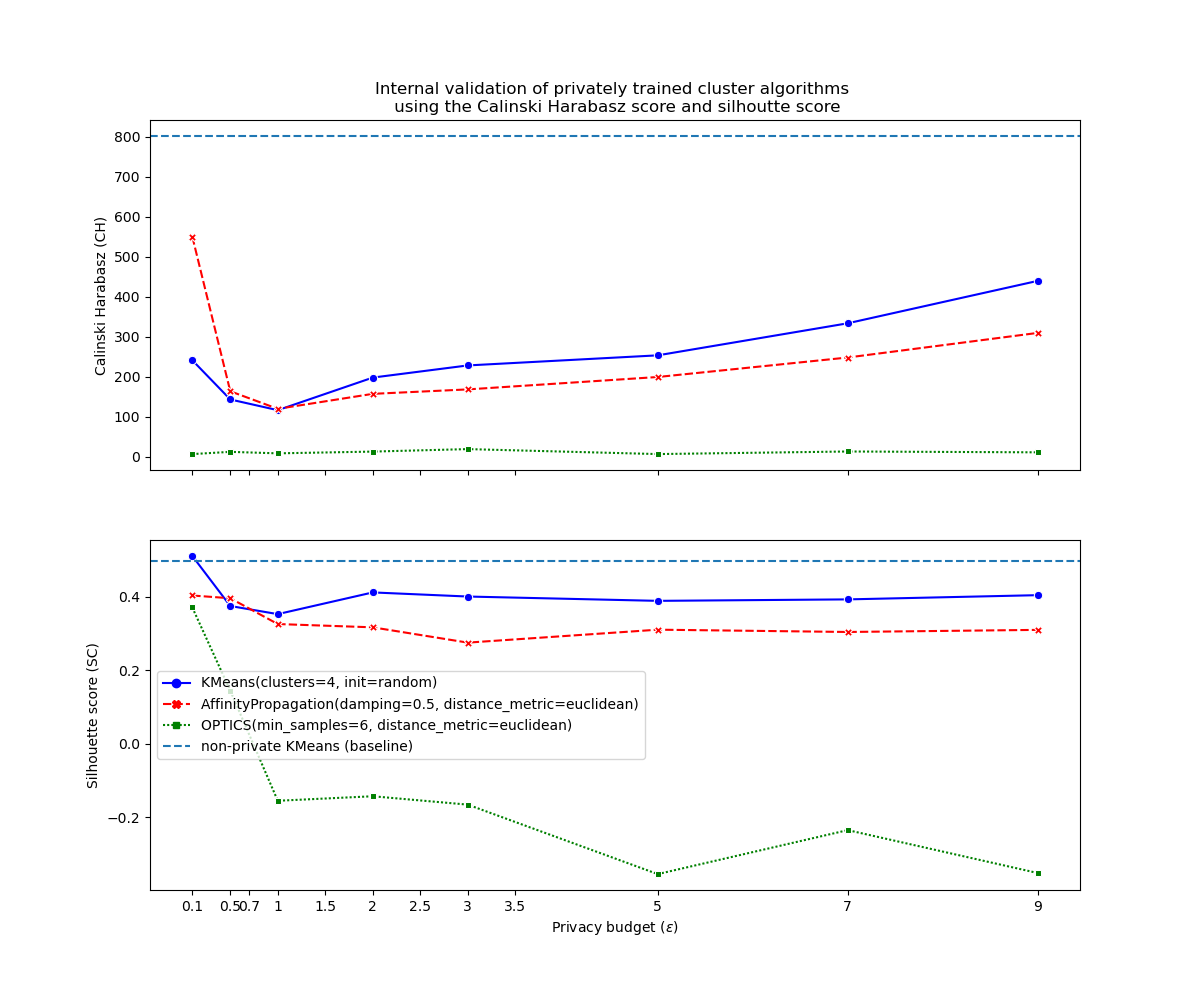
\includegraphics[width=1\textwidth]{Results/3d-laplace-truncated/seeds-dataset/ch-and-sc.png}
        \caption{Internal validation (CH/ SC) for the 3-dimensional data seeds-dataset for laplace with truncation.}
        \label{fig:appendix-internal-validation-seeds-dataset_comparison_3d-laplace-truncated}
    \end{minipage}
    \begin{minipage}[c]{0.49\textwidth}
        % 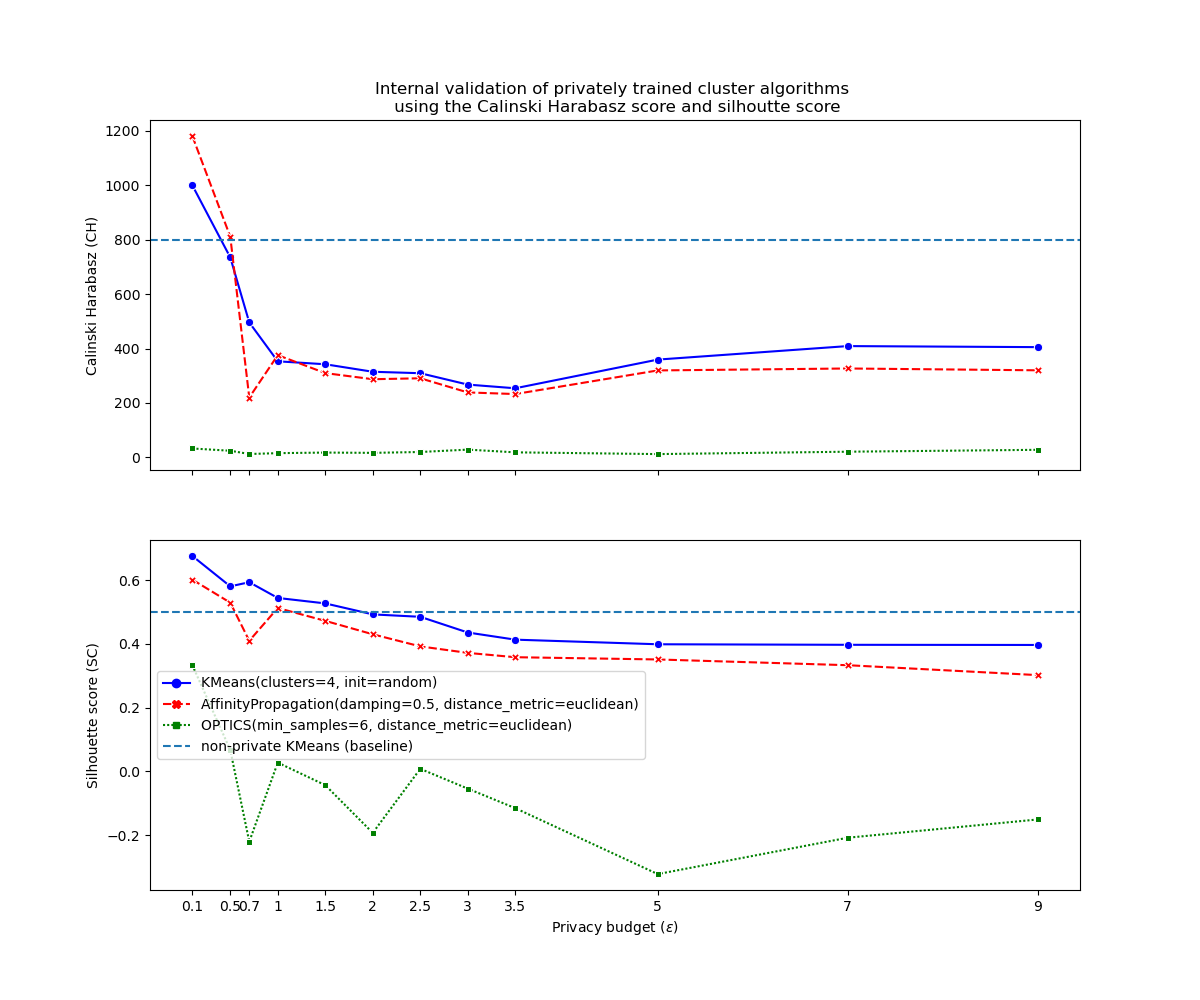
\includegraphics[width=1\textwidth]{Results/3d-laplace-optimal-truncated/seeds-dataset/ch-and-sc.png}
        \caption{Internal validation (CH/ SC) for the 3-dimensional data seeds-dataset for laplace with optimal truncation}
        \label{fig:appendix-internal-validation-seeds-dataset_comparison_3d-laplace-optimal-truncated}
    \end{minipage}
    \begin{minipage}[c]{0.49\textwidth}
        % 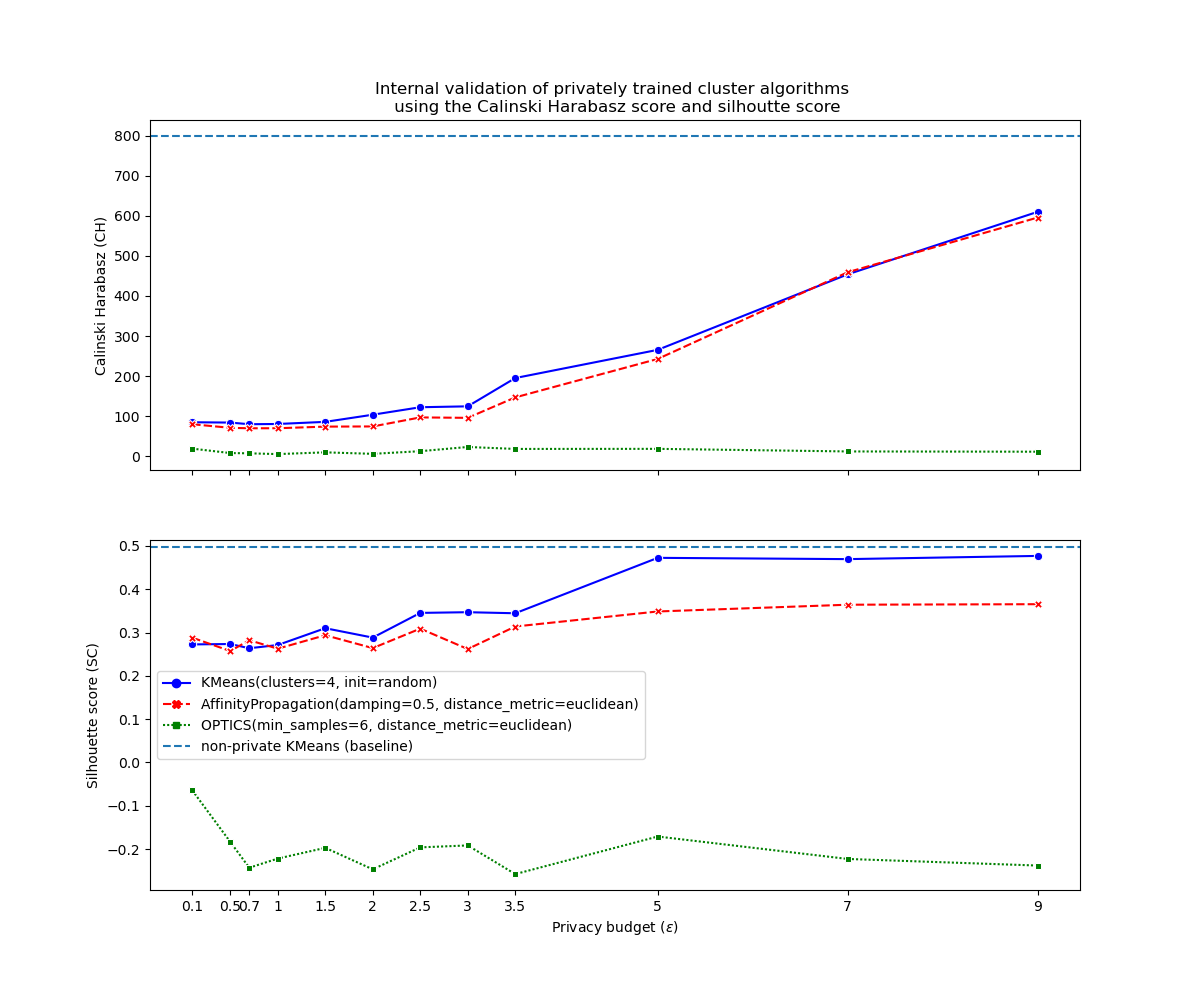
\includegraphics[width=1\textwidth]{Results/3d-piecewise/seeds-dataset/ch-and-sc.png}
        \caption{Internal validation (CH/ SC) for the 3-dimensional data seeds-dataset for piecewise mechanism}
        \label{fig:appendix-internal-validation-seeds-dataset_comparison_3d-piecewise}
    \end{minipage}
\end{figure}

\begin{figure}[H]
    \caption{Internal validation for all mechanisms the 3-dimensional data heart-dataset}
    \centering
    \begin{minipage}[c]{0.49\textwidth}
        %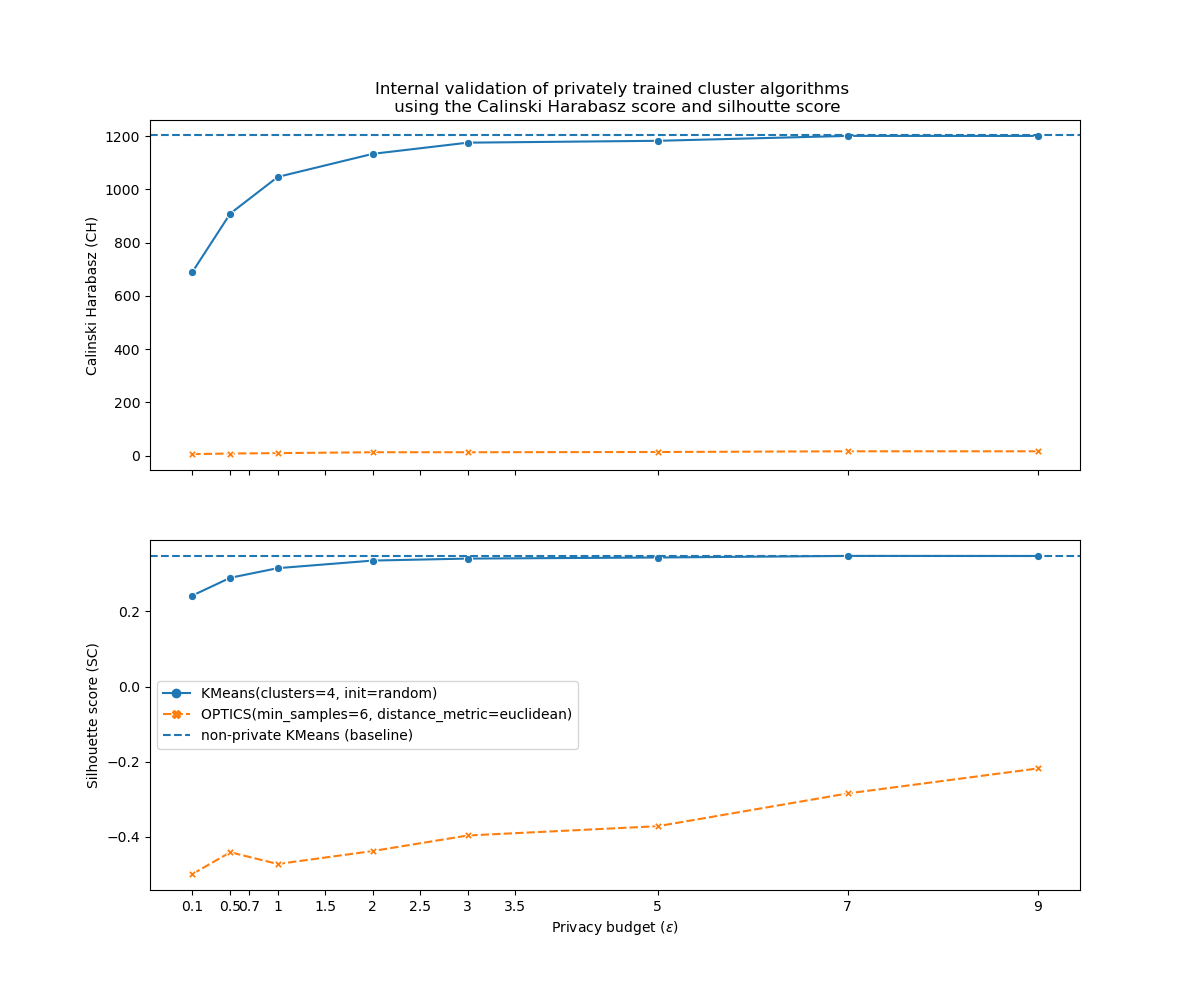
\includegraphics[width=1\textwidth]{Results/3d-laplace/heart-dataset/ch-and-sc.png}
        \caption{Internal validation (CH/ SC) for the 3-dimensional data heart-dataset for laplace.}
        \label{fig:appendix-internal-validation-heart-dataset_comparison_3d-laplace}
    \end{minipage}
    \begin{minipage}[c]{0.49\textwidth}
        %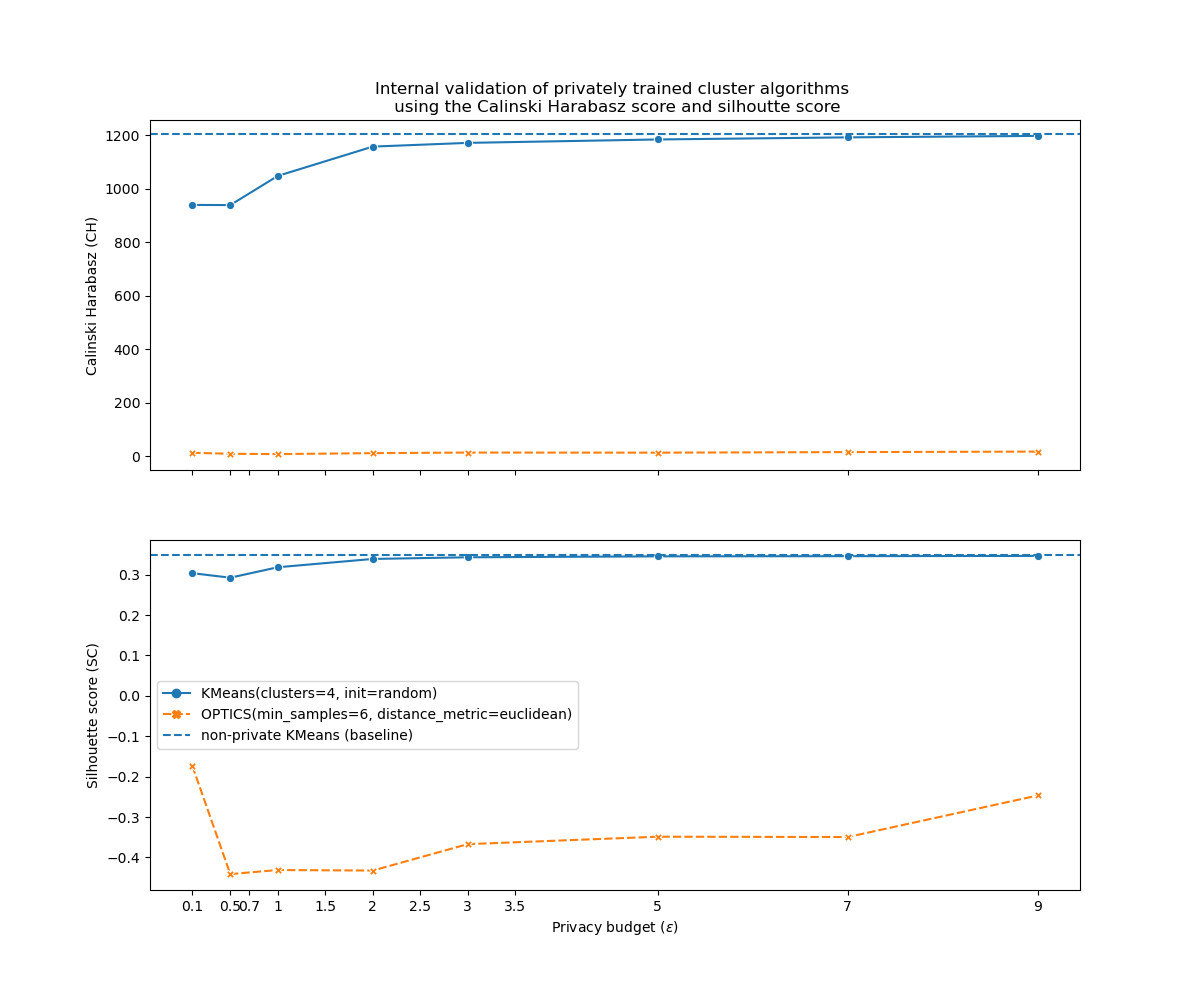
\includegraphics[width=1\textwidth]{Results/3d-laplace-truncated/heart-dataset/ch-and-sc.png}
        \caption{Internal validation (CH/ SC) for the 3-dimensional data heart-dataset for laplace with truncation.}
        \label{fig:appendix-internal-validation-heart-dataset_comparison_3d-laplace-truncated}
    \end{minipage}
    \begin{minipage}[c]{0.49\textwidth}
        %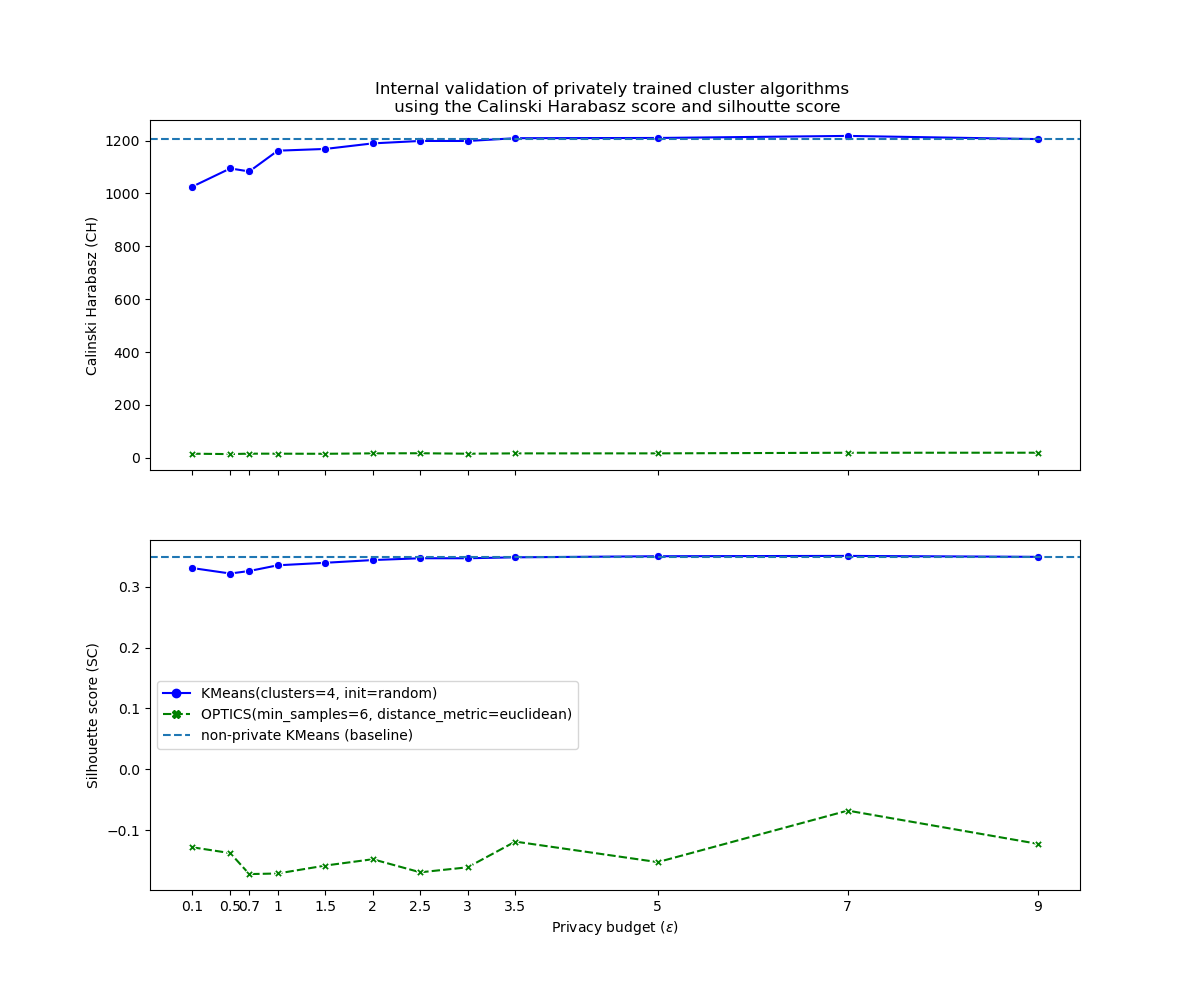
\includegraphics[width=1\textwidth]{Results/3d-laplace-optimal-truncated/heart-dataset/ch-and-sc.png}
        \caption{Internal validation (CH/ SC) for the 3-dimensional data heart-dataset for laplace with optimal truncation}
        \label{fig:appendix-internal-validation-heart-dataset_comparison_3d-laplace-optimal-truncated}
    \end{minipage}
    \begin{minipage}[c]{0.49\textwidth}
        %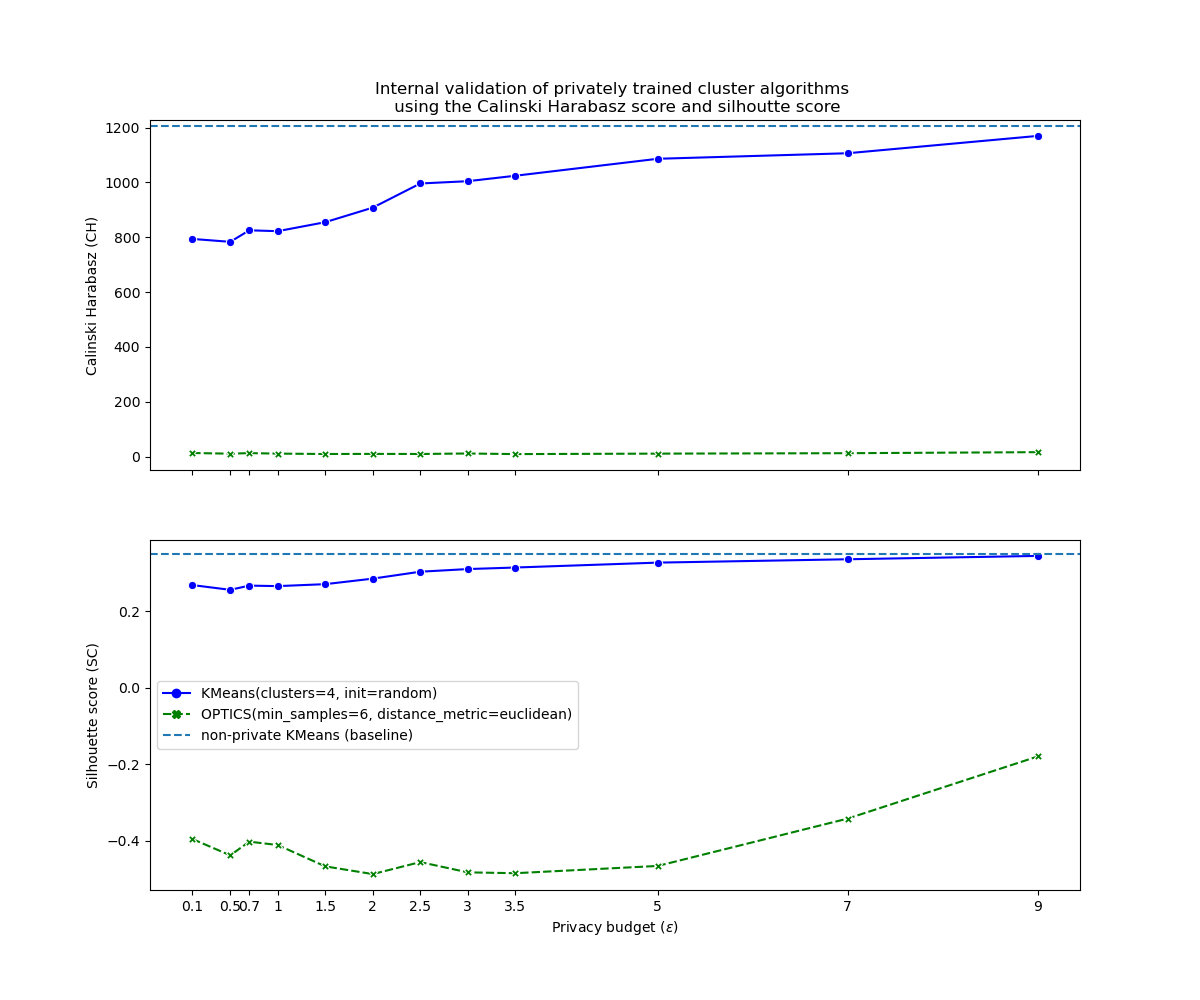
\includegraphics[width=1\textwidth]{Results/3d-piecewise/heart-dataset/ch-and-sc.png}
        \caption{Internal validation (CH/ SC) for the 3-dimensional data heart-dataset for piecewise mechanism}
        \label{fig:appendix-internal-validation-heart-dataset_comparison_3d-piecewise}
    \end{minipage}
\end{figure}
\subsection{n-Dimensional data}
\begin{figure}[H]
    \caption{Internal validation for all mechanisms the n-dimensional data seeds-dataset}
    \centering
    \begin{minipage}[c]{0.49\textwidth}
        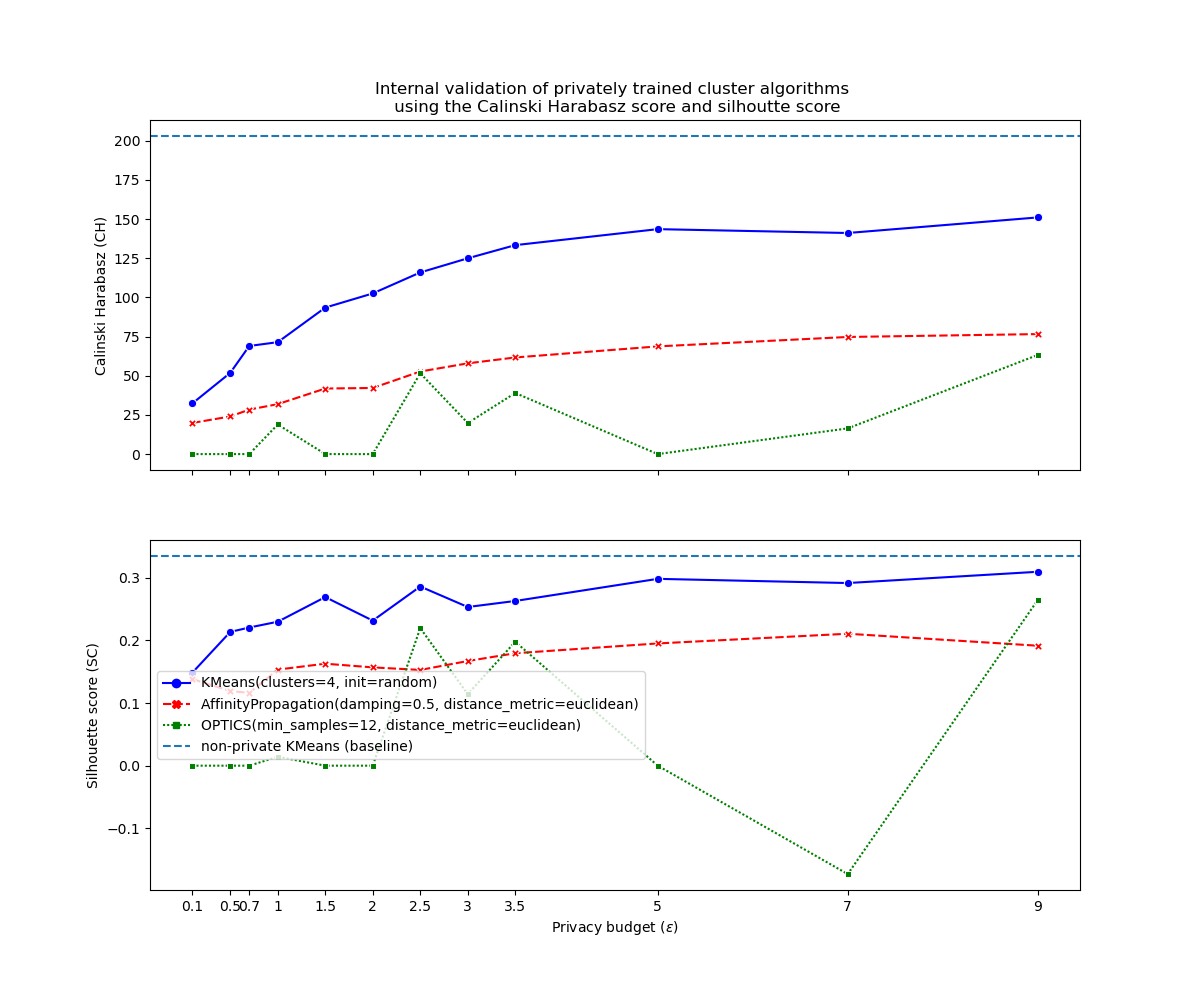
\includegraphics[width=1\textwidth]{Results/nd-laplace/seeds-dataset/ch-and-sc.png}
        \caption{Internal validation (CH/ SC) for the n-dimensional data seeds-dataset for laplace.}
        \label{fig:appendix-internal-validation-seeds-dataset_comparison_nd-laplace}
    \end{minipage}
    \begin{minipage}[c]{0.49\textwidth}
        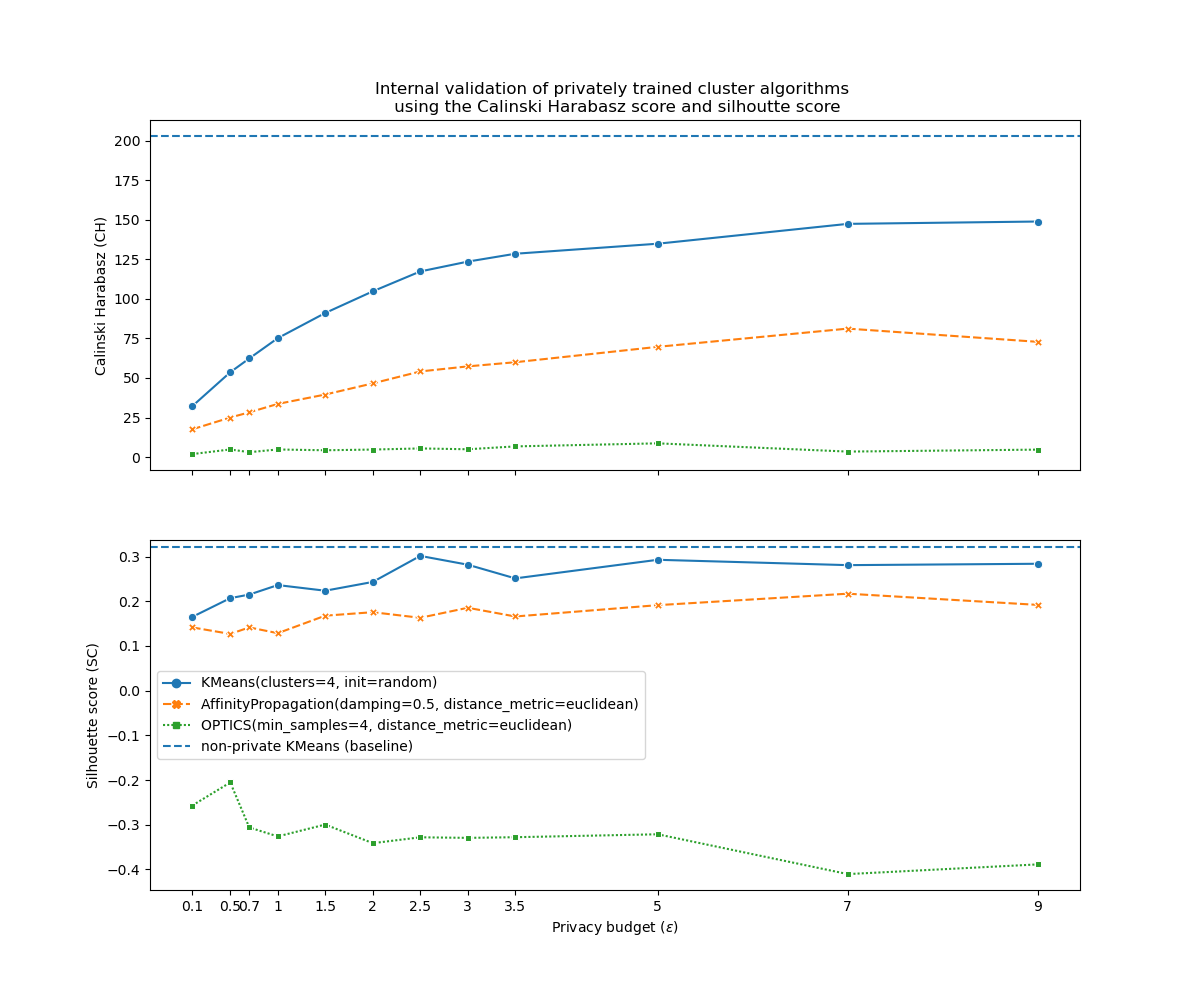
\includegraphics[width=1\textwidth]{Results/nd-laplace-truncated/seeds-dataset/ch-and-sc.png}
        \caption{Internal validation (CH/ SC) for the n-dimensional data seeds-dataset for laplace with truncation.}
        \label{fig:appendix-internal-validation-seeds-dataset_comparison_nd-laplace-truncated}
    \end{minipage}
    \begin{minipage}[c]{0.49\textwidth}
        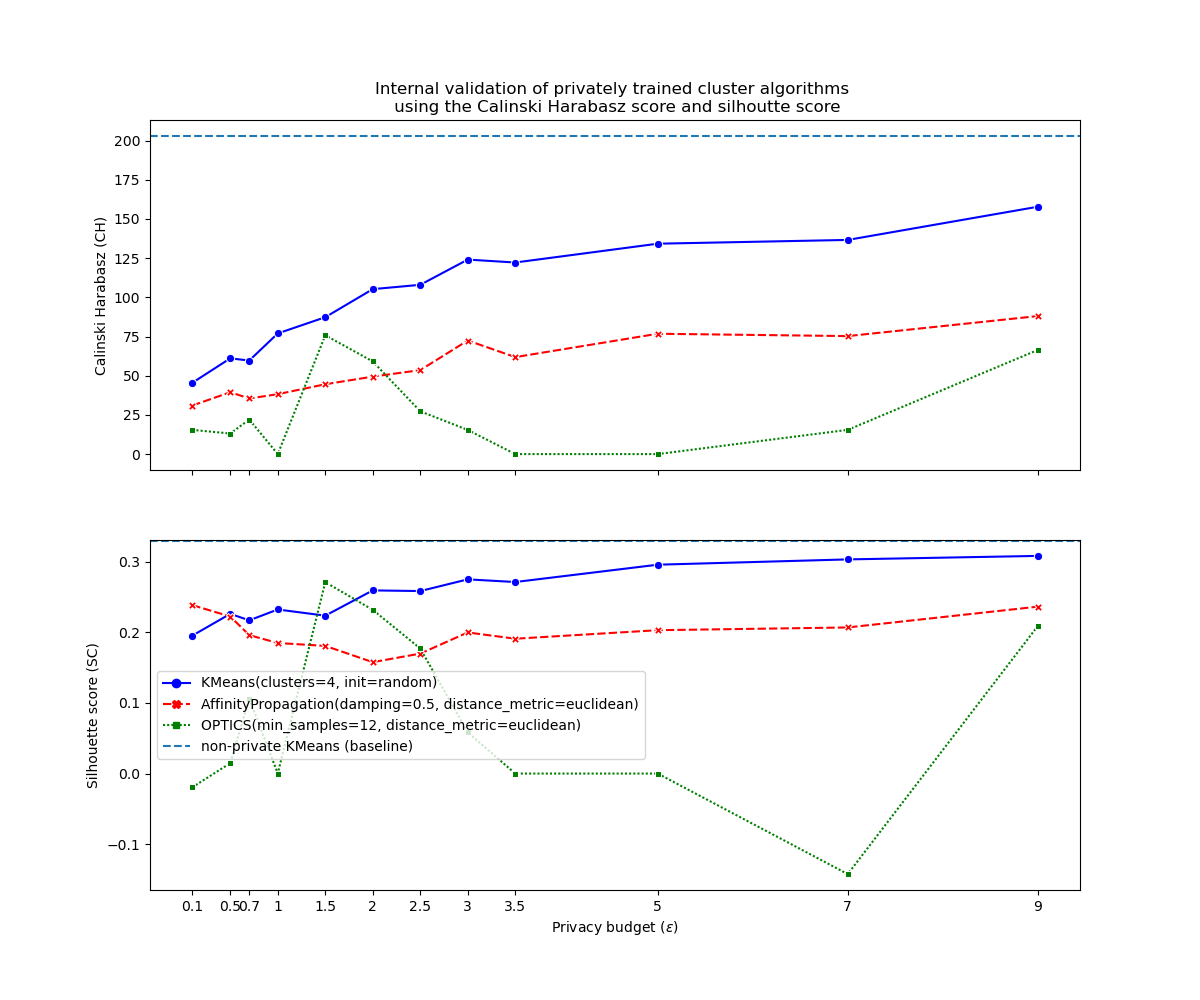
\includegraphics[width=1\textwidth]{Results/nd-laplace-optimal-truncated/seeds-dataset/ch-and-sc.png}
        \caption{Internal validation (CH/ SC) for the n-dimensional data seeds-dataset for laplace with optimal truncation}
        \label{fig:appendix-internal-validation-seeds-dataset_comparison_nd-laplace-optimal-truncated}
    \end{minipage}
    \begin{minipage}[c]{0.49\textwidth}
        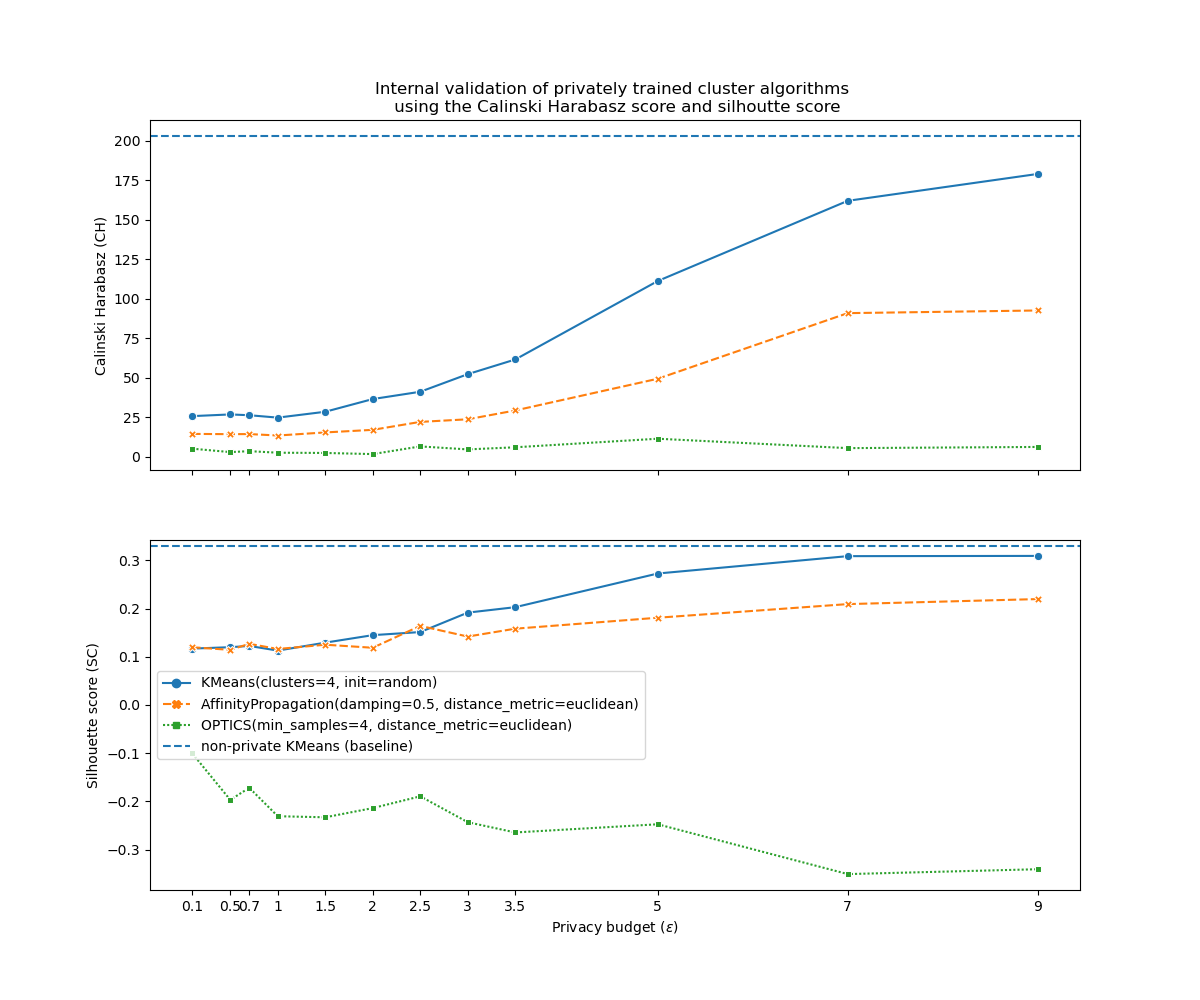
\includegraphics[width=1\textwidth]{Results/nd-piecewise/seeds-dataset/ch-and-sc.png}
        \caption{Internal validation (CH/ SC) for the n-dimensional data seeds-dataset for piecewise mechanism}
        \label{fig:appendix-internal-validation-seeds-dataset_comparison_nd-piecewise}
    \end{minipage}
\end{figure}
\begin{figure}[H]
    \caption{Internal validation for all mechanisms the n-dimensional data heart-dataset}
    \centering
    \begin{minipage}[c]{0.49\textwidth}
        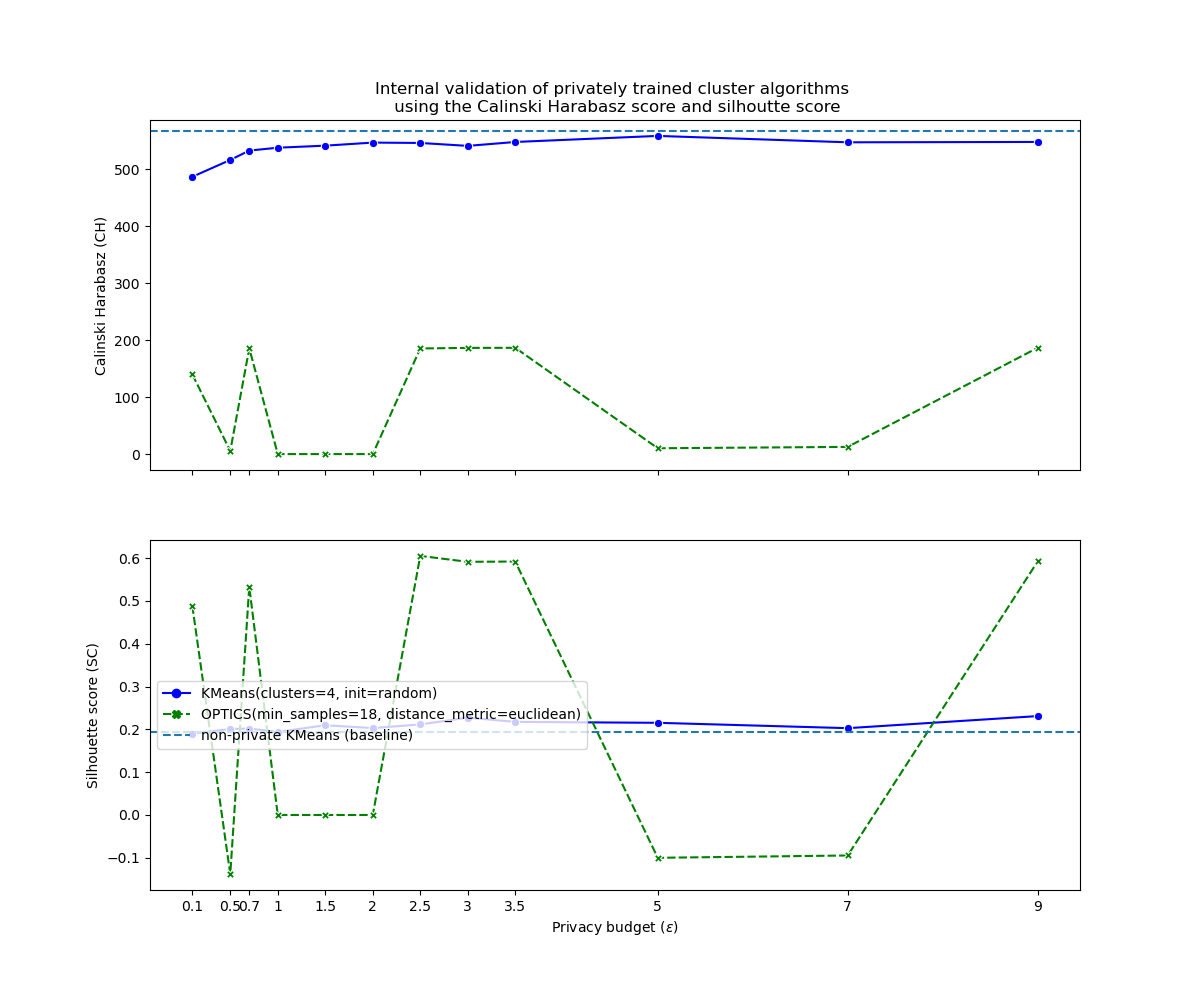
\includegraphics[width=1\textwidth]{Results/nd-laplace/heart-dataset/ch-and-sc.png}
        \caption{Internal validation (CH/ SC) for the n-dimensional data heart-dataset for laplace.}
        \label{fig:appendix-internal-validation-heart-dataset_comparison_nd-laplace}
    \end{minipage}
    \begin{minipage}[c]{0.49\textwidth}
        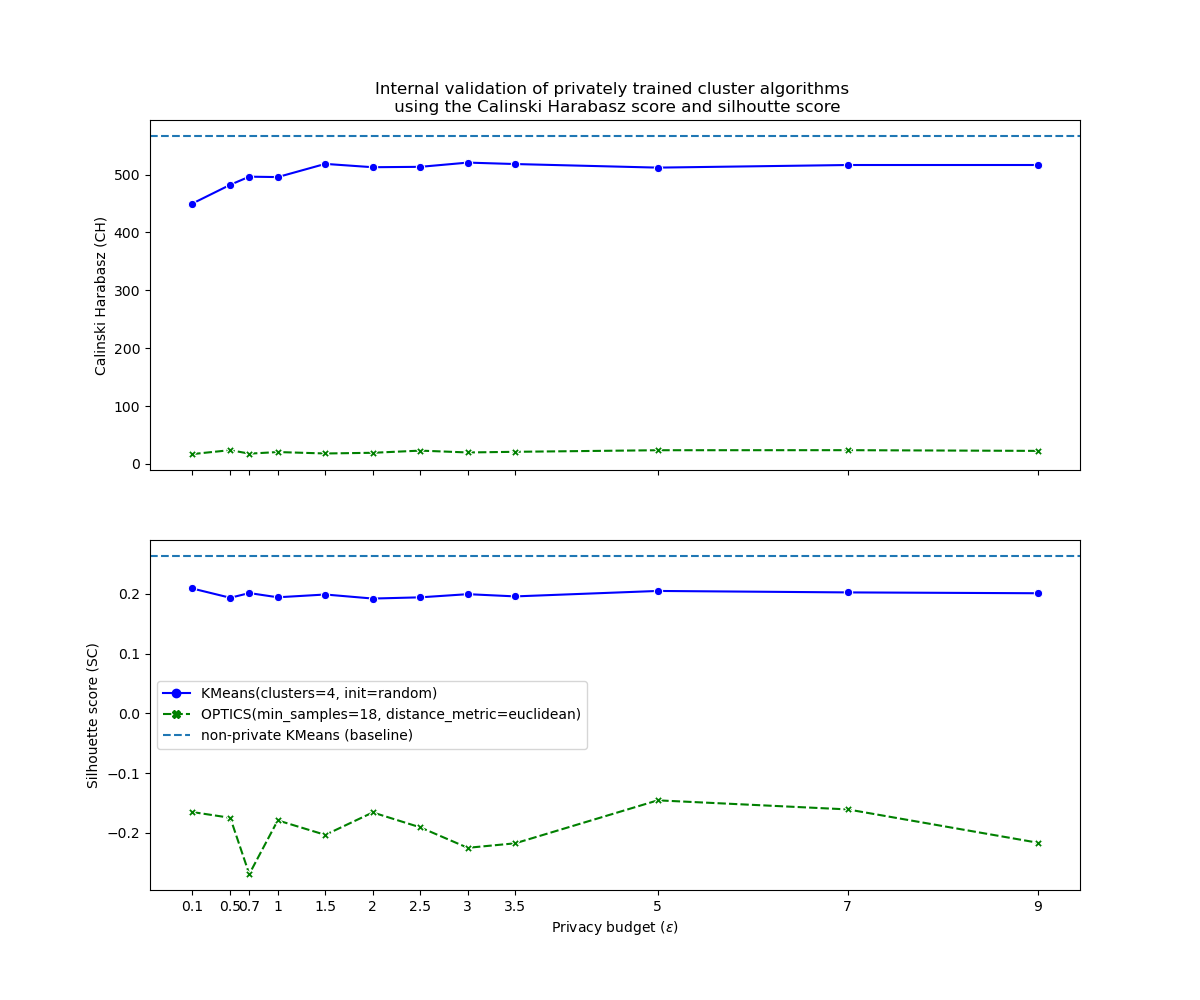
\includegraphics[width=1\textwidth]{Results/nd-laplace-truncated/heart-dataset/ch-and-sc.png}
        \caption{Internal validation (CH/ SC) for the n-dimensional data heart-dataset for laplace with truncation.}
        \label{fig:appendix-internal-validation-heart-dataset_comparison_nd-laplace-truncated}
    \end{minipage}
    \begin{minipage}[c]{0.49\textwidth}
        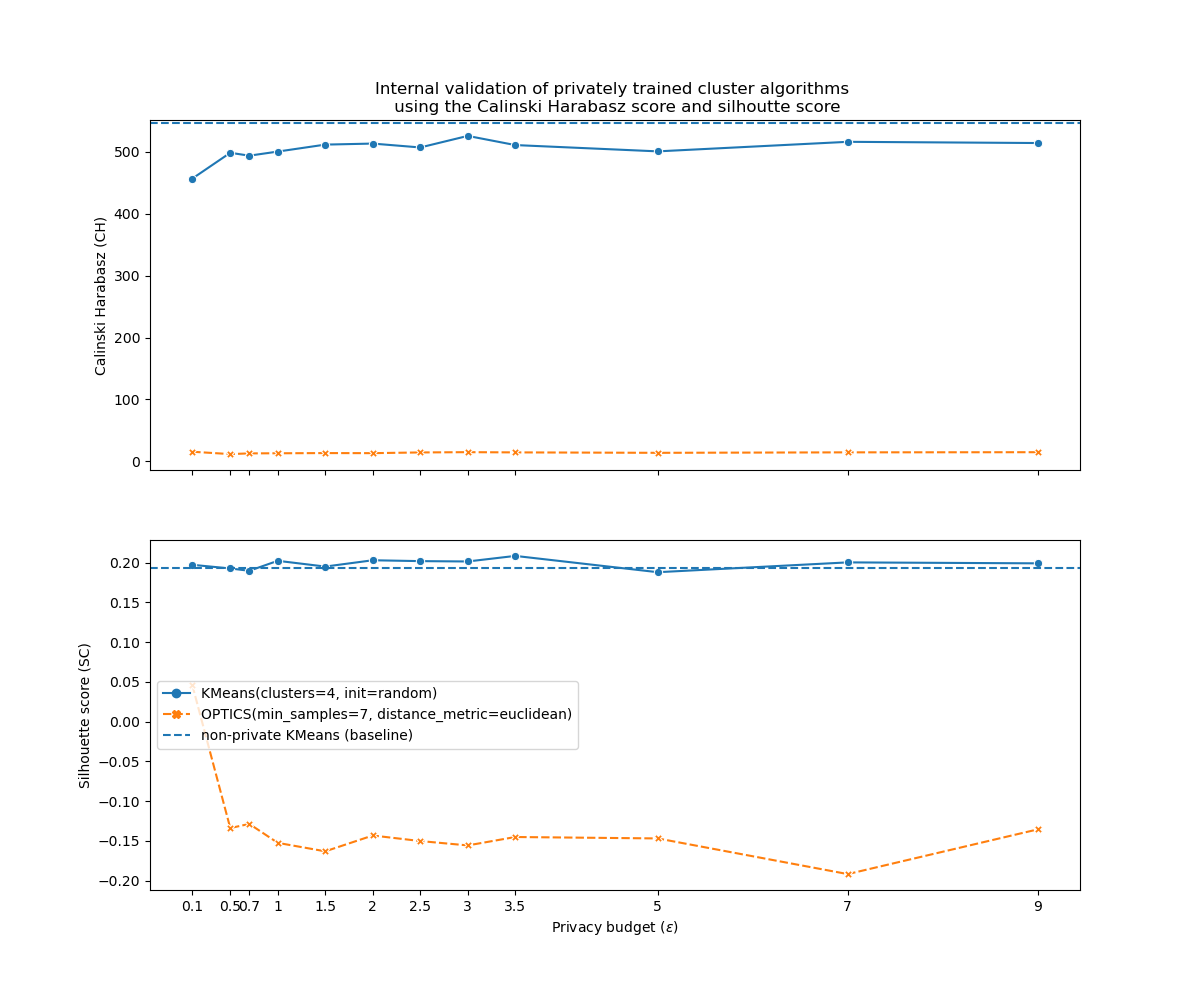
\includegraphics[width=1\textwidth]{Results/nd-laplace-optimal-truncated/heart-dataset/ch-and-sc.png}
        \caption{Internal validation (CH/ SC) for the n-dimensional data heart-dataset for laplace with optimal truncation}
        \label{fig:appendix-internal-validation-heart-dataset_comparison_nd-laplace-optimal-truncated}
    \end{minipage}
    \begin{minipage}[c]{0.49\textwidth}
        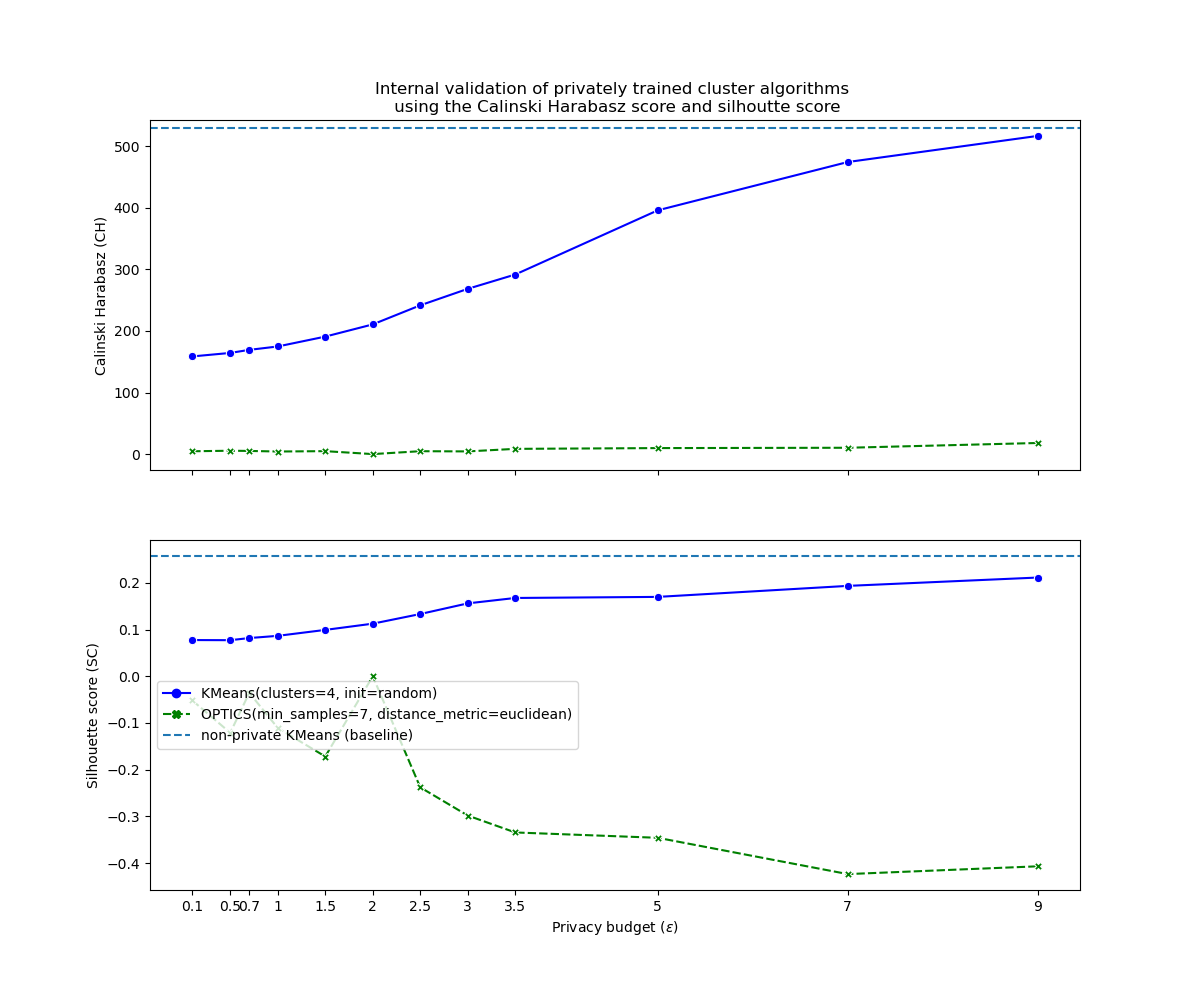
\includegraphics[width=1\textwidth]{Results/nd-piecewise/heart-dataset/ch-and-sc.png}
        \caption{Internal validation (CH/ SC) for the n-dimensional data heart-dataset for piecewise mechanism}
        \label{fig:appendix-internal-validation-heart-dataset_comparison_nd-piecewise}
    \end{minipage}
\end{figure}
\section{Mechanism utility} \label{appendix:results-mechanism-utility}
\subsection{2-Dimensional data}
\begin{figure}[H]
    \centering
    \begin{minipage}[c]{0.8\textwidth}
        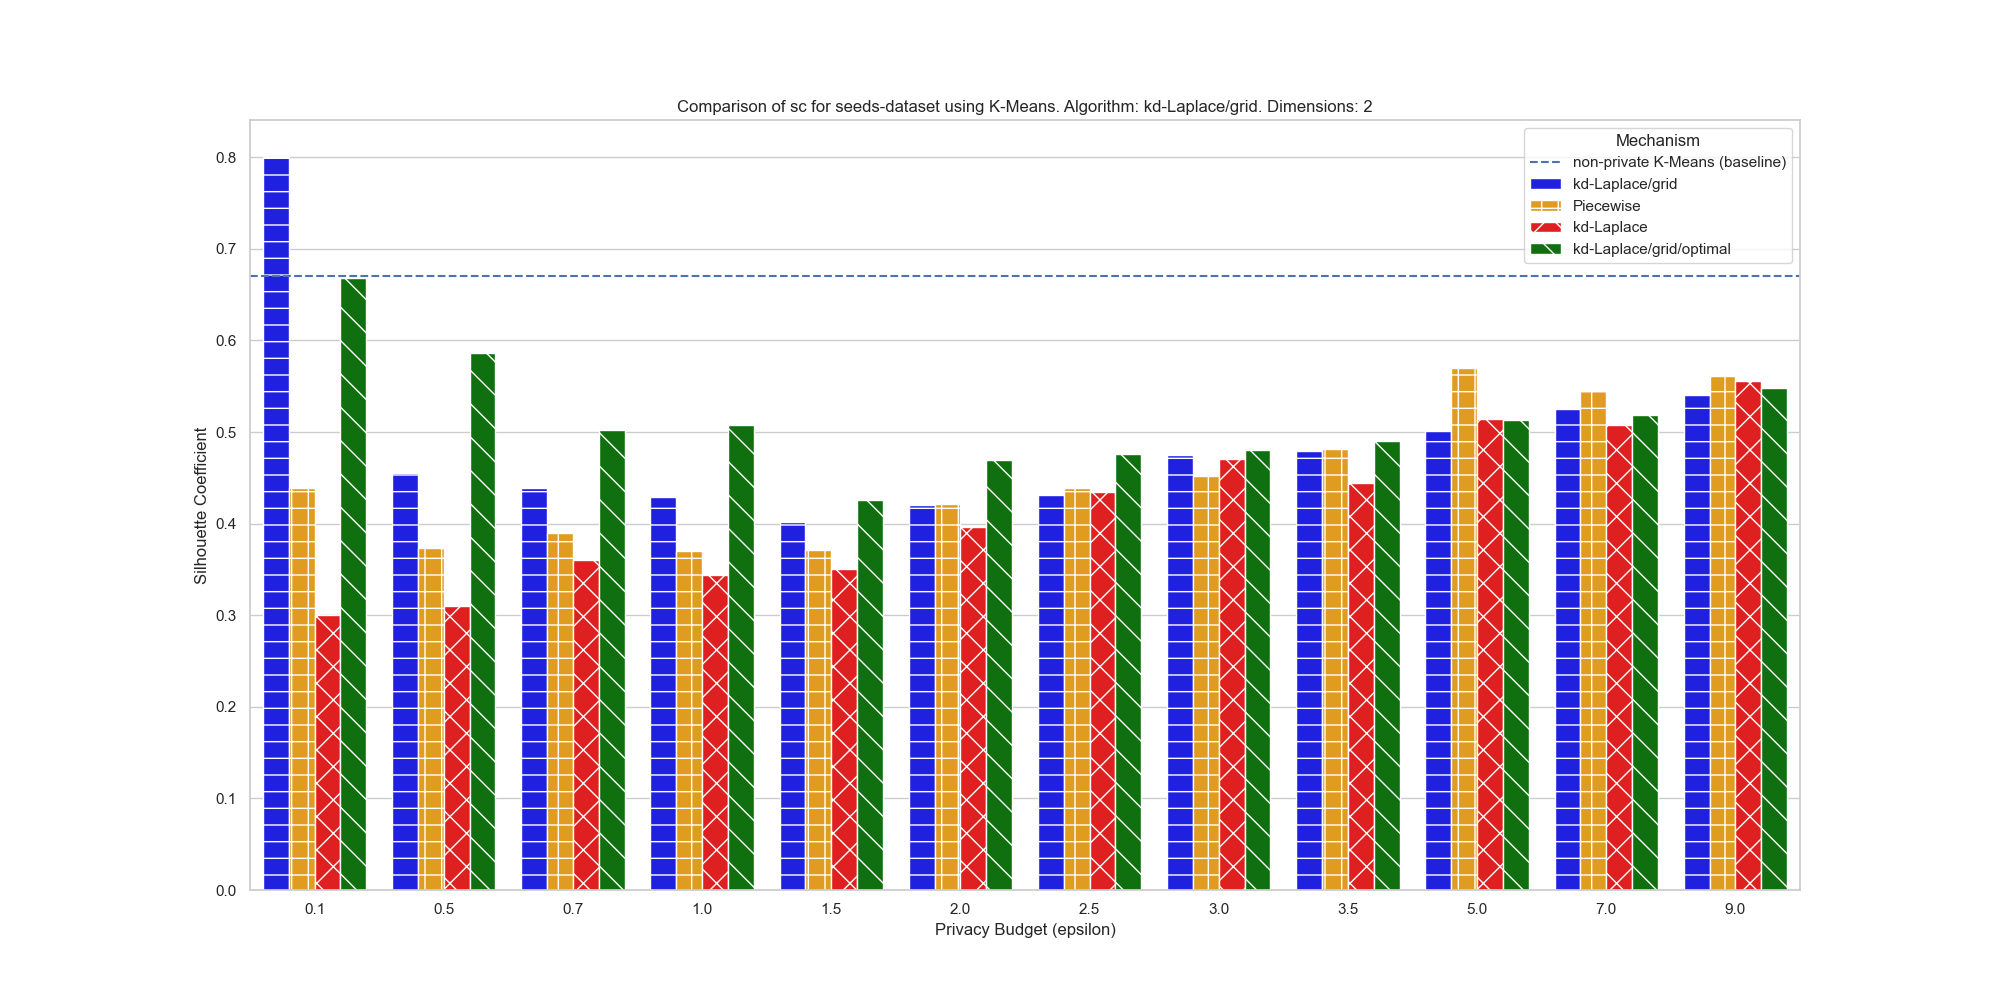
\includegraphics[width=1\textwidth]{Results/RQ1/seeds-dataset/sc_seeds-dataset_comparison.png}
        \caption{Silhouette score comparison for the 2D seeds-dataset}
        \label{fig:appendix-sc_seeds-dataset_comparison_2d}
    \end{minipage}
    \begin{minipage}[c]{0.8\textwidth}
        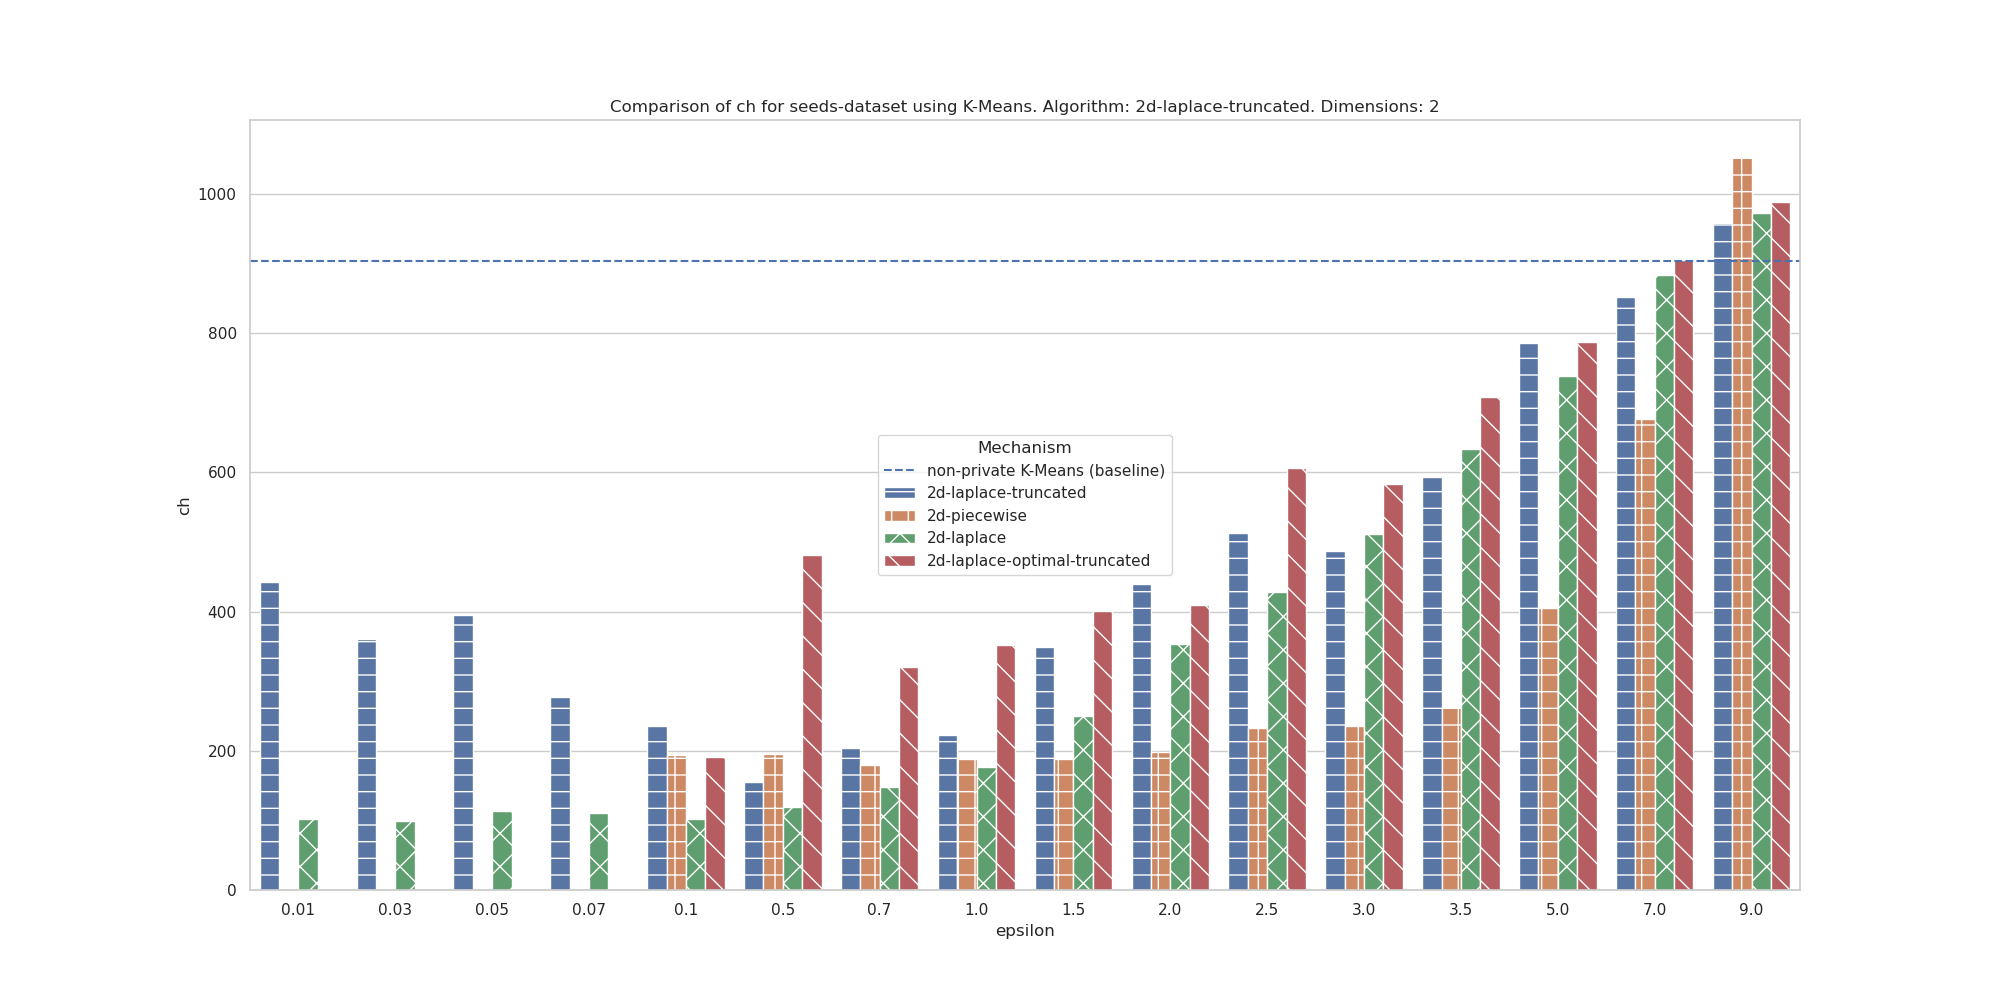
\includegraphics[width=1\textwidth]{Results/RQ1/seeds-dataset/ch_seeds-dataset_comparison.png}
        \caption{Calinski Harabasz score comparison for the 2D seeds-dataset}
        \label{fig:appendix-ch_seeds-dataset_comparison_2d}
    \end{minipage}

\end{figure}
\begin{figure}[H]
    \centering
    \begin{minipage}[c]{0.8\textwidth}
        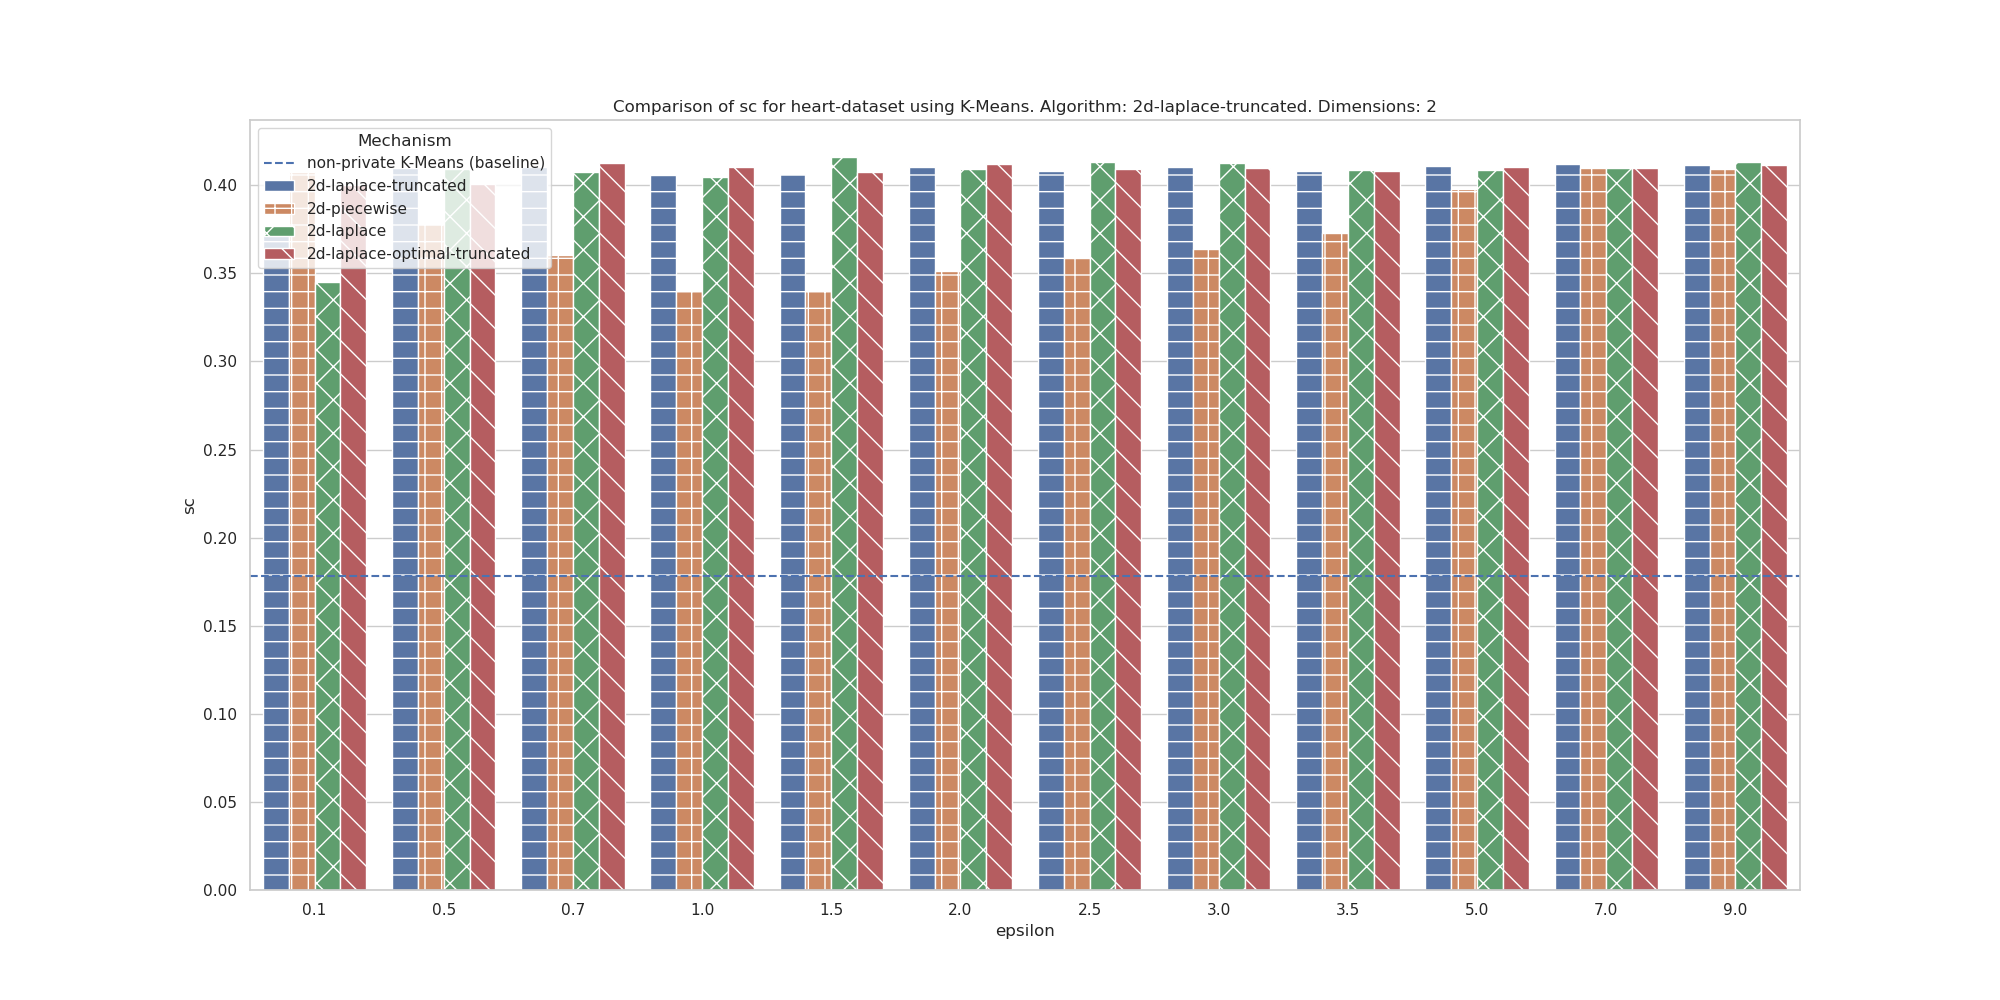
\includegraphics[width=1\textwidth]{Results/RQ1/heart-dataset/sc_heart-dataset_comparison.png}
        \caption{Silhouette score comparison for the 2D heart-dataset}
        \label{fig:appendix-sc_heart-dataset_comparison_2d}
    \end{minipage}
    \begin{minipage}[c]{0.8\textwidth}
        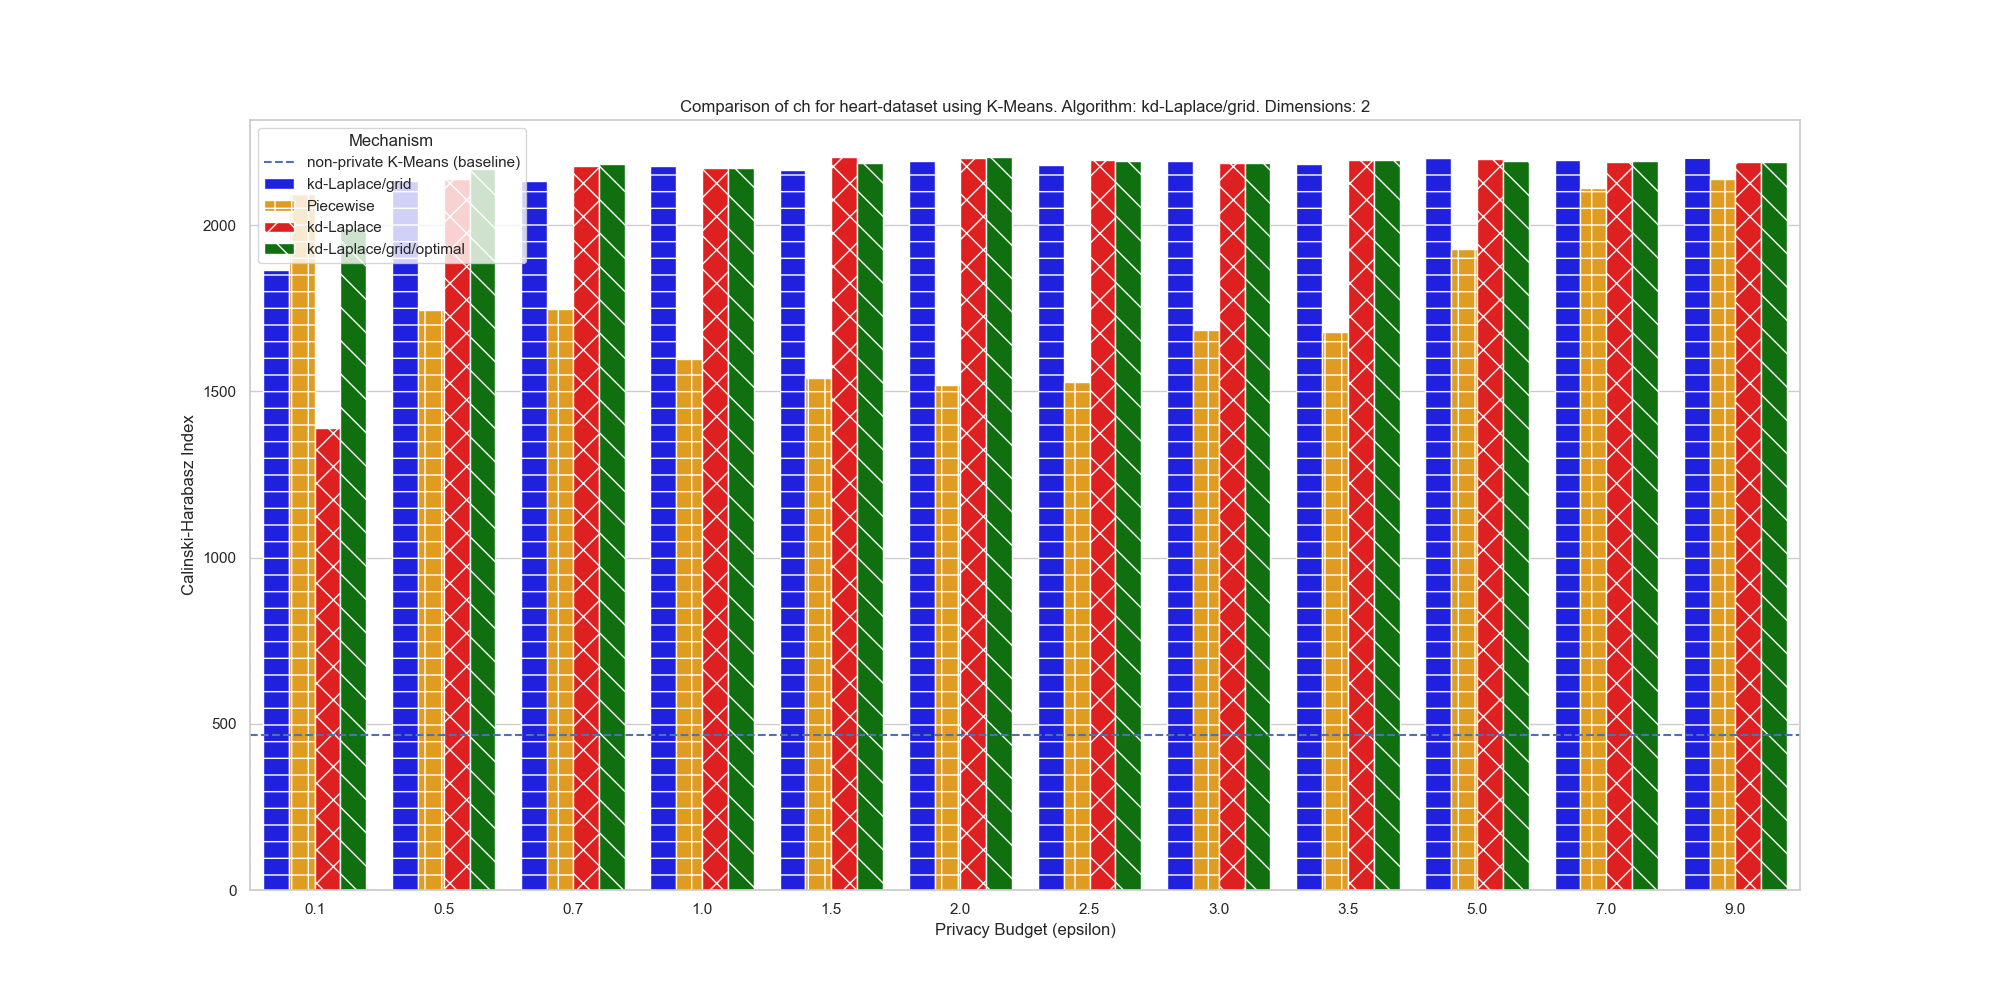
\includegraphics[width=1\textwidth]{Results/RQ1/heart-dataset/ch_heart-dataset_comparison.png}
        \caption{Calinski Harabasz score comparison for the 2D heart-dataset}
        \label{fig:appendix-ch_heart-dataset_comparison_2d}
    \end{minipage}

\end{figure}
\subsection{3-Dimensional data}
\begin{figure}[H]
    \centering
    \begin{minipage}[c]{0.8\textwidth}
        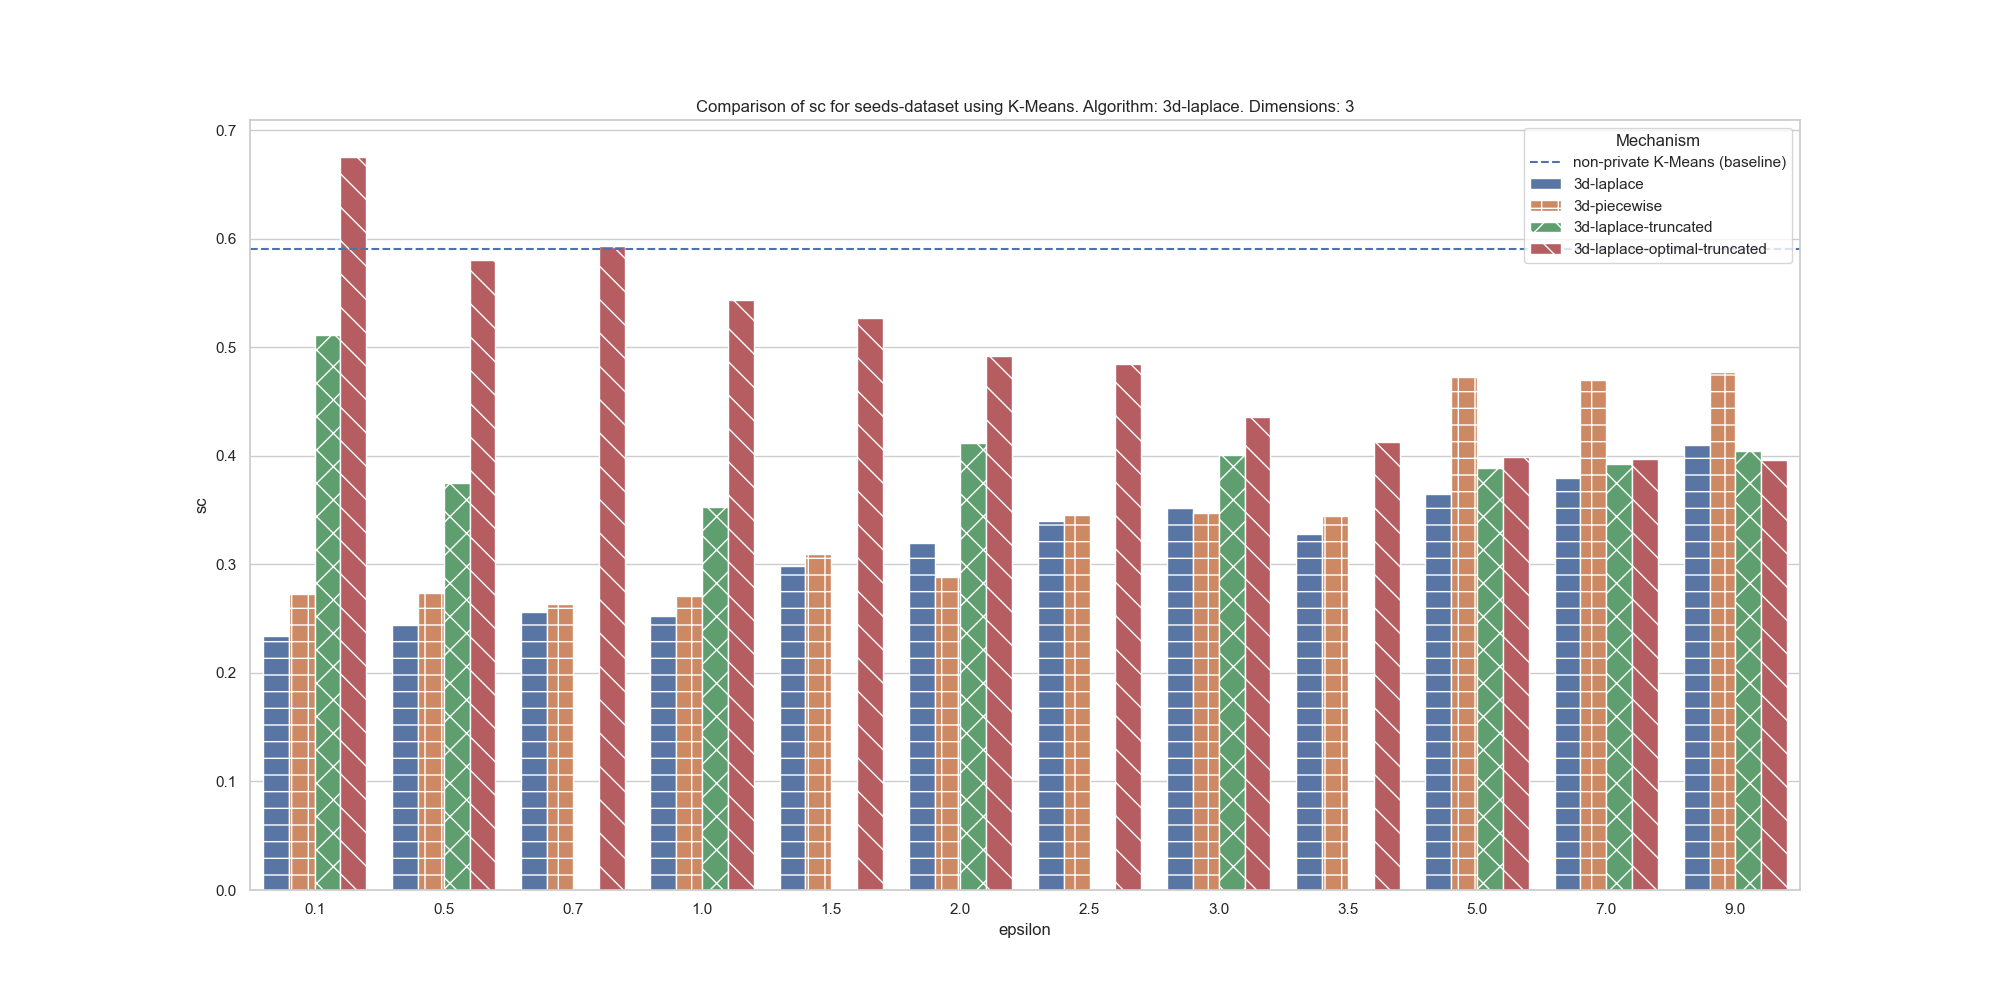
\includegraphics[width=1\textwidth]{Results/RQ2/seeds-dataset/sc_seeds-dataset_comparison.png}
        \caption{Silhouette score comparison for the 3D seeds-dataset}
        \label{fig:appendix-sc_seeds-dataset_comparison_3d}
    \end{minipage}
    \begin{minipage}[c]{0.8\textwidth}
        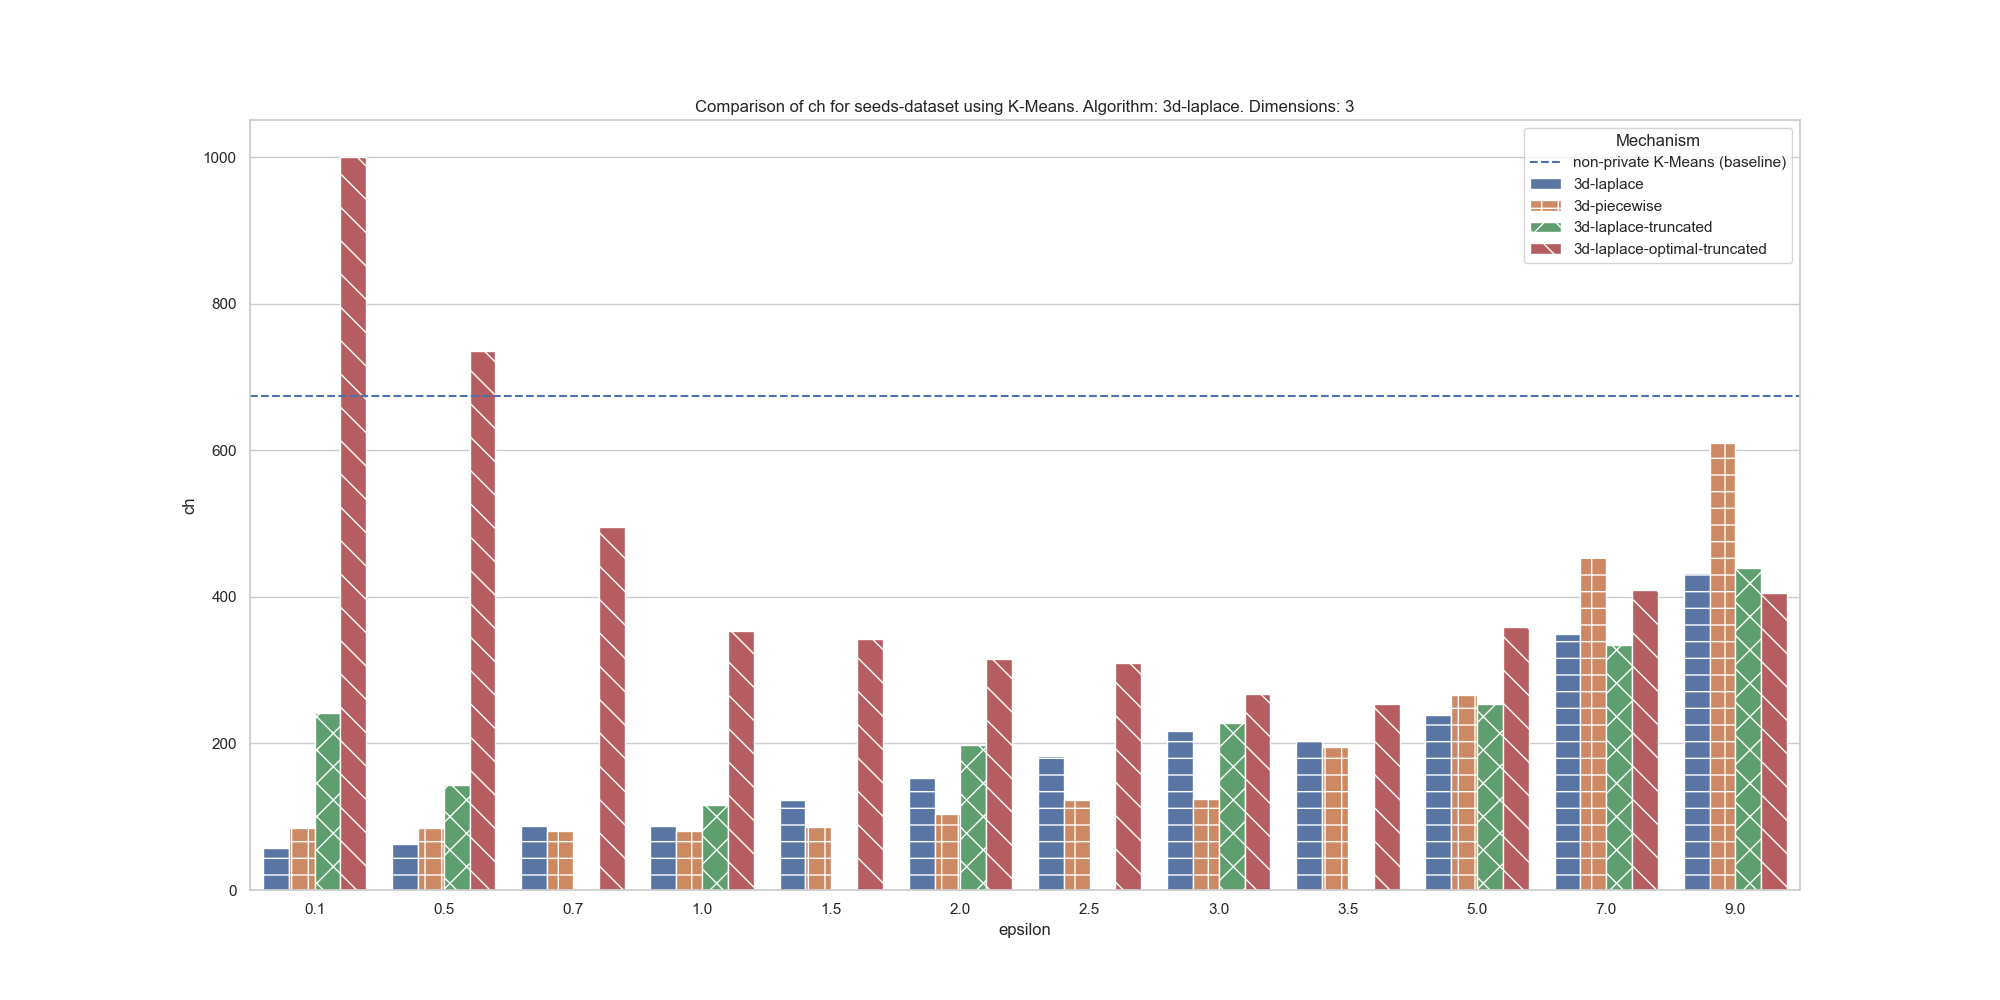
\includegraphics[width=1\textwidth]{Results/RQ2/seeds-dataset/ch_seeds-dataset_comparison.png}
        \caption{Calinski Harabasz score comparison for the 3D seeds-dataset}
        \label{fig:appendix-ch_seeds-dataset_comparison_3d}
    \end{minipage}

\end{figure}
\begin{figure}[H]
    \centering
    \begin{minipage}[c]{0.8\textwidth}
        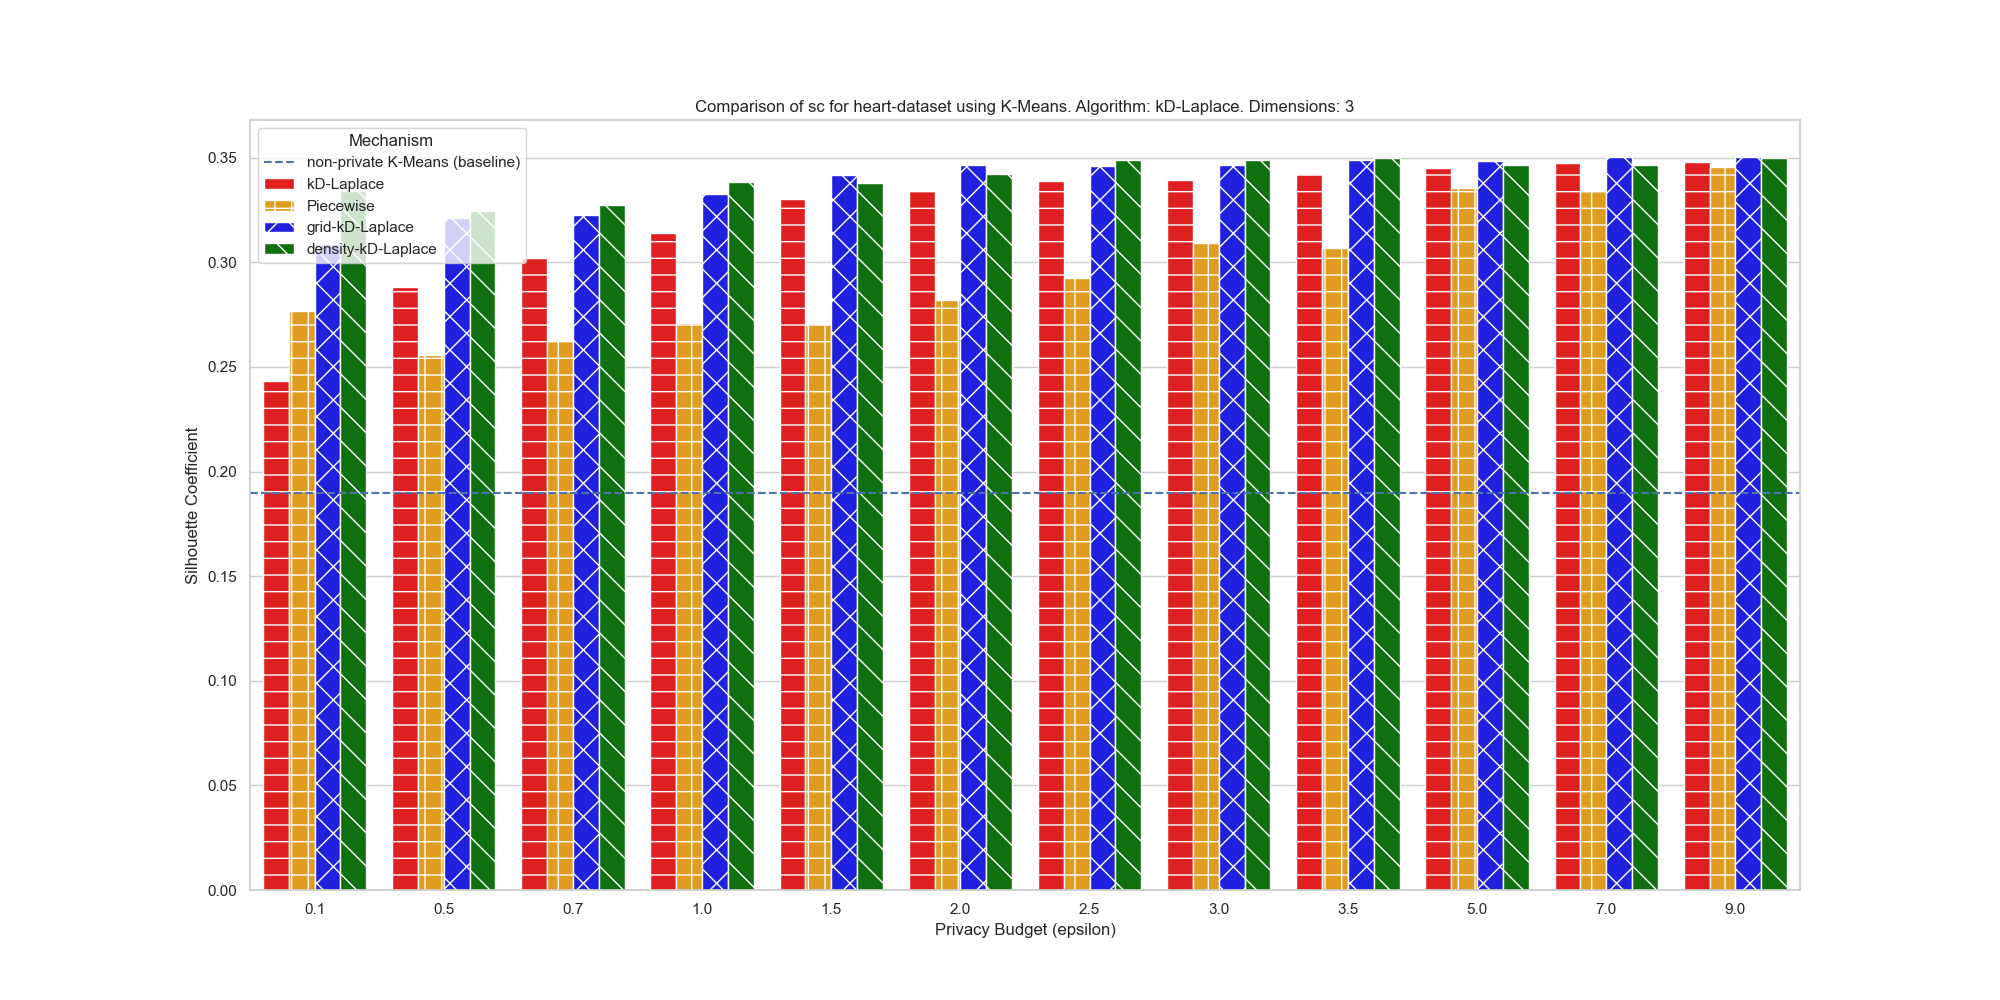
\includegraphics[width=1\textwidth]{Results/RQ2/heart-dataset/sc_heart-dataset_comparison.png}
        \caption{Silhouette score comparison for the 3D heart-dataset}
        \label{fig:appendix-sc_heart-dataset_comparison_3d}
    \end{minipage}
    \begin{minipage}[c]{0.8\textwidth}
        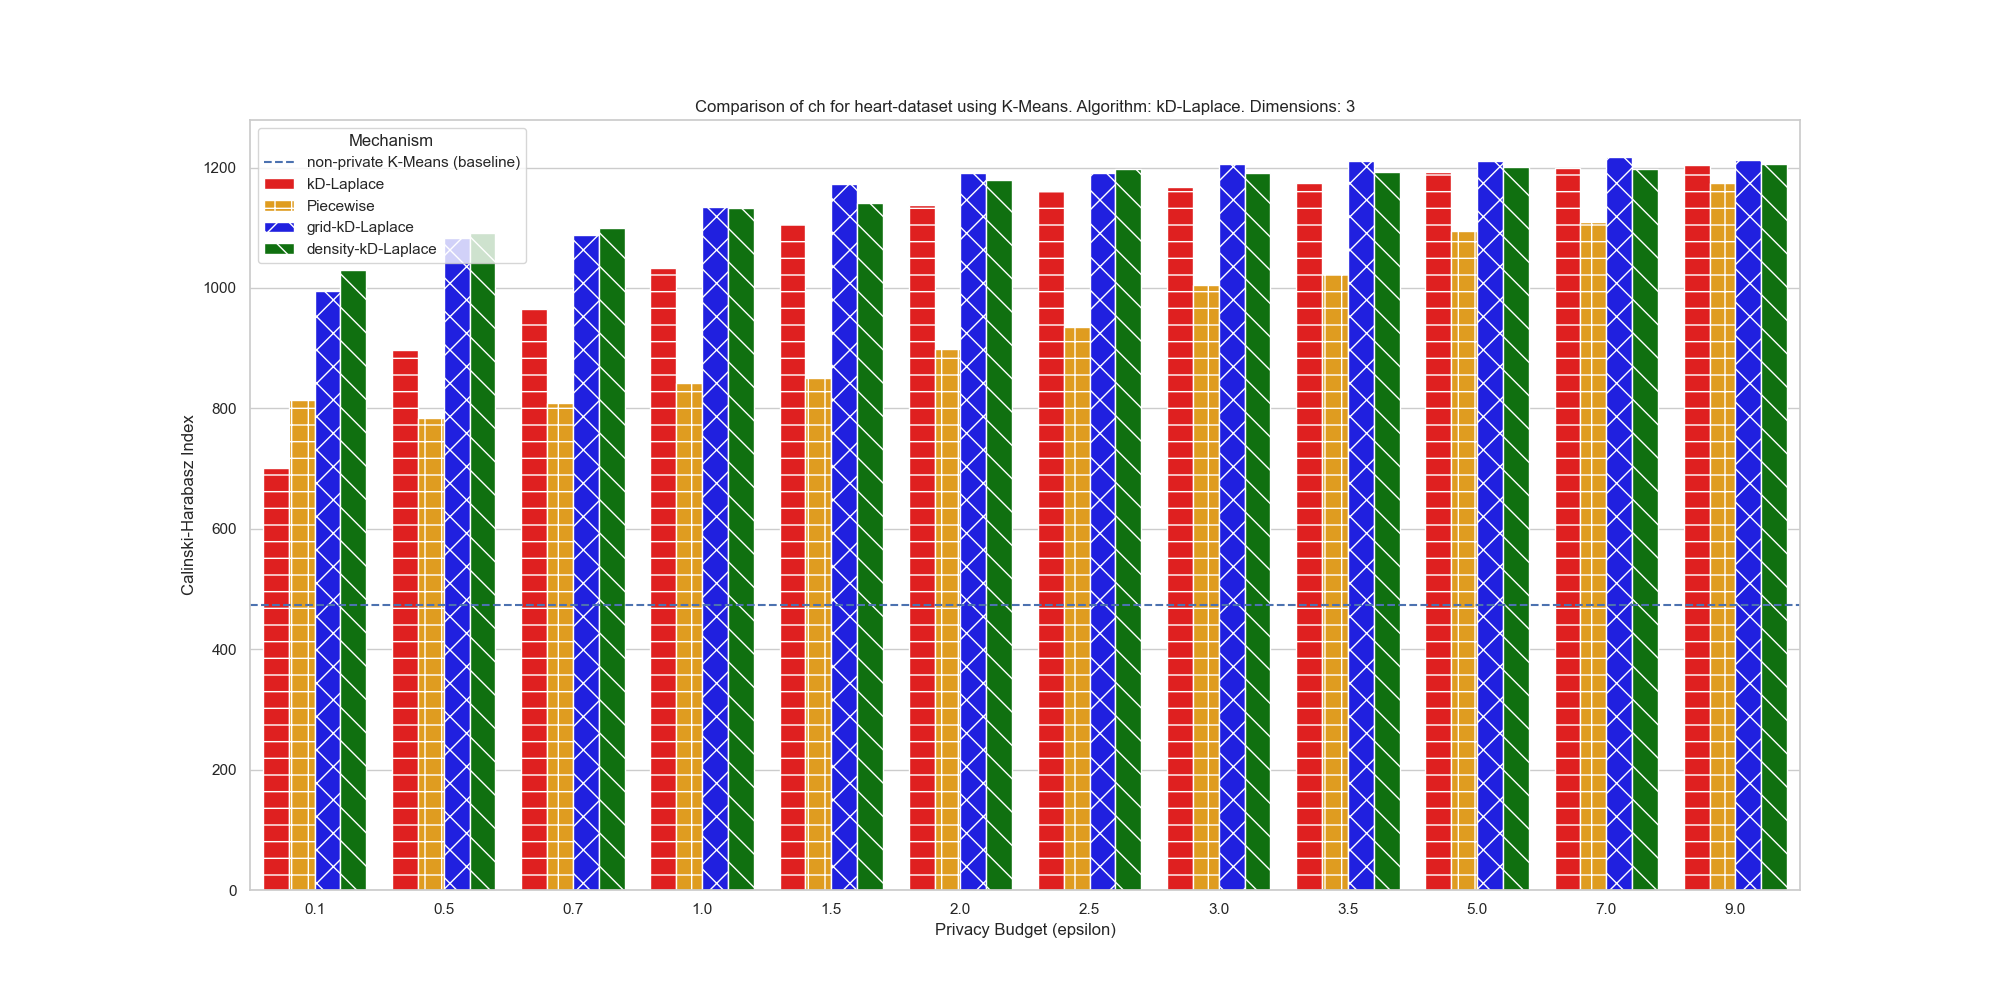
\includegraphics[width=1\textwidth]{Results/RQ2/heart-dataset/ch_heart-dataset_comparison.png}
        \caption{Calinski Harabasz score comparison for the 3D heart-dataset}
        \label{fig:appendix-ch_heart-dataset_comparison_3d}
    \end{minipage}

\end{figure}
\subsection{n-Dimensional data}
\begin{figure}[H]
    \centering
    \begin{minipage}[c]{0.8\textwidth}
        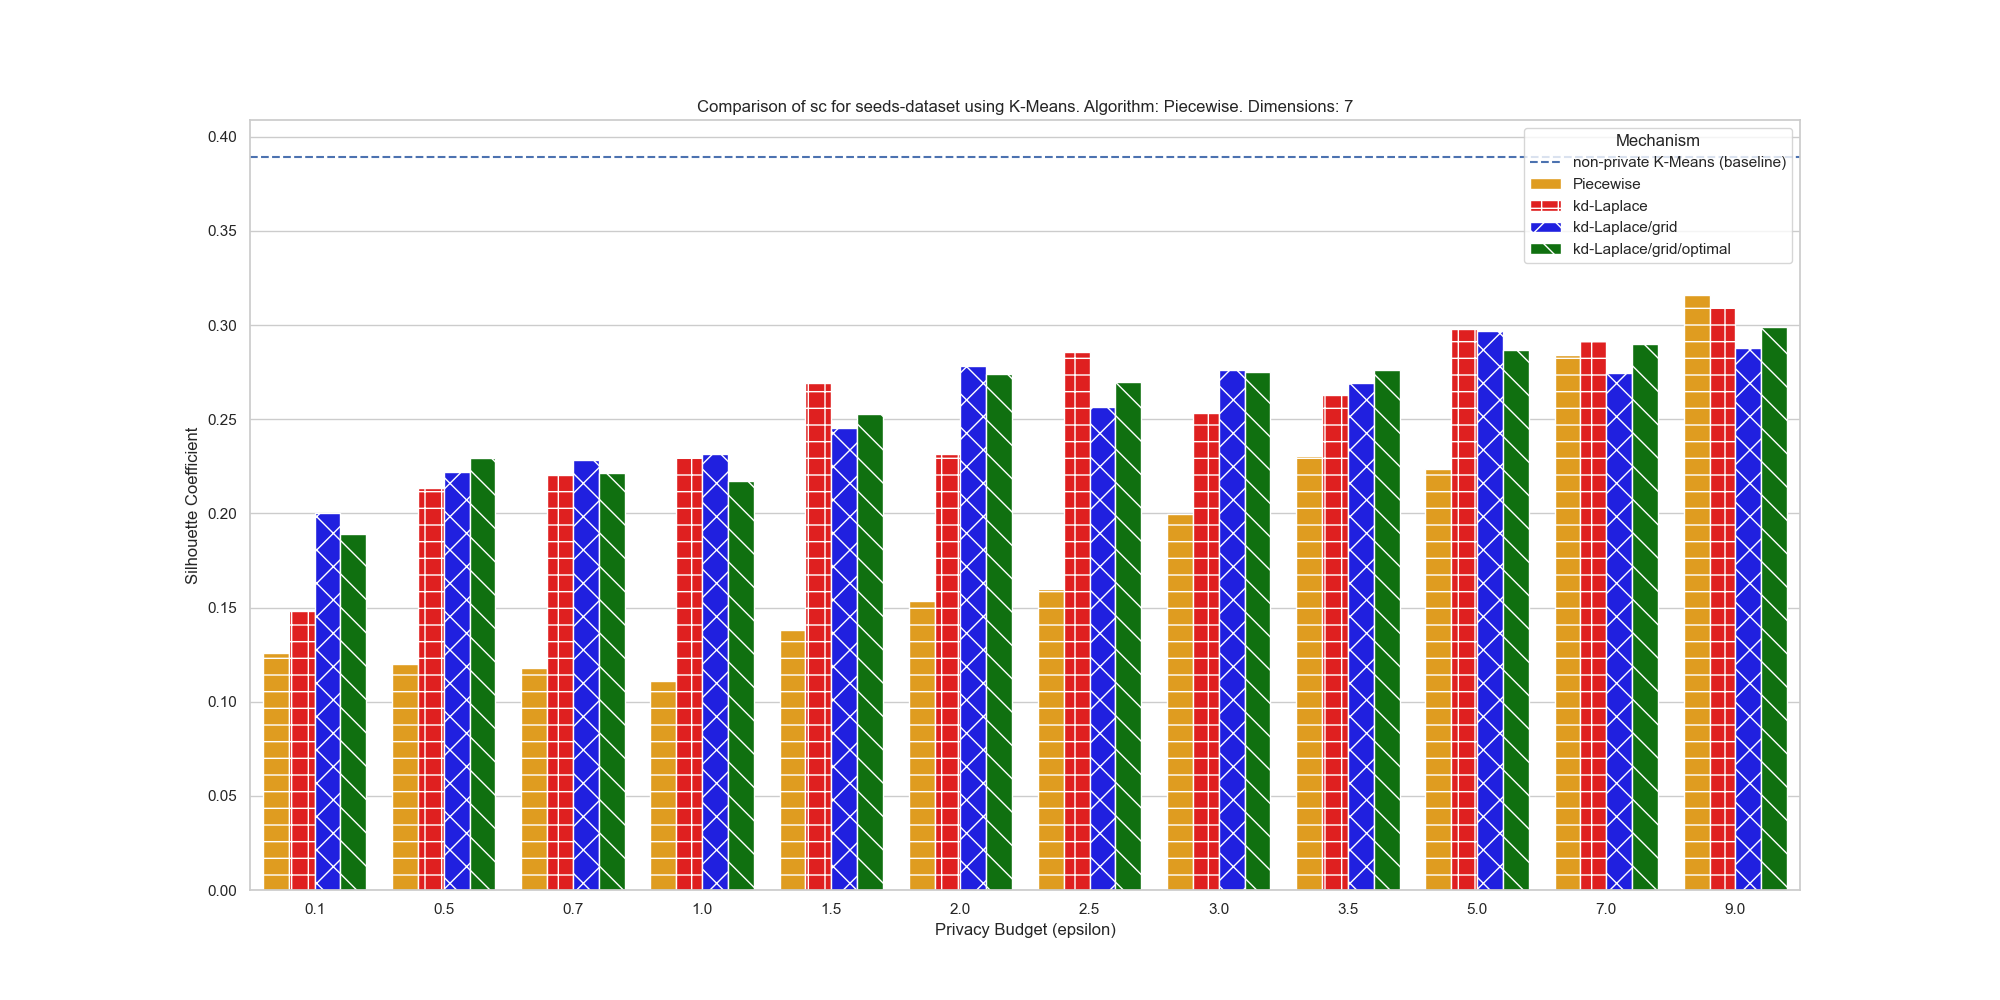
\includegraphics[width=1\textwidth]{Results/RQ2-nd/seeds-dataset/sc_seeds-dataset_comparison.png}
        \caption{Silhouette score comparison for the nd seeds-dataset}
        \label{fig:appendix-sc_seeds-dataset_comparison_nd}
    \end{minipage}
    \begin{minipage}[c]{0.8\textwidth}
        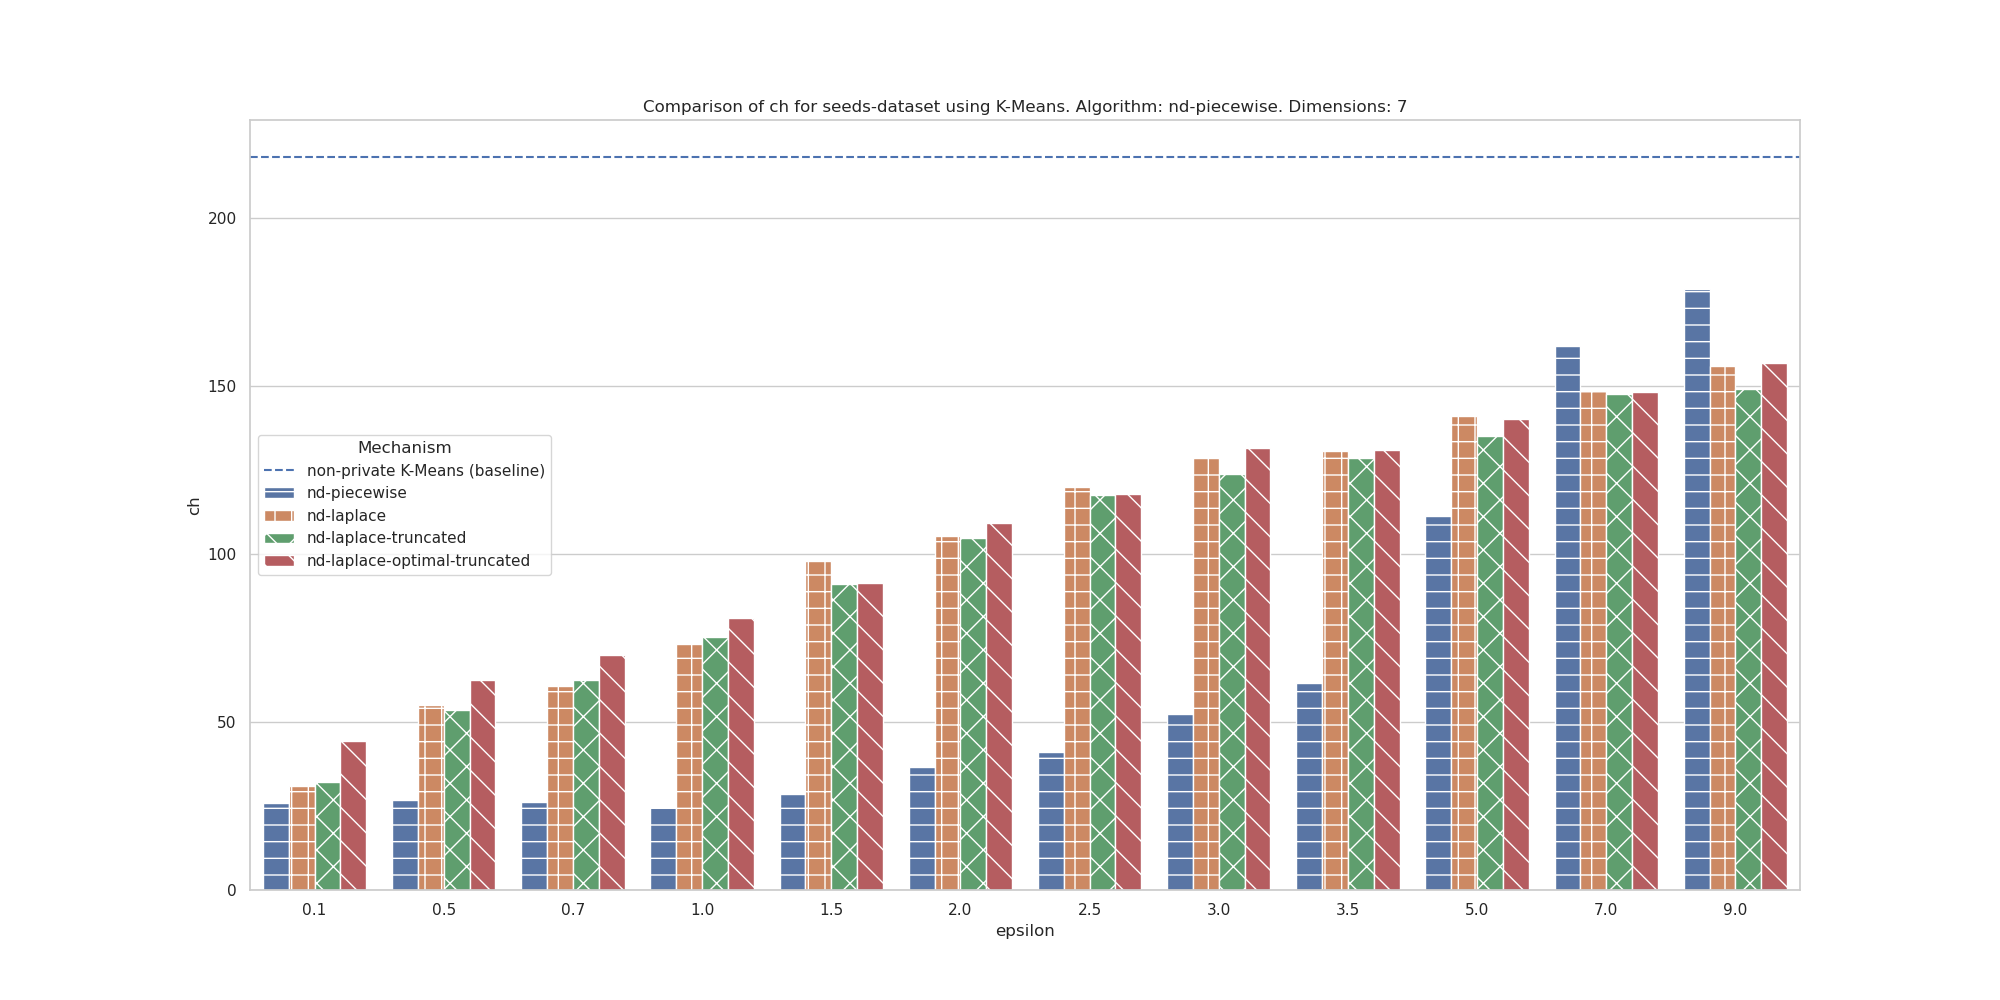
\includegraphics[width=1\textwidth]{Results/RQ2-nd/seeds-dataset/ch_seeds-dataset_comparison.png}
        \caption{Calinski Harabasz score comparison for the nd seeds-dataset}
        \label{fig:appendix-ch_seeds-dataset_comparison_nd}
    \end{minipage}
\end{figure}
\begin{figure}[H]
    \centering
    \begin{minipage}[c]{0.8\textwidth}
        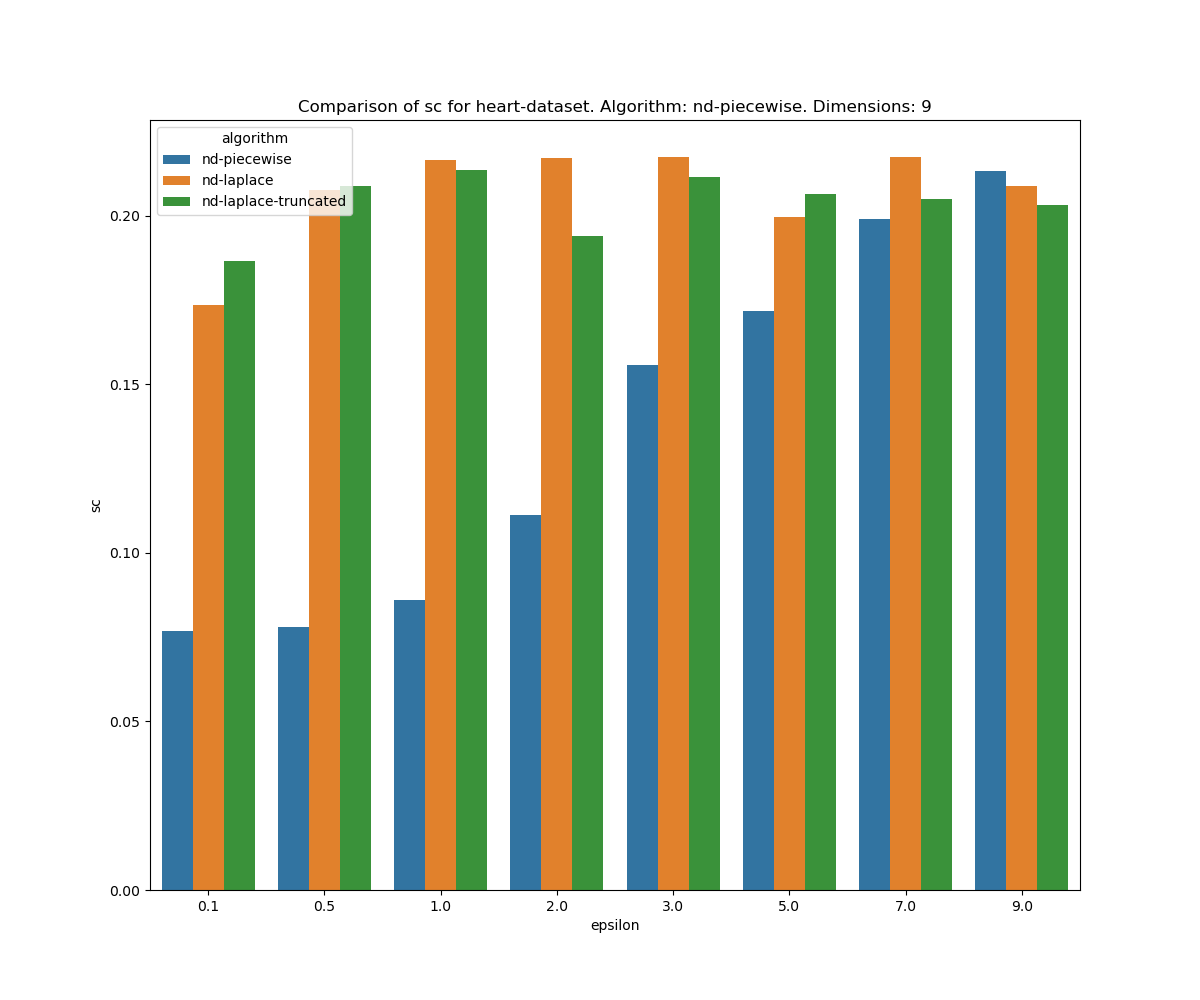
\includegraphics[width=1\textwidth]{Results/RQ2-nd/heart-dataset/sc_heart-dataset_comparison.png}
        \caption{Silhouette score comparison for the nd heart-dataset}
        \label{fig:appendix-sc_heart-dataset_comparison_nd}
    \end{minipage}
    \begin{minipage}[c]{0.8\textwidth}
        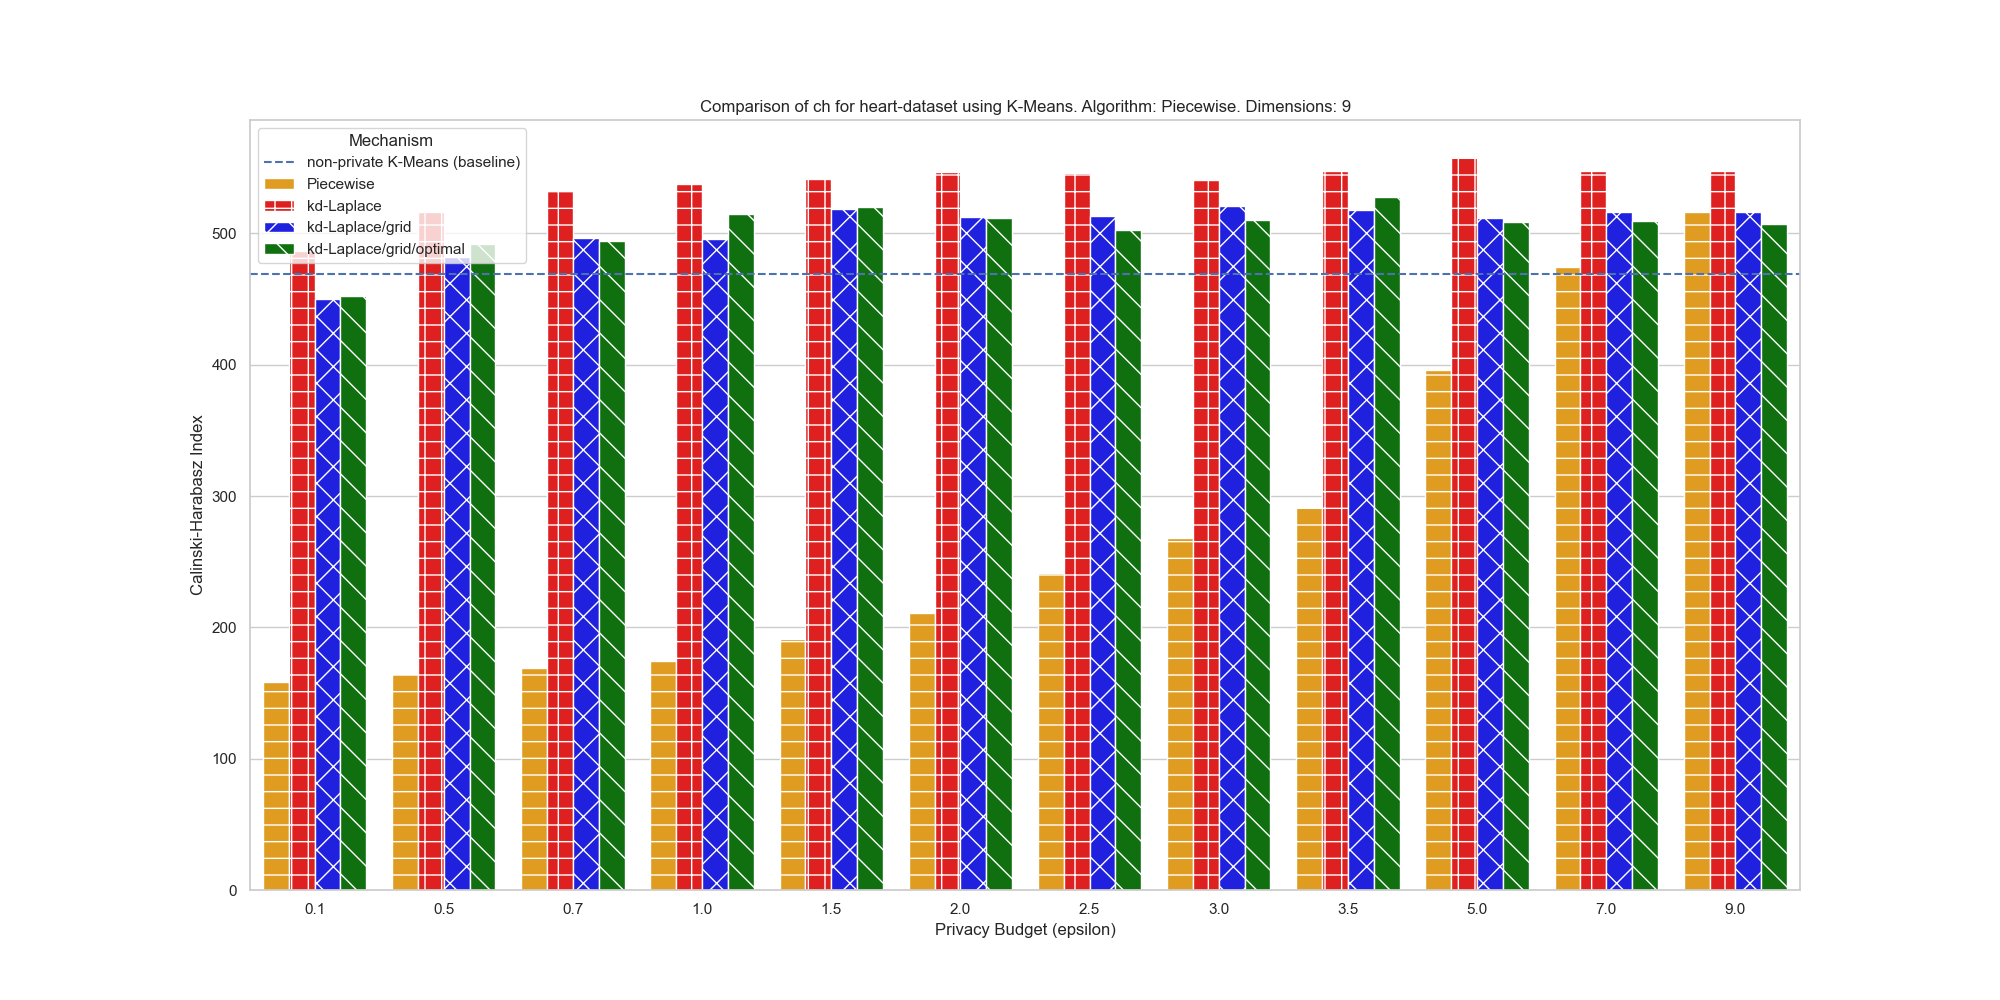
\includegraphics[width=1\textwidth]{Results/RQ2-nd/heart-dataset/ch_heart-dataset_comparison.png}
        \caption{Calinski Harabasz score comparison for the nd heart-dataset}
        \label{fig:appendix-ch_heart-dataset_comparison_nd}
    \end{minipage}

\end{figure}
\mycomment{\section{Privacy} \label{appendix:privacy}
    \subsection{2-dimensional data}
    \begin{figure}[H]
        \centering
        \begin{minipage}[c]{0.8\textwidth}
            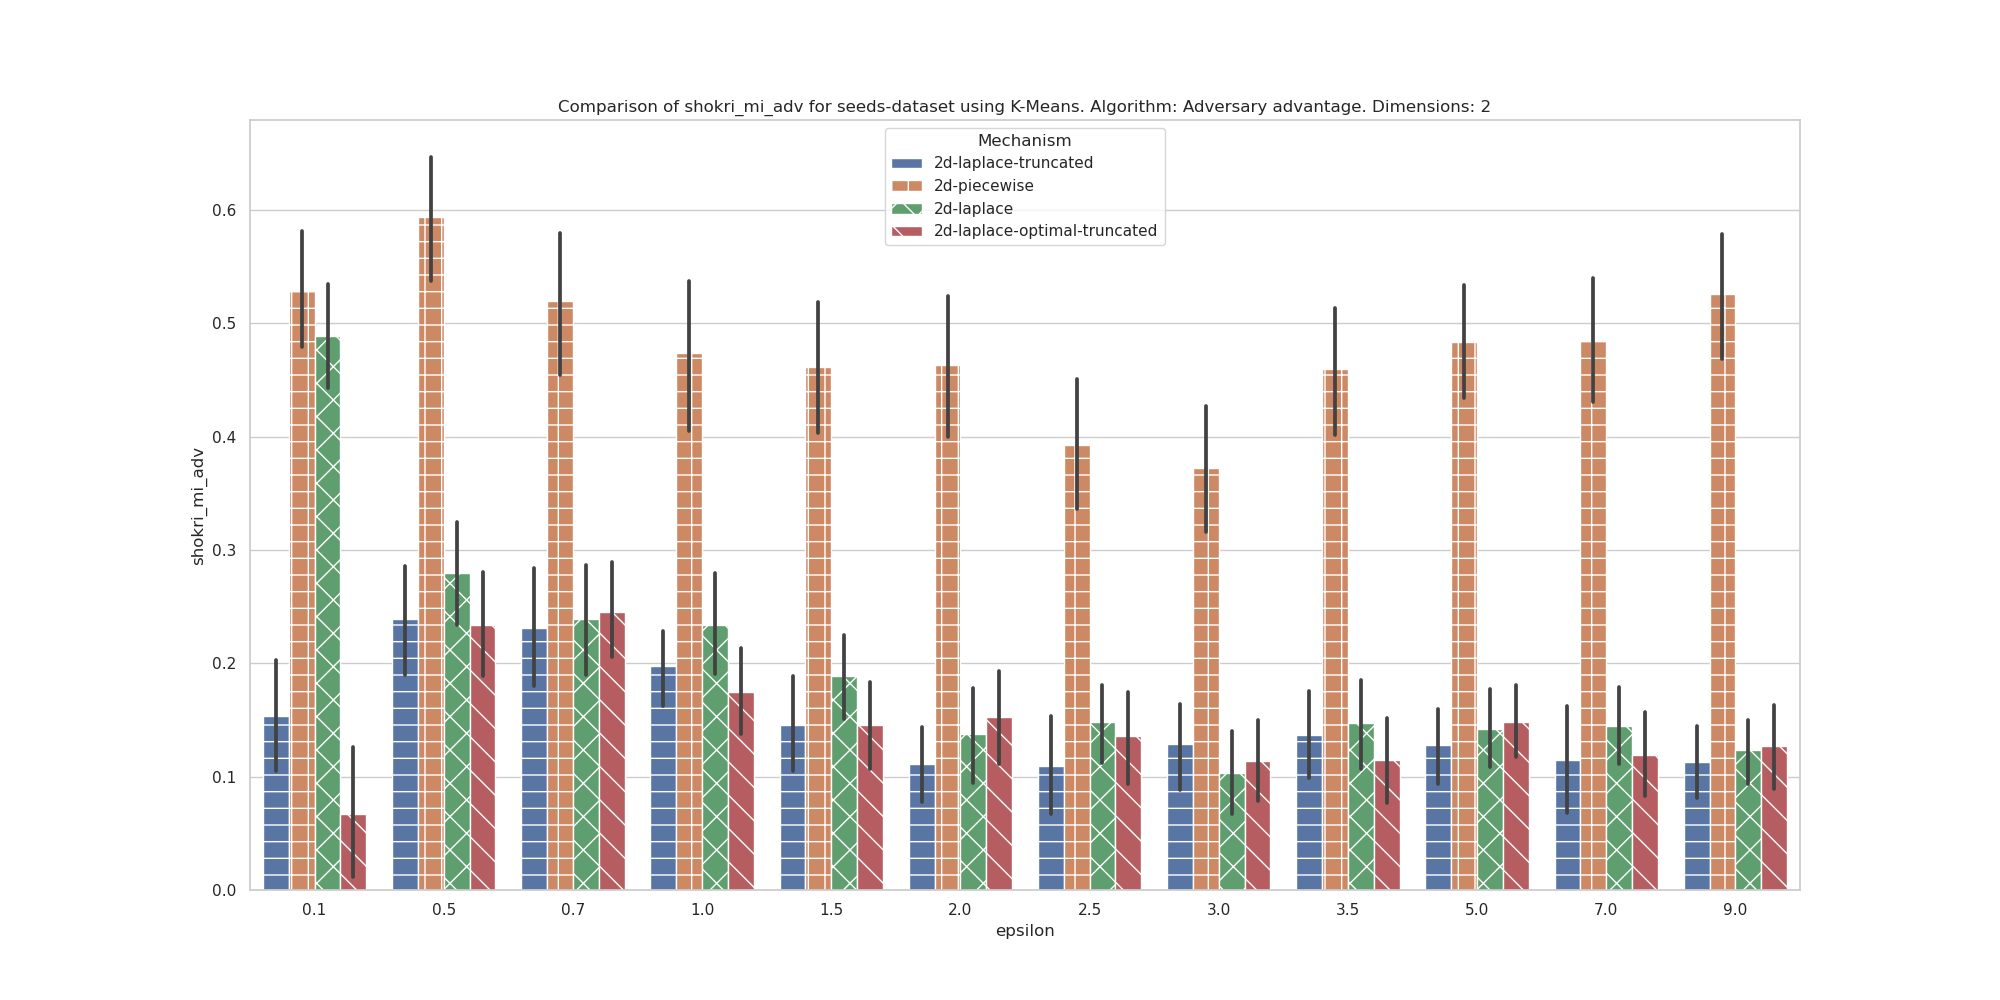
\includegraphics[width=1\textwidth]{Results/RQ1/seeds-dataset/shokri_mi_adv_seeds-dataset_comparison.png}
            \caption{Adversary advantage comparison for the 2D seeds-dataset}
            \label{fig:appendix-mi_seeds-dataset_comparison_2d}
        \end{minipage}
        \begin{minipage}[c]{0.8\textwidth}
            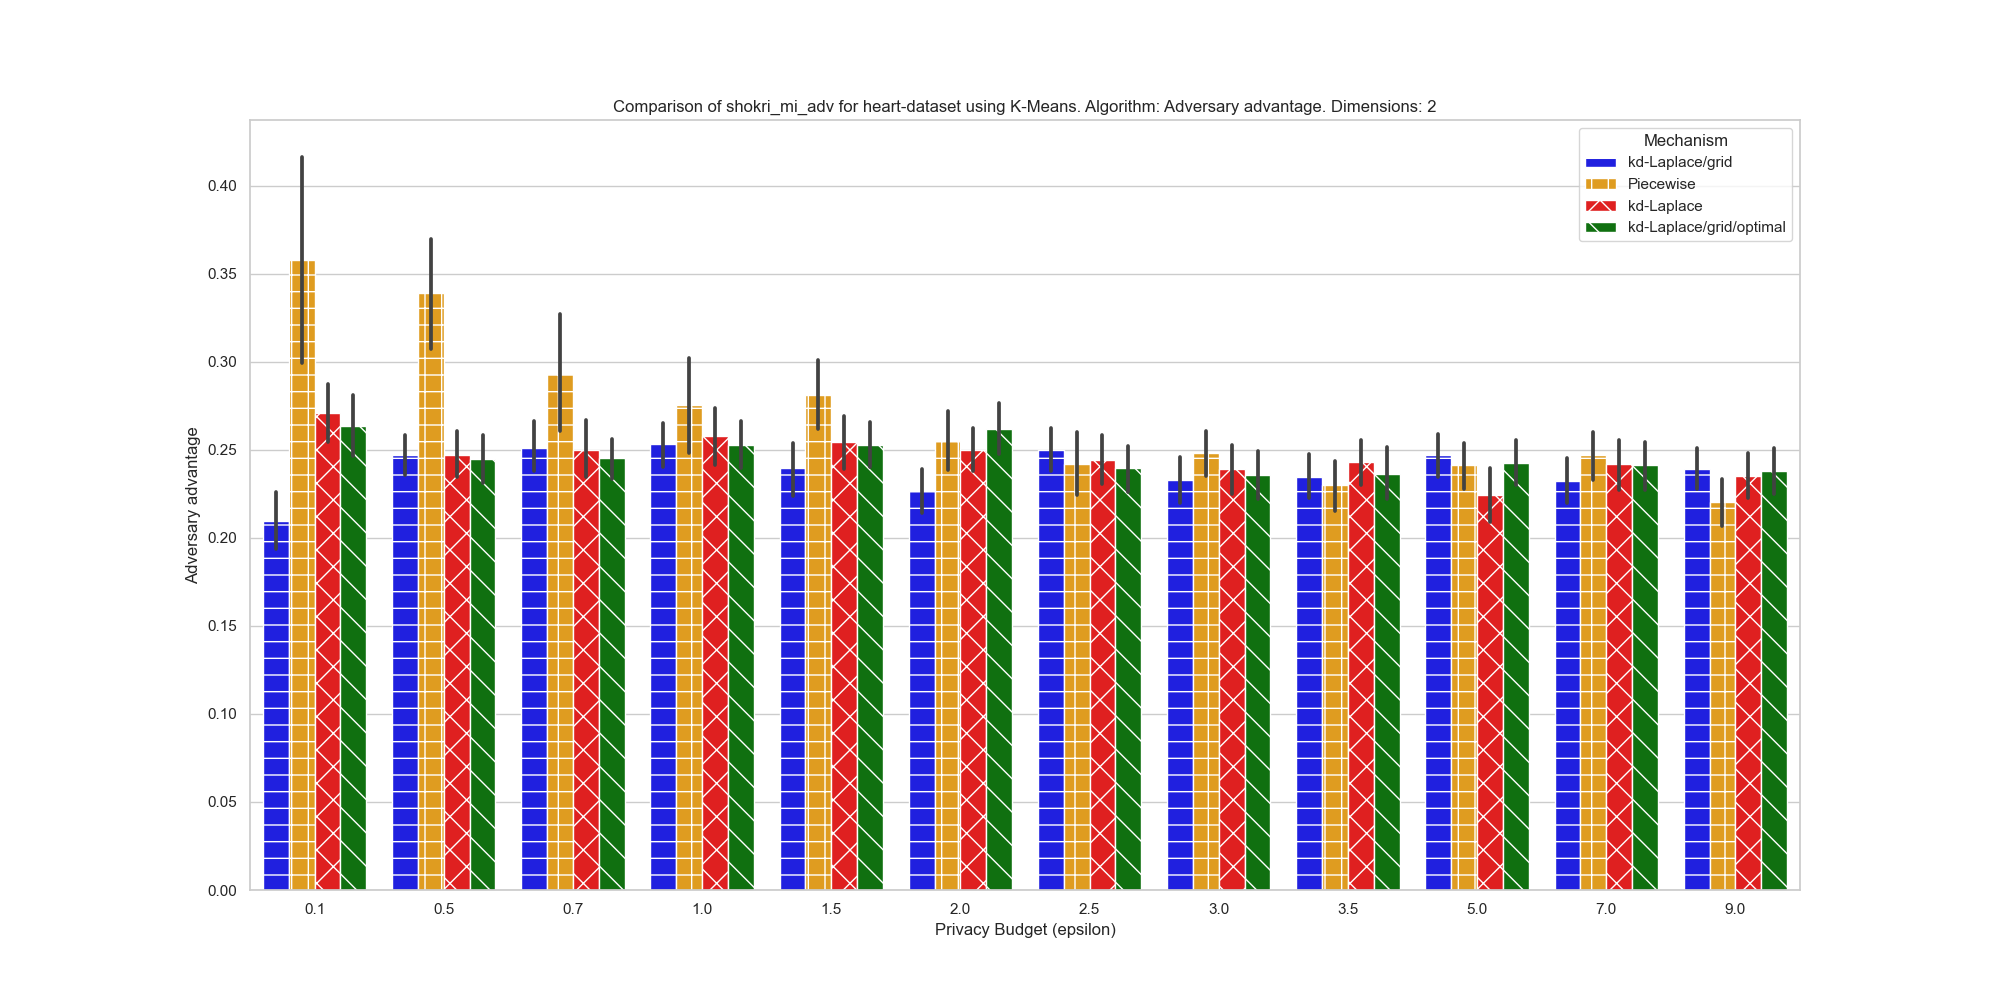
\includegraphics[width=1\textwidth]{Results/RQ1/heart-dataset/shokri_mi_adv_heart-dataset_comparison.png}
            \caption{Adversary advantage comparison for the 2D heart-dataset}
            \label{fig:appendix-mi_heart-dataset_comparison_2d}
        \end{minipage}

    \end{figure}
    \subsection{3-Dimensional data}
    \begin{figure}[H]
        \centering
        \begin{minipage}[c]{0.8\textwidth}
            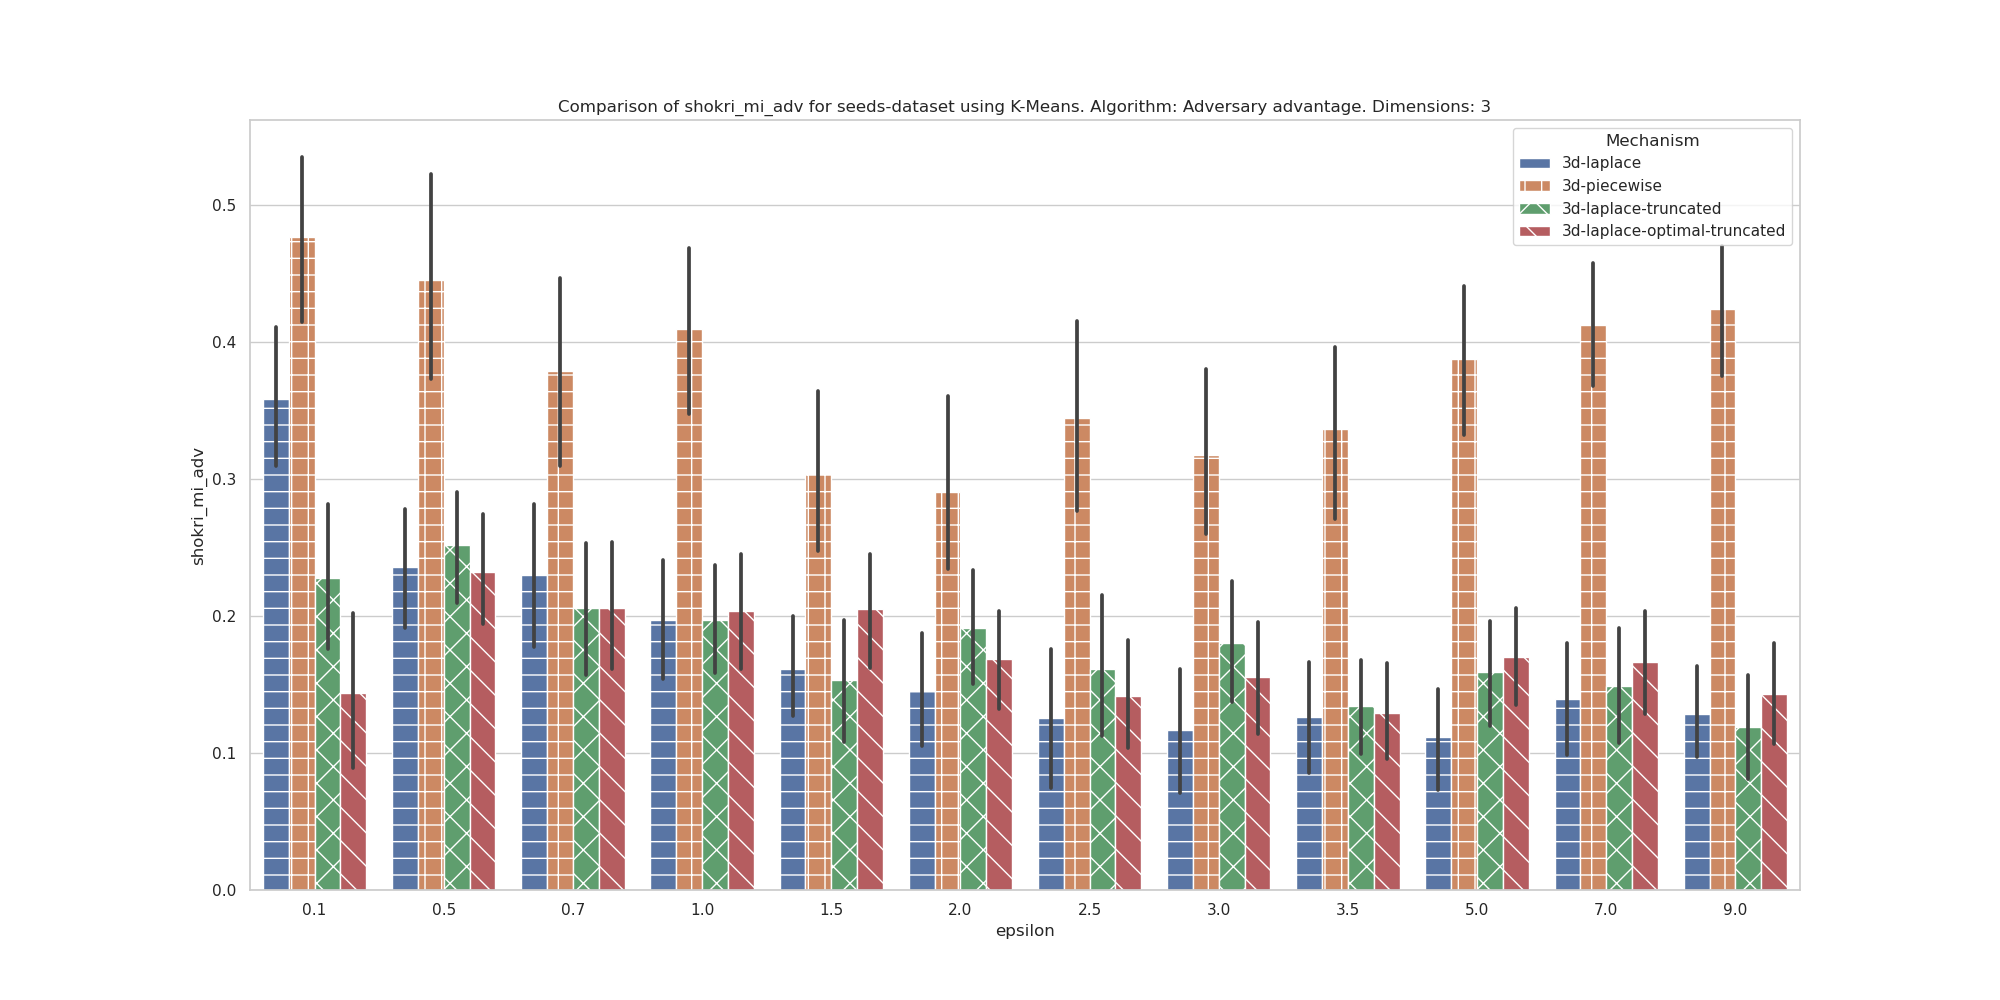
\includegraphics[width=1\textwidth]{Results/RQ2/seeds-dataset/shokri_mi_adv_seeds-dataset_comparison.png}
            \caption{Adversary advantage comparison for the 3D seeds-dataset}
            \label{fig:appendix-mi_seeds-dataset_comparison_3 d}
        \end{minipage}
        \begin{minipage}[c]{0.8\textwidth}
            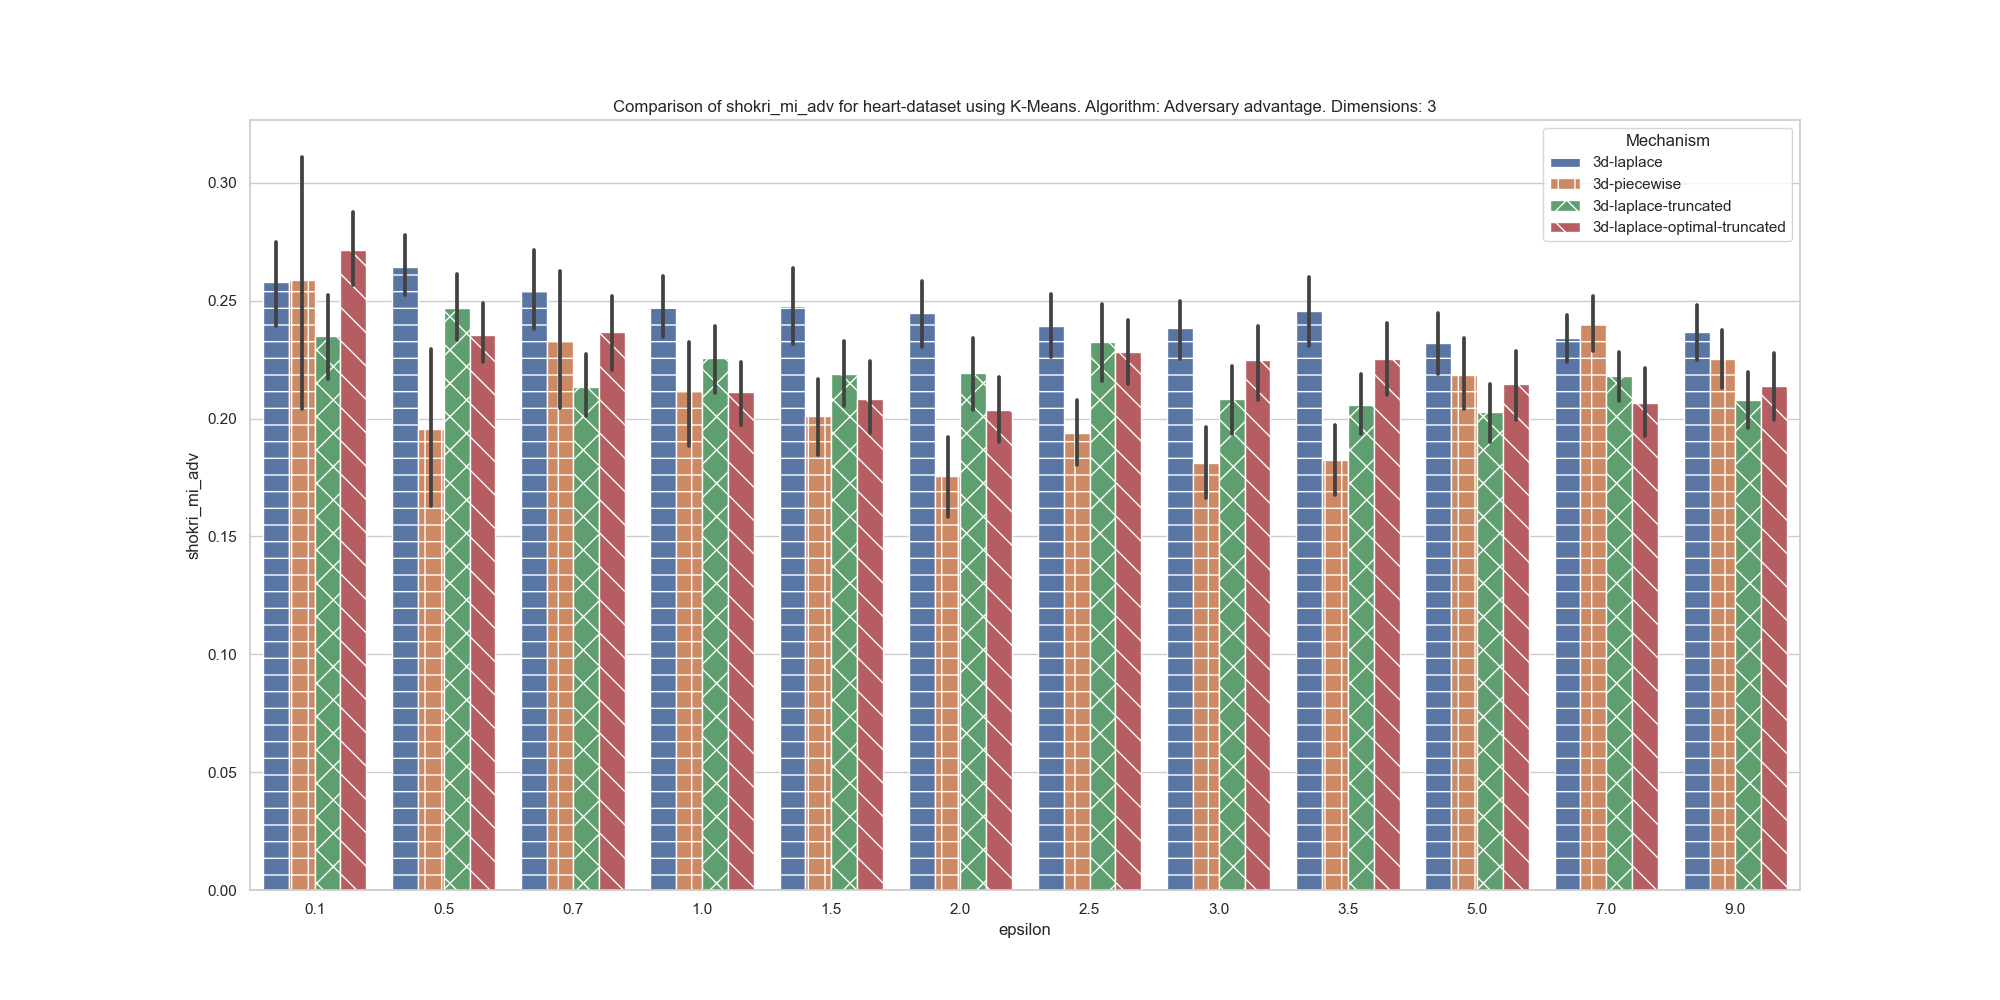
\includegraphics[width=1\textwidth]{Results/RQ2/heart-dataset/shokri_mi_adv_heart-dataset_comparison.png}
            \caption{Adversary advantage comparison for the 3D heart-dataset}
            \label{fig:appendix-mi_heart-dataset_comparison_3d}
        \end{minipage}

    \end{figure}
    \subsection{n-Dimensional data}
    \begin{figure}[H]
        \centering
        \begin{minipage}[c]{0.8\textwidth}
            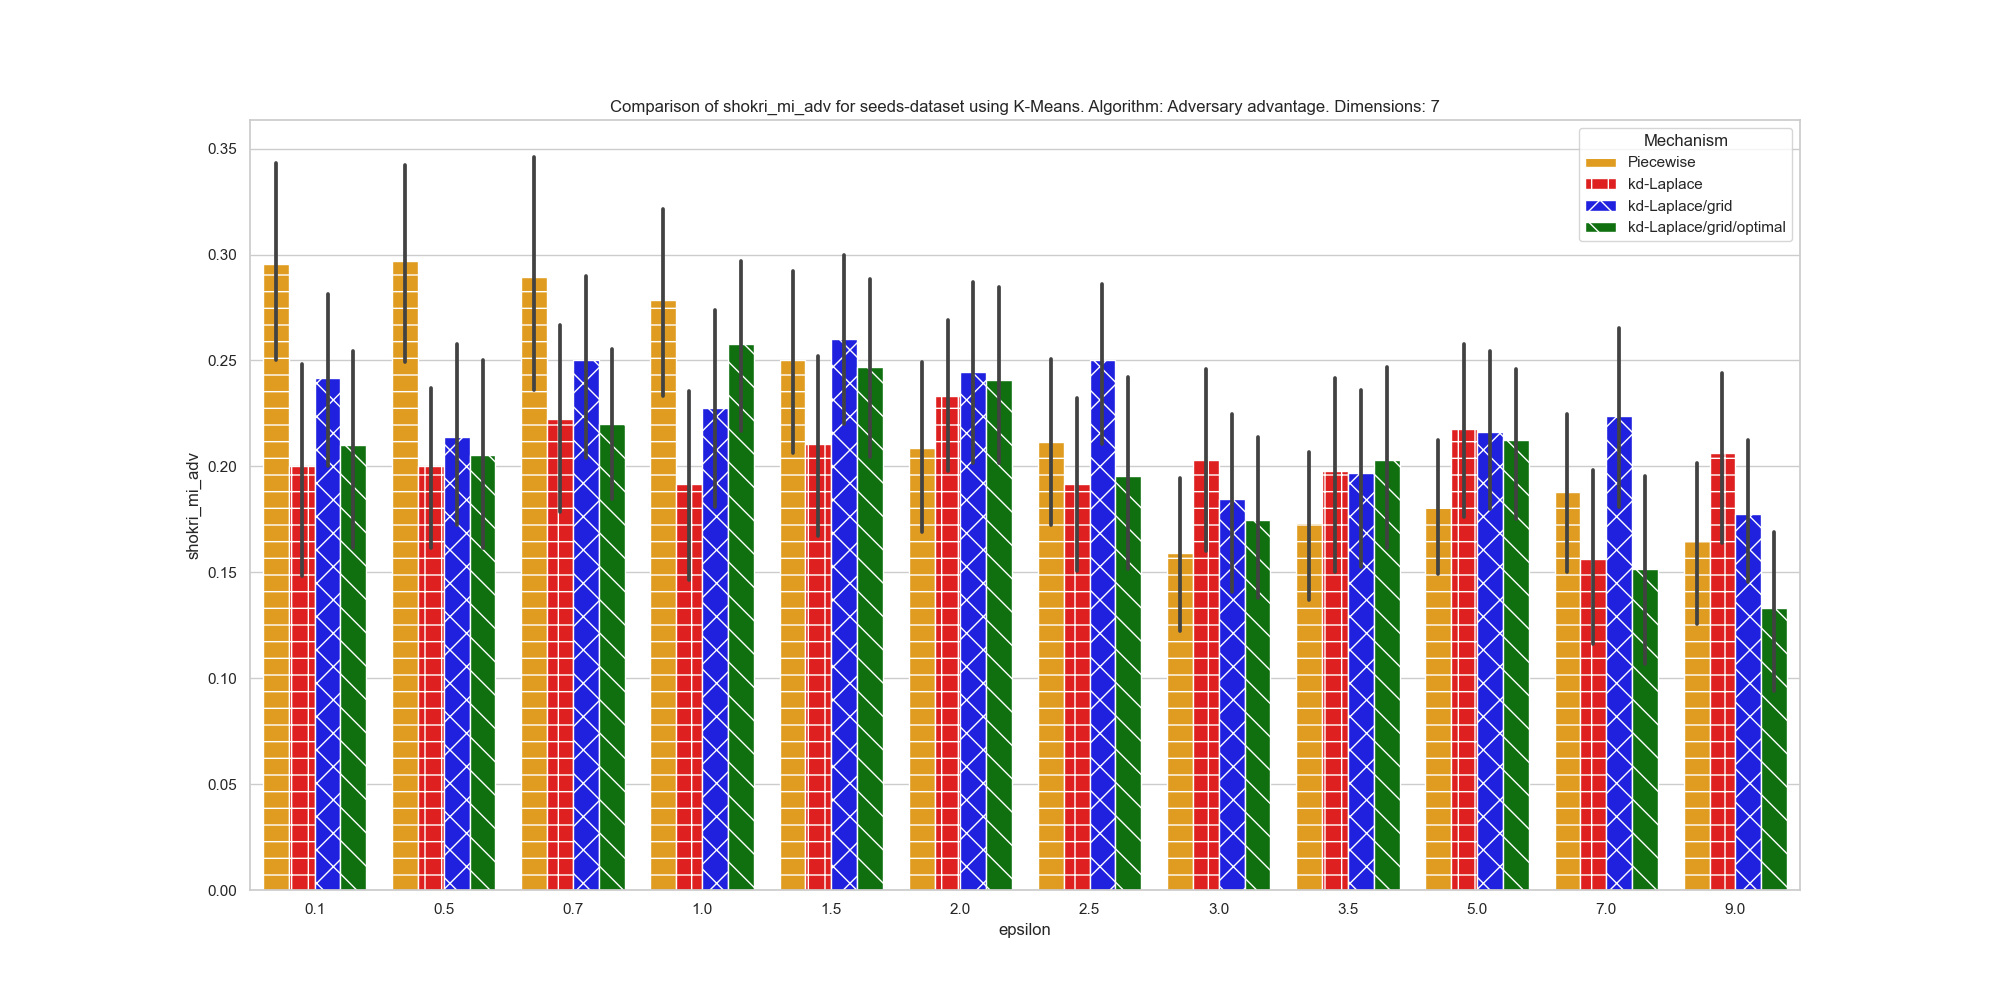
\includegraphics[width=1\textwidth]{Results/RQ2-nd/seeds-dataset/shokri_mi_adv_seeds-dataset_comparison.png}
            \caption{Adversary advantage comparison for the nD seeds-dataset}
            \label{fig:appendix-mi_seeds-dataset_comparison_nd}
        \end{minipage}
        \begin{minipage}[c]{0.8\textwidth}
            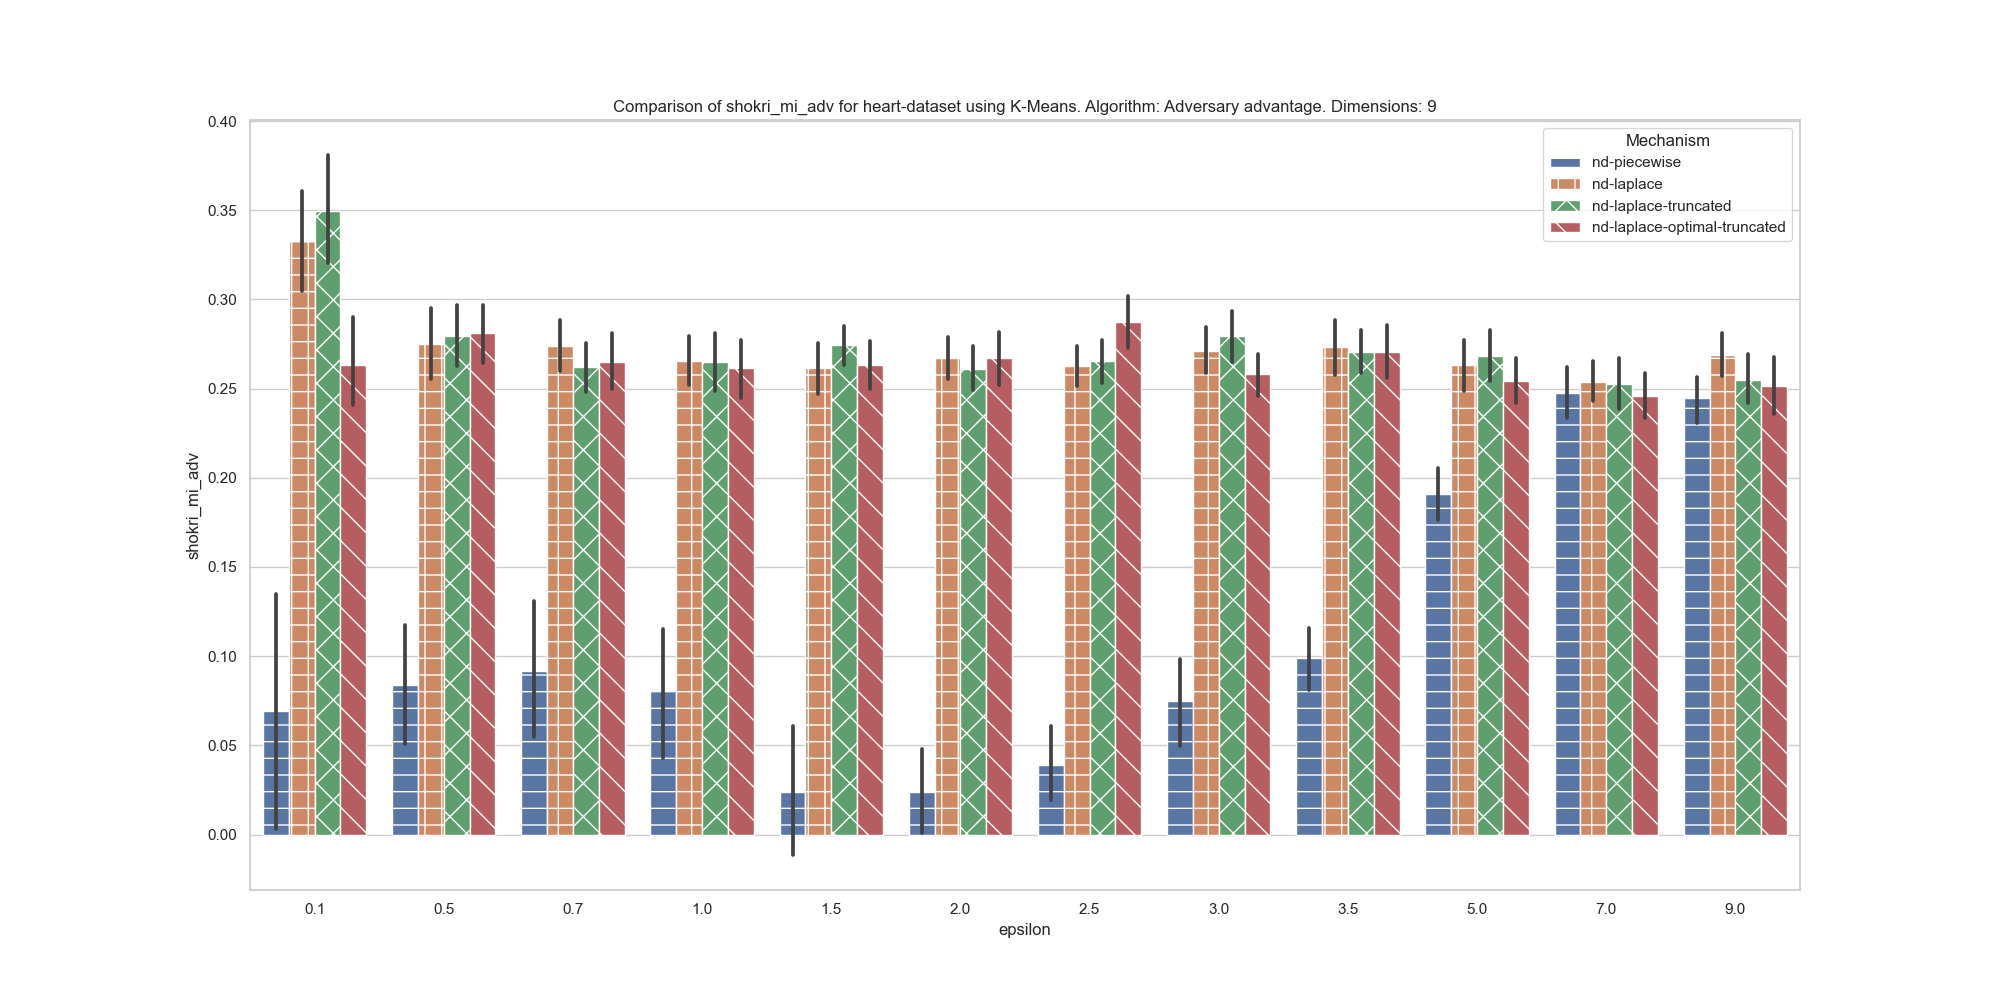
\includegraphics[width=1\textwidth]{Results/RQ2-nd/heart-dataset/shokri_mi_adv_heart-dataset_comparison.png}
            \caption{Adversary advantage comparison for the nD heart-dataset}
            \label{fig:appendix-mi_heart-dataset_comparison_nd}
        \end{minipage}

    \end{figure}}
%\section{Dimensionality}